\documentclass{article}
\usepackage[utf8]{inputenc}
\usepackage{amsmath}
\usepackage{natbib}
\usepackage{parskip}
\usepackage{tikz}
\bibliographystyle{jasa}
\usetikzlibrary{positioning,calc,backgrounds}
\usepackage{thmtools}
\usepackage{lipsum}
%\usepackage{blindtext}
\usepackage{xcolor}
\usepackage{comment}



\title{Notater til masteren}
\author{johaskog }
\date{January 2021}

\parskip 0.2in %making spacing between paragraphs
\newcommand{\dd}{\mathrm{d}}
%\newtheorem{theorem}{Theorem}
\colorlet{myblue}{blue!5!white}
%\definecolor{myblue}{rgb}{188,217,255}
%\definecolor{myblue}{rgb}{1,1,1}

\declaretheorem[
  shaded={rulecolor=black, rulewidth=1pt, bgcolor=myblue},
  name=Theorem,
]{theorem}





\begin{document}

\maketitle
%need this to plot the tikz trees. 
%This is needed for the tikzpicture:
\newcommand{\DoNode}[8][]{% (keys), name, loss1, loss2, loss3, CircleColour1, CircleColour2, radius
    %\pgfmathtruncatemacro{\tmpa}{round(360*#3/(#3+#4+#5))}
    %\pgfmathtruncatemacro{\tmpb}{round(360*(#3+#4)/(#3+#4+#5))}
    %\pgfmathtruncatemacro{\tmpa}{round(360*(#3/(#3+#4+#5)))}
    %\pgfmathtruncatemacro{\tmpb}{round(360*((#3+#4)/(#3+#4+#5)))}
    \pgfmathtruncatemacro{\tmpa}{round(360*(#3/(#3+#4+#5)))+90}
    \pgfmathtruncatemacro{\tmpb}{round(360*((#3+#4)/(#3+#4+#5)))+90}
    
    %\node[treenodeT, #1] (#2) {Loss0: #3 \\ Loss1: #4 \\ Loss2: #5};
    \node[treenodeT, #1, minimum size=2*#8cm] (#2) {};
    % and after that...
    \begin{scope}[on background layer]
        %\fill [blue!40] let \p1 = ($(#2.0)-(#2.center)$) in
        %    (#2.center) -- (#2.0) arc(0:\tmpa:{veclen(\x1,\y1)}) -- cycle;
        %\fill [red!40] let \p1 = ($(#2.0)-(#2.center)$) in
        %    (#2.center) -- (#2.\tmpa) arc(\tmpa:\tmpb:{veclen(\x1,\y1)}) -- cycle;
        %\fill [green!30] let \p1 = ($(#2.0)-(#2.center)$) in
        %    (#2.center) -- (#2.\tmpb) arc(\tmpb:360:{veclen(\x1,\y1)}) -- cycle;
        \fill [blue!30] let \p1 = ($(#2.0)-(#2.center)$) in
            (#2.center) -- (#2.0) arc(0:\tmpa:{veclen(\x1,\y1)}) -- cycle;
        \fill [red!30] let \p1 = ($(#2.0)-(#2.center)$) in
            (#2.center) -- (#2.\tmpa) arc(\tmpa:\tmpb:{veclen(\x1,\y1)}) -- cycle;
        \fill [green!30] let \p1 = ($(#2.0)-(#2.center)$) in
            (#2.center) -- (#2.\tmpb) arc(\tmpb:450:{veclen(\x1,\y1)}) -- cycle;
%        \draw [#6!20] let \p1 = ($(#2.0)-(#2.center)$) in
%            (#2.center) -- (#2.\tmpb) arc(\tmpb:360:{veclen(\x1,\y1)}) -- cycle;
%        \draw[color = #6] (#2.center) circle (1.5cm);
        \draw[color= #6, very thick] (#2.center)+(0,#8cm) arc (90:270:#8cm);
        \draw[color = #7, very thick] (#2.center)+(0,-#8cm) arc (270:360:#8cm);
        \draw[color = #7, very thick] (#2.center)+(#8cm,0) arc (0:90:#8cm);
    
    \end{scope}
}


\newpage
%\section{Introduction}
\chapter{Introduction}
Schizophrenia is a psychotic disorder where at least two of the symptoms delusions, hallucinations, disorganized speech, grossly disorganized or catatonic behaviour or negative symptoms such as reduced emotional expressions and lowered motivation, have to be present. 
Delusions are beliefs that will not change if contradicting evidence is presented. The most common type of delusions are persecutory delusions. People that have those kinds of delusions might think that they will be hurt, injured, tormented or so on by others. Referential delusions are also common. Then one are putting meaning into comments, gestures and actions, thinking that they are about oneself, when they not necessarily are. Completely improbable beliefs are called bizarre delusions. These are delusions others find far-fetched, and they are things that cannot happen in real life. A bizarre delusion could for example be that a person believes that their organs have been removed replaced by someone else's organs without there being any scars or other evidence of that happening. A delusion that is not bizarre could be that you think you are under police surveillance without there being any evidence of that. It might be hard to distinguish between delusions and strongly held ideas. The main distinction is about the degree of conviction, and how much or little the beliefs can be amended when contradicting facts are presented \citep{dsm-5}. 
%Hallucinations are sensory impressions that happen without any external stimulus. Hence, others usually does not experience the same impressions. The hallucinations are perceived as normal experiences to the person having them. For schizophrenic people, they often occur as voices which can be distinguished from the persons own thoughts. 
%Disorganized speech means that one are switching between topics rapidly and giving unrelated answers to questions. 
%Grossly disorganized behavior is also referred to as abnormal behavior, and catatonic behavior means that one has a dampened reaction to things happening around oneself. (All of the above is from DSM-5).


Delusions are one of the main characteristics of schizophrenia as it appears in about three out of four of those diagnosed \citep{garety2011}. Researchers have been trying to understand how the delusions are formed and maintained in order to improve treatment \citep{dudley_meta_2016}. One important finding is that deluded individuals seem to make decisions based on less evidence than both healthy and psychiatric controls. This is often referred to as a "jumping to conclusions" (JTC) bias \citep{dudley_meta_2016}. A person with this bias might reach decisions or form beliefs before reaching realistic conclusions, and thus accept unrealistic ideas. They are therefore more prone to delusions \citep{dudley_meta_2016}. The hope is that if we can detect the JTC bias, we can reduce the delusional thinking, and thus prevent delusions \citep{dudley_meta_2016}.

The JTC bias is traditionally tested with a probabilistic reasoning task called the beads task. The participants are presented with two jars containing beads of two colours, for example red and blue. The two jars have opposite ratios of each colour, meaning that if the first have 85\% red beads and 15\% blue, the second has 15\% red and 85\% blue beads. The participants are told that beads are drawn from one of the jars, and their task is to find out which one that is. They are told to choose only when they are completely sure, and they draw as many beads as they want. The beads are drawn sequentially, and after each draw the participants are asked if they want to choose which jar beads are drawn from or if they want to draw more beads. One are usually said to have a JTC bias if one decides after one or two beads \citep{moritz2017}. However, the beads task has shown to pose some problems.

Some of the first to use the beads task were \citet{huq1988}. Already in that article they presented some of the problems with the beads task. They used an 85-15 ratio of the beads. When the two first beads that are drawn are of the same colour, it is a 97\% probability that the beads are from the jar with 85\% of the beads in that colour. One might therefore argue that choosing jar at that point is reasonable, and that it does not show a JTC bias. Deluded individuals make decisions earlier that the control groups, but \citeauthor{huq1988} argue that non-deluded individuals are more conservative, and that people with delusions simply cancel out that bias when gathering less information. In an article by \citet{moritz2017}, other problems with the beads task are discussed. For example that many participants seem not to understand that all the beads are drawn form the same jar. This makes them think that after each bead is drawn, they have to guess which jar that bead is drawn from. These participants are then classified to have a JTC bias. We can also see that it is common to make logical errors due to miscomprehension. In an article by \citet{moritz2005}, they found that 52\% of the schizophrenic participants and 23\% of the healthy controls had at least one response that was not logical. The participants that misunderstand are more likely to choose early. \citet{moritz2017} further states that the beads task is correlated with intelligence. Lack of intelligence might be a reason for or a confound for misunderstanding the task. It is also stated that confidence influences decision-making. The participants are asked to choose when they are completely sure which jar the beads are drawn from, which could make more confident participants decide earlier. We might also conclude that hasty decisions are made because the participants like to take risks or that they are not cautious, or both. However, other tasks that accounts for confidence also display a JTC bias with the delusion-prone participants. Additionally, there is only a one-dimensional sequence of events in the beads task. Thus, it is harder to find different versions to test multiple times. 

The box task has been suggested as an alternative to the beads task. Here, the participants are presented with a grid of a fixed number of boxes. When a box is opened, one out of two colours is displayed, for example blue and red. The participants are told that one of the colours are always in majority, and their task is to find out which one \citep{moritz2017}. They can open as many boxes as they want before they make a decisions. Both the number of boxes and the ratio of the two colours can be changed for each new trial. 

In this report we model how the participants make decisions in the box task. In the version of the box task used here, there are twelve boxes. We use two different versions of the box task. The first one is an unlimited one, where the participants can open as many boxes as they want, even until all twelve boxes are opened, before reaching a decision. In the second version, the participants are told that the test will terminate at a random point. If the test terminates before the participant has decided what the majority colour is, this counts as a failed trial. We call this the limited version. In Figure \ref{picture_of_box_task}, we see a limited trial of the box task with red and blue boxes. The participant have opened two boxes, and has to choose whether to open another box or to choose that either blue is the dominant colour, or that red is. 

\begin{figure}
    \centering
    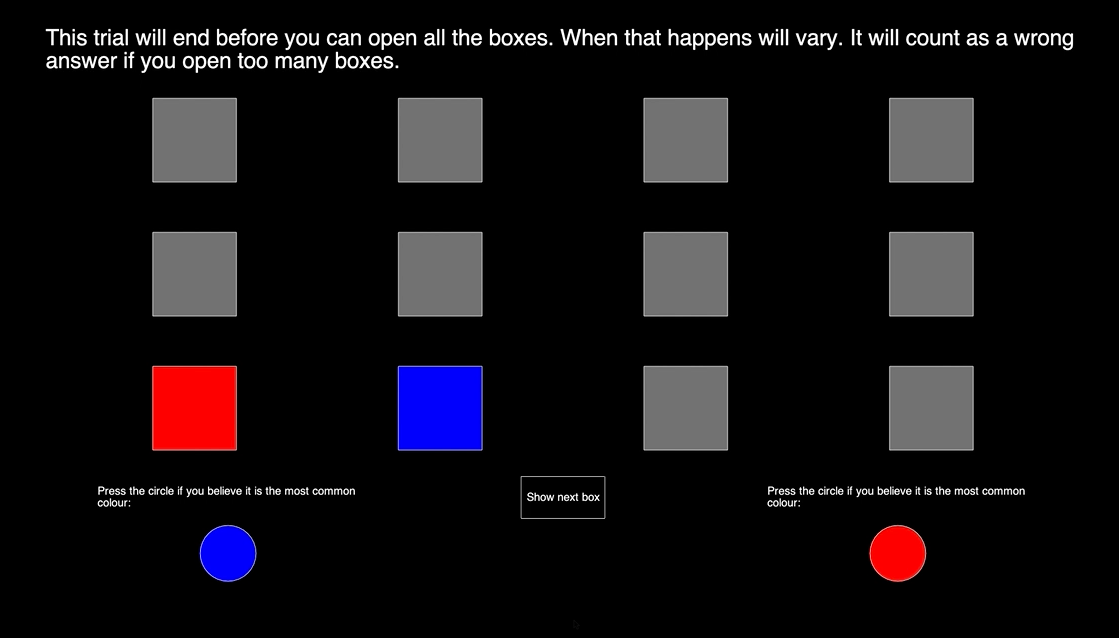
\includegraphics[scale=0.486]{Sections/Box task 2.png}
    \caption{Describe the figure}
    \label{picture_of_box_task}
\end{figure}

We have data from 76 participants that have done 10 trials each of the box task. The first trial was a practice trial of the limited version followed by three unlimited and six limited trials. We can model the decisions the participants make using a Softmax model, and fit this model to each participant with maximum likelihood estimation. Thus, we find the maximum likelihood estimates in the Softmax mode. Then, we find confidence intervals for each of these estimates using parametric bootstrapping and percentile intervals. 

As an input in the Softmax model we have an Ideal observer solution of the box task. An Ideal observer is a participant that always make optimal, or ideal, choices, and thus finds the best solution \citep{idealObs}. Each time a box is opened, the participant have three options. The first is to choose that blue is the majority colour, the second that red is, and the third option is to open another box. For each of these alternatives we have found loss functions, which represent the cost of choosing the different options. An Ideal Observer would always choose the alternative with the least loss, and would end up with the overall optimal or ideal solution. In this report we are assuming that the total number of red boxes is binomial distributed with parameters 12 and $\theta$. Each time a box is opened, the probability that the box is red is $\theta$ and $1-\theta$ that the box is blue. We also assume a beta prior for $\theta$ with parameters $\gamma$ and $\kappa$. If we have any prior beliefs about the probability of the different colours, this knowledge can be incorporated here. If both $\gamma$ and $\kappa$ is one, this is a uniform prior, meaning that $\theta$ has the same probability of being each possible value between zero and one. 



%(something about: here they are not said to answer when they are completely sure? compared to the beads task, where they are said to answer when comp sure. Jeg klarer ikke å finne ut hvor det står??)





%In this report we are firstly going to find an Ideal Observer solution of the box task. We assume that each time a box is opened, the probability that this box is red is $\theta$, and then that the probability that it is blue is $1-\theta$. We also choose a prior distribution for $\theta$, a beta distribution with parameters $\gamma$ and $\kappa$. If we have any prior beliefs about the probability of the different colours, this knowledge can be incorporated here. 
%Each time a box is opened, the participant have three options. The first is to choose that blue is the majority colour, the second that red is, and the third option is to open another box. For each of these alternatives we have found loss functions, which represent the cost of choosing the different options. An Ideal Observer would always choose the alternative with the least loss, and would end up with the overall best(?) solution. (should i say something about the fact that i have found another ideal observer solution assuming other things in the specialization thesis?)


% - We want to model how participants make decisions in the box task. We have data from 76 participants who have done 10 different trials of the box task, one practice trial that was limited, then followed by 3 unlimited and 6 limited trials. 
% - we can model this using a softmax model, and an Ideal Observer solution of the box task. From the specialization thesis we already have an Ideal observer solution assuming that the number of red boxes is uniformly distributed. 
% - three options each time a box is opened, loss functions for each option. An ideal observer always chooses the choice with the least loss. If we always do the best choice, we end up with the best solution.
%  - in this report we will also find another Ideal observer solution assuming a binomial distribution of the number of red boxes, and a beta prior for $\theta$. If we have beta(1,1), this will be a uniform prior. 

-paragraph about how this report is structured. 
\newpage
\chapter{Background Theory}
%\section{Theory}
In this chapter, we go through some of the statistical theory used in this report. This includes the theorem of total probability, Bayes' theorem, the beta and gamma functions, Bayesian modelling, loss functions, the law of total expectation, the softmax function, maximum likelihood estimation and bootstrapping.  

\section{The Theorem of Total Probability}
The theorem of total probability is often used when we want to find some probability, and this probability is hard to find. Then, sometimes it might be easier to find that probability if we condition on something, and use the theorem of total probability. 
\begin{theorem}[Theorem of Total Probability, Continuous Variables]
If we have a continuous variable, $\Theta$, and a discrete variable, $U$, and both $P(U=u|\Theta=\theta)$ and  $f_\Theta(\theta)$ are known for all $\theta$, then we can find $P(U=u)$ from \citep{schay2016introduction} 
\begin{equation}
    \label{lawoftotprob}
    P(U=u) = \int_{-\infty}^{\infty} P(U=u|\Theta=\theta)f_{\Theta}(\Theta=\theta) \: \dd \theta.
\end{equation}
\end{theorem}

\begin{comment}
In \citet{schay2016introduction}, the theorem of total probability for continuous variables is stated as 
\begin{theorem}[Theorem of Total Probability, Continuous Versions]
 For a continuous random variable Y and any event A, if $f_{Y|A}$ and $f_Y$ exists for all y, then
\begin{equation}
   % \label{lawoftotprob}
    P(A) = \int_{-\infty}^{\infty}
    P(A|Y=y)f_Y(y) dy.
\end{equation}
\end{theorem}
\end{comment}




Consider, for example, two discrete random variables $U$ and $V$ that are conditionally independent given the continuous stochastic variable $\Theta$. To find the probability that $U+V$ is equal to some integer $j$, we can use the theorem of total probability to condition on theta. Thus,
\begin{equation*}
    P(U+V=j) = \int_{-\infty}^\infty P(U+V=j|\Theta=\theta)f_{\Theta}(\Theta=\theta) \: d\theta.
\end{equation*}
Later, we can exploit the conditional independence. If $\theta$ is a probability defined on the interval (0,1), this will be integrated on that interval, such that 
\begin{equation*}
    P(U+V=j) = \int_{0}^1 P(U+V=j|\Theta=\theta)f_{\Theta}(\Theta=\theta) \: d\theta.
\end{equation*}
%Mer utfyllende her?




\section{Bayes' Rule}
We can use Bayes' rule to find conditional probabilities and distributions. 
\begin{theorem}[Bayes' Rule]
Consider two events, $A$ and $B$. We can find the probability of $A$ given event $B$ by the use of the probability of event $B$ given $A$ and the probabilities of the events $A$ and $B$ separately \citep{statinf}. Hence,
\begin{equation}
\label{bayesrule}
    P(A|B)=\frac{P(B|A)P(A)}{P(B)}.
\end{equation}
\end{theorem}


As an example, consider a discrete random variable, $U$. We can find the probability that $U$ is greater than or equal to 7, and condition on it being different from six by using \eqref{bayesrule}. Then $U \geq 7$ is an event, and $U\neq6$ is another event. Thus,
\begin{equation}
    P(U\geq 7|U\neq6) = \frac{P(U\neq6|U\geq7)P(U\geq7)}{P(U\neq6)}.
\end{equation}



\section{The Beta and Gamma Functions}
Later, we will use the beta and gamma functions and some of their properties. These are therefore stated here. This theory can for example be found in \citet{statinf}. The gamma function for a parameter $\kappa$ is 
\begin{equation*}
    \label{gamma_func}
    \Gamma(\kappa) = \int_0^\infty t^{\kappa-1}e^{-t} \dd t.
\end{equation*}
A useful property of the gamma function is that it is recursive. Hence,
\begin{equation}
\label{gamma_recursive_property}
    \Gamma(\kappa+1) = \kappa \Gamma(\kappa), \quad \kappa>0 .
\end{equation}

Additionally, the beta function with parameters $\gamma$ and $\kappa$ is defined as
\begin{equation}
\label{beta_function}
    \mathrm{B}(\gamma,\kappa) = \int_0^1 \theta^{\gamma-1}(1-\theta)^{\kappa-1} \: \dd \theta.
\end{equation}
We can express the beta function as a product of gamma functions. This yields
\begin{equation}
\label{beta_as_gamma}
    \mathrm{B}(\gamma,\kappa) = \frac{\Gamma(\gamma)\Gamma(\kappa)}{\Gamma(\gamma+\kappa)}.
\end{equation}



\section{Bayesian Modelling}
\label{theory_bayesian_modelling}
Consider a stochastic variable, $U$, that has a probability density function $f(u|\theta)$, where $\theta$ is a parameter upon which $U$ depends. In classical statistics, $\theta$ is said to be a fixed but unknown value. The goal is to find this one true value. 
However, in Bayesian statistics we consider $\theta$ as a stochastic variable, such that $\theta$ has a density function. 
Here, the goal is to find the underlying density. To do so we propose a prior distribution for $\theta$, $f(\theta)$. The prior distribution represents the prior knowledge we have about $\theta$ before observing any data. That could be our own subjective believes about the parameter or information based on other previously collected data or studies. One could also choose a prior distribution that does not say anything about the parameter at all. This is called a non-informative prior, and it is often used when we have none or little prior information about the parameter \citep{givens2012computational}. 
If we have collected data, denoted $u$, we can update our prior beliefs with the information we get from that data. The resulting distribution is called the posterior distribution of $\theta$, $f(\theta|u)$. We can find this using Bayes' theorem, and it includes both the prior information we have and the new information we get from the data. 

Consider a discrete stochastic variable, $U$, that has a sampling distribution $P(U=u|\theta)$, and let $P(U=u)$ be the marginal distribution of $U$. Additionally, let $f(\theta)$ be the prior distribution of $\theta$. Using Bayes' rule as it is stated in \eqref{bayesrule}, we get that the posterior distribution of $\theta$ given $u$, $f(\theta|u)$, can be expressed as \citep{statinf}
\begin{equation*}
    f(\theta|u) = \frac{P(U=u|\theta)f(\theta)}{P(U=u)}.
\end{equation*}
We can sometimes exploit the fact that the posterior distribution is proportional to the numerator in the above expression. This is because the denominator is a normalising constant. Hence,
\begin{equation}
    \label{posterior_proportional}
    f(\theta|u) \propto P(U=u|\theta)f(\theta).
\end{equation}
If \eqref{posterior_proportional} has the form of a known distribution, then that known distribution is the posterior distribution. 

As an example, consider a random variable, $U$, that is binomially distributed with parameters 12 and some probability, $\theta$. Thus,
\begin{equation*}
    \left( U|\Theta=\theta \right) \sim \mathrm{Binomial}(12,\theta).
\end{equation*}
Hence, the probability that we have $u$ successes out of twelve, given $\theta$, is
\begin{equation}
\label{binomial_12_ex}
    f(u|\theta) = \binom{12}{u} \theta^{u} (1-\theta)^{12-u}.
\end{equation}
As $\theta$ is a probability, its value is on the interval $[0,1]$. We know that the beta distribution is conjugate with the binomial distribution and has value between 0 and 1 \citep{statinf}, thus we choose a beta prior for $\theta$ with parameters $\gamma$ and $\kappa$. Hence,
\begin{equation}
\label{theta_with_beta_prior}
    \Theta \sim \mathrm{Beta}(\gamma,\kappa). 
\end{equation}
The prior density of $\Theta$ is then
\begin{equation}
    \label{betadistribution}
    f(\theta) = \frac{1}{\mathrm{B}(\gamma,\kappa)}\theta^{\gamma-1}(1-\theta)^{\kappa-1},
\end{equation}
where $B(\gamma,\kappa)$ is the beta function as defined in \eqref{beta_function}.
We can find the posterior distribution of $\theta$ using \eqref{posterior_proportional}, \eqref{binomial_12_ex} and \eqref{betadistribution}. Thus,
\begin{equation*}
    \begin{aligned}
        f(\theta|u) 
        &\propto f(u|\theta)f(\theta)\\[6pt]
        &\propto \binom{12}{u} \theta^{u} (1-\theta)^{12-u} \frac{1}{\mathrm{B}(\gamma,\kappa)}\theta^{\gamma-1}(1-\theta)^{\kappa-1}
    \end{aligned}
\end{equation*}
All the factors that do not include $\theta$ are constants, and we collect them together as one constant, denoted $C$. Then
\begin{equation*}
    \begin{aligned}
        f(\theta|u) 
        \propto C \: \theta^{u+\gamma-1}(1-\theta)^{12-u+\kappa-1}.
    \end{aligned}
\end{equation*}
We can see that this is proportional to a beta distribution like the one in \eqref{betadistribution}, but in this case with parameters $u+\gamma$ and $12-u+\kappa$. Hence, the posterior distribution is a beta distribution with these parameters, 
\begin{equation*}
    \Theta|U=u \sim \mathrm{Beta}(u+\gamma,12-u+\kappa).
\end{equation*}






\section{Loss Functions}
\label{theory_loss_functions}
A loss function typically says something about the cost, or loss, of an action related to a parameter. Let $\Omega_{\delta}$ be the action space, consisting of all the actions that we can do, where $\delta$ is an action. Then,
\begin{equation*}
    \delta \in \Omega_{\delta}.
\end{equation*}
Additionally, let $z$ be the true, but unknown state of nature, where 
\begin{equation*}
    z \in \Omega_z.
\end{equation*} 
We can define a loss function that depends on $z$ and $\delta$, which we denote $L(z,\delta)$. This is then the loss when making a decision, $\delta$, regarding $z$ \citep{statisticalDecisionTheoryLiese2008}.

A loss function could for example be the 0-1-loss function. If for example $\Omega_{\delta}= \Omega_z = \{0,1\}$, the loss function could be
\begin{equation}
\label{loss_func_indicator}
    L(z,\delta) = I(z \neq \delta),
\end{equation}
where $I$ is an indicator function such that
\begin{equation*}
    L(z,\delta) =
    \begin{cases}
        0,&  \text{if } z = \delta, \\
        1,&  \text{if } z \neq \delta.
    \end{cases}
\end{equation*}

In some cases, we would like to find the expected value of the loss function. Taking the expected value of an indicator function gives the probability that the event is happening \citep{algdat}. Hence, taking the expectation of \eqref{loss_func_indicator} gives
\begin{equation}
\label{expectation_of_loss_func_general}
    E[L(z,\delta)] = E[I(z\neq\delta)] = P(z\neq\delta).
\end{equation}



As an example, consider the box task with twelve boxes that could be either blue or red once they are opened. We define a stochastic variable, $X_i$, that represents the colour of the $i$-th opened box, such that 
\begin{equation}
\label{def_of_Xi}
    X_i =
    \begin{cases}
        0,& \text{if box }i \text{ is blue,}\\
        1,& \text{if box }i \text{ is red.}
    \end{cases}
\end{equation}
When $i$ boxes are opened, let $X_{1:i}$ denote the colours of the $i$ boxes, such that
\begin{equation}
\label{def_of_X1:i}
    X_{1:i} = (X_1,X_2,...,X_{i}).
\end{equation}
Additionally, let $Z$ be the colour that is in the majority when all twelve boxes are opened, the true majority colour. This is also a stochastic variable as it depends on the colours of the twelve boxes, the $X_i$'s. We define $Z$ as
\begin{equation}
\label{def_of_Z}
    Z = I\left(\sum_{j=1}^{12}X_j > 6\right).
\end{equation}
Then,
\begin{equation}
\label{Z_true_majority}
    Z = 
    \begin{cases}
        0,& \text{if blue is the true majority colour,} \\
        1,& \text{if red is the true majority colour.}
    \end{cases}
\end{equation}
Also, let $\delta$ be the choice the participant makes about which colour that is the dominant colour, such that
\begin{equation*}
    \delta = 
    \begin{cases}
        0,& \text{if the participant chooses blue as the majority colour,}\\
        1,& \text{if the participant chooses red as the majority colour}.
    \end{cases}
\end{equation*}
We can then define a loss function for the choice that the participant makes. This can be a 0-1 loss as in \eqref{loss_func_indicator}, and the loss function can therefore be defined as 
\begin{equation}
\label{loss_func_example}
    L(Z,\delta) = I(Z \neq \delta),
\end{equation}
Then, the loss is zero if the participant chooses the right colour as the majority colour and one if she chooses the wrong colour. 

To find the expected loss, we take the expectation of the loss function. As $Z$ depends on the colours of the twelve boxes, we condition on the colour of the already opened boxes, $ X_{1:i}=x_{1:i}$. The expectation of the loss function is then
\begin{equation*}
    E[L(Z,\delta)|X_{1:i}=x_{1:i}] = E[I(Z\neq \delta)|X_{1:i}=x_{1:i}].
\end{equation*}
As in \eqref{expectation_of_loss_func_general}, this expectation is the probability that $\delta \neq Z$, but here the probability depends on $X$. Thus,
\begin{equation}
\label{exp_loss_theory}
    E[L(Z,\delta)|X_{1:i}=x_{1:i}] = P(Z\neq \delta|X_{1:i}=x_{1:i}).
\end{equation}



%(Not sure if I should include this as this was fine when the loss func was if red or blue was teh right color, but now I have 3 decisions, and not two, and then teh 0-1-loss does not count, but it counts if we only talk about the two first decisions, decision 0 and 1.)





\section{The Law of Total Expectation}
Let $\{A_1,A_2,...,A_k\}$ be a partition of the sample space, $S$. Thus, there are $k$ non-overlapping parts, such that $A_i \cap A_j = \emptyset$, $\forall \:
i \neq j$. Then we also have that $S = A_1 \cup A_2 \cup...\cup A_k$. If we want to find the expectation of an event, $B$, and we have the expectation of $B$ on each of these partitions, we can use the law of total expectation. It states that
\begin{equation}
    E[B] = \sum_i E[B|A_i]P(A_i).
\end{equation}
This can also be used to find the expectation of functions \citep{schay2016introduction}. Let $g(B)$ be the function that we want to take the expectation of, then
\begin{equation}
\label{law_tot_exp_func}
    E[g(B)] = \sum_i E[g(B)|A_i]P(A_i).
\end{equation}

Later we will use the law of total expectation when we find the expectation of a loss function that says something about the loss of opening the next box in the box task. This expected loss is dependent on the colour of the box that will be opened. Thus, to find that expected loss, we use the law of total expectation and condition on the colour of the following box. 

%Again consider the box task. Let $\delta_i=2$ denote the choice of opening another box when $i$ boxes already are opened. We can in addition to the loss functions found above, \eqref{loss_func_example}, find a loss function for the choice of opening the next box. This loss function is dependent on the choice that are made after the next box is opened as well. We denote these as $\delta_{(i+1):12}$, and thus, we denote this loss function as $L(Z,\delta_i=2,\delta_{(i+1):12})$ (senere kaller jeg disse videre valgene for $IO(\textbf{x}_{i},0)$, men det blir litt mange greier å ta med her. hva skal jeg gjøre md det?). 

%The expectation of this loss function is dependent on the colour of the next box, $X_{i+1}$. We do not know the colour of that box, but we can find probabilities for the box being blue and red given the colour of the first $i$ boxes, $P(X_{i+1}=0|\textbf{x}_i)$ and $P(X_{i+1}=1|\textbf{x}_i)$, respectively. We can then find the expectation of this loss function using \eqref{law_tot_exp_func}, and condition on $X_{i+1}$. Then, 
%\begin{equation*}
%    E[L(Z,\delta_i=2,\delta_{(i+1):12})|\textbf{x}_i] = \sum_{j=0}^1
%    E[L[Z,\delta_{(i+1):12}|\textbf{x}_i]P(X_{i+1}=j|\textbf{x}_i).
%\end{equation*}
%Er dette litt mye greier å ta med her? Feks mtp notasjonen. Og er notasjonen godt nok forklart her?






\section{The Softmax Function} \label{section_theory_softmax}
The softmax function is commonly used in classification problems with more that two classes \citep{softmax}. Consider a decision, $\Delta$, which now is a stochastic variable for which we want to construct a distribution. We find a probability mass function for $\Delta=\delta$ using a softmax function. Let there be $D$ decisions, such that
\begin{equation*}
    \delta \in \{0,1,2,...,D-1\}.
\end{equation*}
Additionally, let $\EE_{\delta}(\vp)$ be values tied to each decision that depends on some parameters, $\vp$. The probability mass function for each decision, $\delta$, could be found using a softmax function, such that
\begin{equation}
\label{softmax_in_theory}
    \begin{aligned}
        f(\delta|\vp,\eta) = \frac{\text{exp}(- \eta \EE_{\delta}(\vp))}{\sum_{d=0}^{D-1} \text{exp}(-\eta \EE_{d}(\vp))},
    \end{aligned}
\end{equation}
where $\eta$ is some parameter. 

These decisions could, for example, be the three choices we have each time we open a box in the box task. These choices are that blue is the majority colour, or that red is, denoted $\delta=0$ and $\delta=1$, respectively. The last choice is to open another box, which we denote $\delta=2$. Then, we let $\EE_0(\vp)$ be the expected loss when choosing that blue is the majority colour, similarly to \eqref{exp_loss_theory}. Additionally, we let $\EE_1(\vp)$ and $\EE_2(\vp)$ be the expected loss of choosing red as the majority colour and of opening another box, respectively. Then, the probability mass function for $\delta$ could be as in \eqref{softmax_in_theory}. We then have a probability mass function for each of the three decisions that depend on the expected losses, parameters $\vp$ and some parameter $\eta$.




\section{Maximum Likelihood Estimation}
\label{section_theory_mle}

Maximum likelihood estimation is used to find estimates for parameters in a distribution. These are the estimates that, as the name implies, maximises the likelihood, and for short, we call them MLEs. Assume that we have probability distribution for a stochastic variable, $\Delta$, and consider $n$ samples, $\delta_1,\delta_2,...,\delta_n$, of $\Delta$. Denote the probability mass function for each of these $\delta$'s as $f(\delta|\vp)$, where $\vp$ contains the parameters in the probability mass function. If the $\delta_i$'s are independent, the likelihood function is defined as
\begin{equation}
\label{likelihood}
    L(\vp|\delta_1,\delta_2,...,\delta_n) =  \prod_{i=1}^{n} f(\delta_i|\vp).
\end{equation} 
The MLEs are then the estimates of $\vp$ that maximises this function, and they are usually denoted $\hat{\vp}$. It is often hard to maximize the likelihood function, then it might be easier to take the logarithm of the likelihood function and maximize that instead. This is called the log likelihood function, and is normally denoted as $l$. Thus,
\begin{equation}
\label{chap2:log_likelihood}
    \begin{aligned}
        l(\vp|\delta_1,\delta_2,...,\delta_n) 
        =& \text{log}\left(L(\vp|\delta_1,\delta_2,...,\delta_n)\right)\\
        =& \text{log}\left(\prod_{i=1}^{n} f(\delta_i|\vp) \right).
    \end{aligned}
\end{equation}
As the logarithm of products is the sum of the logarithms, we get that the log likelihood is
\begin{equation}
\label{chap2:log_likelihood2}
    \begin{aligned}
        l(\vp|\delta_1,\delta_2,...,\delta_n) = \sum_{i=1}^n \text{log}(f(\delta_i|\vp)).
    \end{aligned}
\end{equation}
Maximizing this will give the same maximum point as if we maximize the likelihood function \citep{statinf}. 

As an example, consider that the $\delta_i$'s have probability mass function as in \eqref{softmax_in_theory}. The parameters that we want to find estimates for are then $\vp$ and $\eta$. If we have $n$ samples of $\Delta$, denoted $\delta_i$, where $i \in \{1,2,...,n\}$,
the likelihood function would be
\begin{equation*}
    \begin{aligned}
        L(\vp,\eta|\delta_1,\delta_2,...,\delta_n) 
        =& \prod_{i=1}^{n} f(\delta_i|\vp,\eta)\\[6pt]
        =& \prod_{i=1}^{n}
        \frac{\text{exp}(- \eta \EE_{\delta_i}(\vp))}{\sum_{d=0}^{2} \text{exp}(-\eta \EE_{d}(\vp))}.
    \end{aligned}
\end{equation*}
The log likelihood would then be
\begin{equation*}
    \begin{aligned}
        l(\vp,\eta|\delta_1,\delta_2,...,\delta_n) =& \sum_{i=0}^N \text{log}\left( \frac{\text{exp}({-\eta \EE_{\delta_{i}}(\vp))}}
        {\sum_{d=0}^{2} \text{exp}(-\eta \EE_{d}(\vp))}\right) \\[6pt]
        =& \sum_{i=0}^N \left(
        -\eta \EE_{\delta_{i}} 
        - \text{log} \left( \sum_{d=0}^{2} \text{exp} \left(-\eta \EE_{d}(\vp)\right) \right) \right).
    \end{aligned}
\end{equation*}
The maximum likelihood estimators of $\vp$ and $\eta$ would then be the values that maximises this log likelihood function. We denote them as $\hat{\vp}$ and $\hat{\eta}$.




\section{Bootstrapping}
\label{section_theory_bootstrap}
Consider a sample, $(\delta_1,\delta_2,...,\delta_n)$, where the $\delta_i$'s are identically and independently distributed from an unknown distribution, $F$. We can use this sample to estimate this distribution, denoted by $\hat{F}$. To get some ideas about the properties of $F$, we can find the properties of $\hat{F}$. Sometimes it is challenging to do this analytically. Instead, we can use simulations, and this is where bootstrapping is useful. Bootstrapping is a way of finding new samples, either from the original sample, $(\delta_1,\delta_2,...,\delta_n)$, or from the estimated distribution, $\hat{F}$. We can then use those samples to find, for example, standard error, bias, variance, or perhaps the most common; confidence intervals \citep{bootstrap}.


%a sample (iid) from an unknown distribution ($F$). can use that sample to estimate the distribution, hence find $\hat{F}$. To get some knowledge about the properties of $F$, we can find out things about the properties of $\hat{F}$. Often hard to do this analytically, thus, instead we use simulations. Then we can use bootstrapping. 


%Bootstrapping is a way of doing statistical inference using samples from a dataset. It can be used to measure the accuracy of parameters. We can for example find standard errors, bias, variance, or perhaps the most common, confidence intervals. In that way we do not need any formulas, only many samples \citep{bootstrap}. However, with many samples, we are dependent on a computer. 

There are two types of bootstrapping, nonparametric and parametric. In the nonparametric bootstrap, $\hat{F}$ is the empirical distribution of the data, and we take samples from our original sample. Consider for example that you have a dataset, $\boldsymbol{\delta}=(\delta_1,\delta_2,\delta_3,\delta_4,\delta_{5})$. A bootstrap sample of this might then be $(\delta_5,\delta_5,\delta_2,\delta_3,\delta_1)$ and another might be $(\delta_2,\delta_{4},\delta_{2},\delta_{2},\delta_{1})$. These are resampled versions of $\boldsymbol{\delta}$. Thus, the bootstrap samples consists of elements from the original dataset, but some of them might not appear at all in a bootstrap sample while others might appear more than once. Drawing $B$ of these samples, we can do inference about the population the original data is from. 

In the parametric bootstrap, we make assumptions about the population, and $\hat{F}$ is the parametric distribution. Consider a sample, ($\delta_1,\delta_2,...,\delta_n$), from a distribution that has a probability mass function $f(\delta|\vp)$, where $\vp$ might be a vector of parameters \citep{statinf}. We can for example find an estimate, $\hat{\vp}$, of $\vp$, using maximum likelihood estimation as in Chapter \ref{section_theory_mle}. When we have done that, we can draw new samples, denoted $\delta_i^*$ from $f(\delta|\hat{\vp})$, such that
\begin{equation*}
    \delta_1^*,\delta_2^*,...,\delta_n^* \sim f(\delta|\hat{\vp}).
\end{equation*}
If we draw $B$ samples, we can, as for the nonparametric bootstrap, do inference. 



%Bootstrapping is a way to draw or simulate many samples from one single dataset. If you have a dataset, you can draw random samples from them with replacement, to construct bootstrap samples \citep{bootstrap}. If you for example have data $\textbf{x}=(x_1,x_2,x_3,x_4,x_{5})$, then a bootstrap sample might be $(x_5,x_5,x_2,x_3,x_1)$ and another might be $(x_2,x_{4},x_{2},x_{2},x_{1})$. These are then resampled versions of $\textbf{x}$. Thus, the bootstrap samples consists of elements from the original dataset, but some of them might not appear at all in a bootstrap sample while others might appear more than once. This is called nonparametric bootstrapping. If we, for example, have found the maximum likelihood estimate (MLE) of a parameter, $\eta$, we can use these bootstrap samples to for example find the standard error or confidence interval (CI) for $\eta$.

%If we have a distribution for the $x$'s, we could instead of using a nonparametric bootstrapping, use a parametric version. Then we simulate new $x$'s based on the MLE of $\eta$. If the distribution is $f(x|\eta)$, and the MLE of $\eta$ is denoted $\hat{\eta}$, then we simulate new $x$'s with $f(x|\hat{\eta})$, and get new samples, $(\hat{x}_1,\hat{x}_2,\hat{x}_3,\hat{x}_4,\hat{x}_5)$. As for the nonparametric bootstrap, we can simulate many samples, and for example find standard errors and confidence intervals (CIs) for parameters. 

\subsection{Confidence Intervals with Bootstrap Samples}
\label{theory_ci_bootstrap}
One way of doing inference is to find confidence intervals. When we have $B$ bootstrap samples, there are multiple methods for finding these.  
A confidence interval (CI) for a parameter is an interval that will contain the true value of the parameter a given proportion of the times an interval is constructed. If we, for example, have a 90\% CI, then the true value of the parameter will be in the interval 90\% of the times we construct a new one \citep{bootstrap}.

One method for finding CIs with bootstrap samples is the percentile method. The percentile method is simple to both understand and implement. However, these confidence intervals might be biased. Then, one could instead use approaches such as \textit{bias corrected and accelerated} intervals or \textit{approximate bootstrap confidence} intervals. In this report, we use the percentile method to find confidence intervals. 

Consider a situation with $B$ bootstrap samples. Let the vector $\vp$ be a parameter, for which we want to find a confidence interval. Then, we find the MLE of $\vp$ for each of the $B$ samples.
If we want to find a 90\% confidence interval using the percentile method, we find the 5-th and 95-th percentiles. 
Plotting the MLEs of $\vp$ is a histogram, the 5-th percentile is the value of $\hat{\vp}$ in the histogram where 5\% of the samples are below. The 95-th is where 5\% of the values are above. This is visualised in Figure \ref{percentile_ci_example}. Here we have 150 bootstrap samples, and we have found the MLE of $\vp$ for each sample. These values are plotted in a histogram, where the red dashed lines represent the 5-th and 95-th percentiles. Then 5\% of the MLEs lie to the left of the left red line, and 5\% lie to the right of the right red line. The 90\% CI for $\vp$ is around (1.4,7) when using the percentile method.
\begin{figure}
    \centering
    %\includegraphics{}
    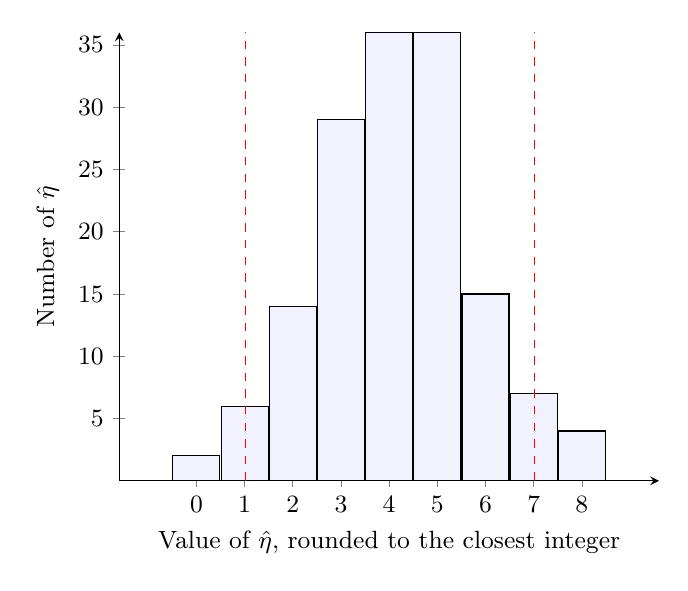
\begin{tikzpicture}[font=\small]
\begin{axis}[
ybar,
bar width=17pt,
xlabel={Value of $\hat{\eta}$, rounded to the closest integer},
ylabel={Number of $\hat{\eta}$},
ymin=0,
ytick={5,10,15,20,25,30,35,40},
xtick=data,
axis x line=bottom,
axis y line=left,
enlarge x limits=0.2,
]
\addplot[fill=myblue] coordinates {
    (0,2)
    (1, 6)
    (2, 14)
    (3, 29)
    (4, 36)
    (5, 36)
    (6, 15)
    (7, 7)
    (8, 4)
};
\end{axis}
\draw[dashed,red](1.6,0) -- (1.6,5.7);
\draw[dashed,red](5.27,0) -- (5.27,5.7);
\end{tikzpicture}
    \caption[Bootstrap Example]{Here we have plotted the MLEs of 150 bootstrap samples in a histogram. The red dashed lines represent the 5-th and 95-th percentiles.}
    \label{percentile_ci_example}
\end{figure}

\newpage
%\section{Problem Setup}
\chapter{Model formulation}
\label{Chapter_Problem_setup}
%Describe the box task, both versions. 
The box task is an information sampling task that is used to assess a 'jumping to conclusions' (JTC) bias \citep{balzan2017}. In the box task used in this report the participants are shown a grid of twelve boxes, and each time a box is opened, one out of two colours, for example blue or red, is displayed. The participants are told that one of the colours is always in majority, and that their task is to find out which one. We are using two different versions of the box task. In the first one the participant can open as many of the twelve boxes as they want before deciding which of the two colours that is in majority. We call this the unlimited version. In the second one, which we call the limited version, the participants are told that the test will terminate at one point when a random box is opened. If the participant have not decided what the majority colour is when the test terminates, this counts as a failed trial. 

We have data from 76 participants that have done multiple trials of both versions of the box task. The experiment where the data was collected was carried out by Professor Gerit Pfuhl and Doctoral Research Fellow Kristoffer Klevjer at UiT The Arctic University of Norway in February 2020. The participants were recruited from an undergraduate psychology course. They did a practice limited trial first that terminated after three boxes where opened, such that if they tried to open a fourth box, the test terminated, and they were not able to make a decision. That trial is not analyzed here. Following the practice trial where three unlimited trials. The participants could in these trials open as many of the twelve boxes as they wanted before deciding on what they think is the dominant colour. Lastly, there where six limited trials. Three of them terminated after six boxes had been opened and the other three terminated after nine boxes had been opened. These are the trials we analyze, thus we analyze Trials 2 to 10. We have data for how many boxes each participant has opened in each of the nine trials. We call this 'draws to decision'. The participants have either opened boxes until they have decided what they think is the majority colour or until the test terminates, and we have data for what they chose, or whether the test terminated before they were able to choose. To compensate for possible biases towards one colour, the two colours where changed for each new trial. They could for example be green and pink in the first trial and blue and yellow in the second trial. For simplicity, we are in this report referring to these colour as blue and red for all trials.

For each trial there is a fixed sequence of boxes. The participants are only able to choose whether to open the next box or not, not which box that opens. Thus, we know how many of the boxes that were blue and how many that were red for each step in the trials. In Figure \ref{fig:trial2_order}, we see the order the boxes are opened in in Trial 2, which is an unlimited trial. In Figure \ref{fig:histogram_trial2}, the draws to decisions for all participants are shown in a histogram. Here, the number of boxes that are opened when the participant chooses what he thinks is the majority colour is on the horizontal axis. On the vertical axis are the number of participants that has chosen on that particular box. We see that many participants have chosen majority colour after three boxes are opened. All of these three boxes are red, thus, there is a high probability that red is the dominant colour. 
As the participants are told that one of the colours always is in majority, we can be completely sure if six of the opened boxes are red, that red is the dominant colour. This is because there cannot be six of each box if one of them is in majority. When seven boxes are opened in Trial 2, six of them are red, and we know then that red is the dominant colour. Seven participants have chosen colour after seven boxes are opened. Some participants wait longer, even though they can be completely sure after seven boxes are opened.
\begin{figure}
    \centering
    \scalebox{0.8}{\begin{tikzpicture}[node distance = 1.2cm]
    \node (1) [red_trial]{}; 
    \node (2)[red_trial, right of=1]{};
    \node (3)[red_trial, right of=2]{};
    \node (4)[blue_trial, right of=3]{};
    \node (5)[red_trial, right of=4]{};
    \node (6)[red_trial, right of=5]{};
    \node (7)[red_trial, right of=6]{};
    \node (8)[red_trial, right of=7]{};
    \node (9)[blue_trial, right of=8]{};
    \node (10)[red_trial, right of=9]{};
    \node (11)[blue_trial, right of=10]{};
    \node (2)[red_trial, right of=11]{};
\end{tikzpicture}}
    %\includegraphics{}
    \caption[Order of Boxes in Trial 2]{The order of the boxes in Trial 2. This is an unlimited trial.}
    \label{fig:trial2_order}
\end{figure}


\begin{figure}
    \centering
    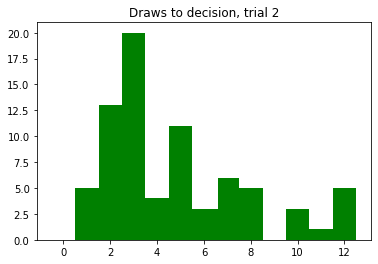
\includegraphics[scale=0.6]{pictures/dtd2_histogram.png}
    \caption[Draws to Decisions in Trial 2]{Histogram of the draws to decisions for all participants in Trial 2. 
    har forandret på denne figurern, husk å bytte til riktig!!}
    \label{fig:histogram_trial2}
\end{figure}


In Trial 3, which also is an unlimited trial, it takes more boxes to be completely sure what the majority colour is. As shown in Figure \ref{fig:trial3_order}, there are six blue boxes when ten of the boxes are opened. We see in Figure \ref{fig:histogram_trial3} that the participants in general open more boxes before choosing the majority colour in this trial than in Trial 2. 

\begin{figure}
    \centering
    \scalebox{0.8}{\begin{tikzpicture}[node distance = 1.2cm]
    \node (1)[blue_trial]{}; 
    \node (2)[red_trial, right of=1]{};
    \node (3)[blue_trial, right of=2]{};
    \node (4)[red_trial, right of=3]{};
    \node (5)[blue_trial, right of=4]{};
    \node (6)[blue_trial, right of=5]{};
    \node (7)[red_trial, right of=6]{};
    \node (8)[blue_trial, right of=7]{};
    \node (9)[red_trial, right of=8]{};
    \node (10)[blue_trial, right of=9]{};
    \node (11)[red_trial, right of=10]{};
    \node (2)[blue_trial, right of=11]{};
\end{tikzpicture}}
    %\includegraphics{}
    \caption[Order of Boxes in Trial 3]{The order of the boxes in Trial 3. This is an unlimited trial.}
    \label{fig:trial3_order}
\end{figure}

\begin{figure}
    \centering
    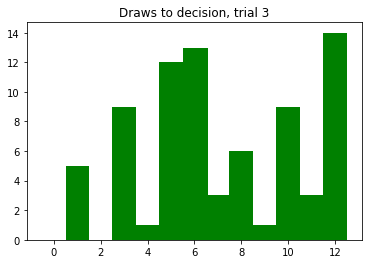
\includegraphics[scale=0.6]{pictures/dtd3_histogram.png}
    \caption[Draws to Decisions in Trial 3]{Histogram of the draws to decisions for all participants in Trial 3. 
    har forandret på denne figurern, husk å bytte til riktig!!}
    \label{fig:histogram_trial3}
\end{figure}

Both Trial 5 and Trial 8 are limited trials that terminates after nine boxes are opened. The order of the boxes in Trial 5 is shown in Figure \ref{fig:trial5_order}. When seven boxes are opened, six of them are blue, and we can therefore conclude when seven boxes are opened that blue is the majority colour. We see in Figure \ref{fig:histogram_trial5} that many participants chooses majority colour after three boxes are opened, when there are only blue boxes. In Trial 8 there are never two boxes of the same colour following each other, as shown in Figure \ref{fig:trial8_order}. There are never six of one of the colours, meaning that we never can be completely sure which one is the majority colour. This is reflected in the draws to decision for the participants, as shown in Figure \ref{fig:histogram_trial8}. We see that the test terminates for many of the participants before they are able to choose what they think is the majority colour. 
\begin{figure}
    \centering
    \scalebox{0.8}{\begin{tikzpicture}[node distance = 1.2cm]
    \node (1)[blue_trial]{}; 
    \node (2)[blue_trial, right of=1]{};
    \node (3)[blue_trial, right of=2]{};
    \node (4)[red_trial, right of=3]{};
    \node (5)[blue_trial, right of=4]{};
    \node (6)[blue_trial, right of=5]{};
    \node (7)[blue_trial, right of=6]{};
    \node (8)[blue_trial, right of=7]{};
    \node (9)[red_trial, right of=8]{};
\end{tikzpicture}}
    \caption[Order of Boxes in Trial 5]{The order of the boxes in Trial 5. This is a limited trial that terminates after nine boxes are opened.}
    \label{fig:trial5_order}
\end{figure}
\begin{figure}
    \centering
    \scalebox{0.8}{\begin{tikzpicture}[node distance = 1.2cm]
    \node (1)[blue_trial]{}; 
    \node (2)[red_trial, right of=1]{};
    \node (3)[blue_trial, right of=2]{};
    \node (4)[red_trial, right of=3]{};
    \node (5)[blue_trial, right of=4]{};
    \node (6)[red_trial, right of=5]{};
    \node (7)[blue_trial, right of=6]{};
    \node (8)[red_trial, right of=7]{};
    \node (9)[blue_trial, right of=8]{};
\end{tikzpicture}}
    \caption[Order of Boxes in Trial 8]{The order of the boxes in Trial 8. This is a limited trial that terminates after nine boxes are opened.}
    \label{fig:trial8_order}
\end{figure}
\begin{figure}
    \centering
    \begin{minipage}{0.45\textwidth}
        \centering
        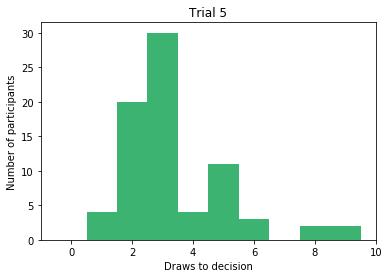
\includegraphics[scale=0.4]{pictures/dtd5_histogram.png}
        \caption[Draws to Decisions in Trial 5]{The draws to decisions for all participants in Trial 5. That is, how many boxes they open before they choose what they think is the majority colour, of before the test terminates.}
        \label{fig:histogram_trial5}
    \end{minipage}\hfill
    \begin{minipage}{0.45\textwidth}
        \centering
        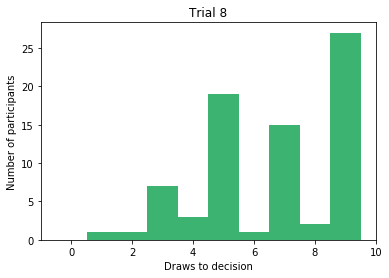
\includegraphics[scale=0.4]{pictures/dtd8_histogram.png}
        \caption[Draws to Decisions in Trial 8]{The draws to decisions for all participants in Trial 8. That is, how many boxes they open before they choose what they think is the majority colour, of before the test terminates.}
        \label{fig:histogram_trial8}
    \end{minipage}
\end{figure}

The order of the boxes for all trials can be found in Appendix \ref{appendix_a}. Here we also have histograms of the draws to decision for all of the trials.

In the following, we formulate a model for how decisions are made in the box task, and we find parameter estimates such that we can fit the model to each person. We also find a so-called Ideal Observer solution of the box task. An Ideal Observer would always make optimal decisions \citep{idealObs}. Thus, an Ideal Observer solution is close to an optimal solution of the box task. 



\section{Modelling Framework}
\label{section_notation}
Before we start with the formulation of the model, we will introduce some notation and present some assumptions. 

Let $X_i$ be the colour of the $i$-th opened box. If the box is blue, $X_i$ is 0 and if the box is red, $X_i$ is one. Thus,
\begin{equation*}
    X_i = \begin{cases}
    0,& \quad \text{if box } i \text{ is blue,}\\
    1,& \quad \text{if box } i \text{ is red.}
    \end{cases}
\end{equation*}
We assume that each $X_i$ has a Bernoulli distribution with success probability $\theta$, where we later condition on there not being six blue and six red boxes. Then,
\begin{equation*}
    X_i \sim \text{Bernoulli}(\theta).
\end{equation*}
We define a vector, $X_{1:i}$, that contains the colours of the first $i$ boxes that are or will be opened, such that $X_{1:i} = (X_1,X_2,...,X_{i})$. In the same way, we let $x_{1:i} = (x_1,x_2,...,x_{i})$.

Additionally, let $U_i$ be the number of the first $i$ opened boxes that are red. Thus, $U_i$ is a stochastic variable defined as
\begin{equation}
\label{def_of_U}
    U_i = \sum_{j=1}^{i} X_j. 
\end{equation}
The sum of Bernoulli distributed variables is binomially distributed \citep{statinf}. Thus, $U_i$ is binomially distributed with parameters $i$ and $\theta$. We define another stochastic variable, $V_i$, that is the number of red boxes that are not opened when $i$ boxes are opened. Thus, $V_i$ is the number of red boxes out of the $12-i$ boxes that are not opened, which yields,
\begin{equation}
\label{def_of_V}
    V_i = \sum_{j=i+1}^{12} X_j.
\end{equation}
This variable is also binomially distributed, but with parameters $12-i$ and $\theta$. Thus,
\begin{equation}
\label{U_V_binomal_distri}
    \begin{aligned}
        U_i &\sim \text{Binomial}(i,\theta)\\
        V_i &\sim \text{Binomial}(12-i,\theta).
    \end{aligned}
\end{equation}
%\begin{subequations}
%\begin{equation}
%\label{U_binomail_distr}
%    U_i \sim \text{Binomial}(i,\theta)
%\end{equation}
%\begin{equation}
%\label{V_binomial_distr}
%    V_i \sim \text{Binomial}(12-i,\theta).
%\end{equation}
%\end{subequations}
Then, we have that 
\begin{equation}
\label{ui_prob_mass}
    P(U_i=u_i|\Theta=\theta) = \binom{12}{u_i} \theta^{u_i}(1-\theta)^{12-u_i},
\end{equation}
and
\begin{equation}
\label{vi_prob_mass}
    P(V_i=v_i|\Theta=\theta) = \binom{12-i}{v_i} \theta^{v_i}(1-\theta)^{12-i-v_i}.
\end{equation}

Just as in Chapter \ref{theory_bayesian_modelling}, we let $\Theta$ have a conjugate beta prior with parameters $\gamma$ and $\kappa$, as shown in \eqref{theta_with_beta_prior}.
The prior distribution of $\Theta$ is then as given in \eqref{betadistribution}.

Figure \ref{fig:pdf_beta_distr} shows the probability density function of the beta distribution for different values of $\gamma$ and $\kappa$. The pink line represents the situation where $\gamma=\kappa=1$. This is the same as a uniform prior for $\theta$. That means that the probability of $\theta$ being anywhere on the interval between 0 and 1, is constant. As the participants are told that one of the colours will be in majority, but get no information about which one, this might be a suitable prior.
However, one might argue that our prior beliefs resembles more the purple or orange lines as we know that one of the colours will definitively be in majority, thus it is not really reasonable to assume that $\theta$ is 0.5. For this reason we also exclude all priors that have $\gamma$ and $\kappa$ larger than 1, which is the situation for the black and grey lines. 

\begin{figure}
    \centering
    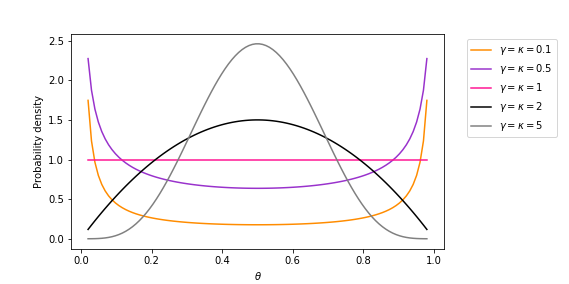
\includegraphics[scale=0.5]{pictures/beta_pdf.png}
    \caption[Probability Density for the Beta Distribution]{The probability density function for the beta distribution plotted for different values of the hyperparameters $\gamma$ and $\kappa$.}
    \label{fig:pdf_beta_distr}
\end{figure}


Of all the 12 boxes, $U_i+V_i$ is the total number of red boxes.
Consequently, if $U_i+V_i$ is bigger than 6, it is a red majority in the box task, and if it is smaller than 6, the true majority colour is blue. We denote this true majority colour as $Z$, such that
\begin{equation}
\label{def_of_Z_2}
    Z = I(U_i+V_i>6).
\end{equation}
This is the same as defining $Z$ as in \eqref{def_of_Z}, as $U_i+V_i = \sum_{j=1}^{12}X_j$, and the order that the boxes are opened in does not affect the majority. Then, as in \eqref{Z_true_majority}, $Z$ is 0 if the true majority colour is blue and 1 if the true majority colour is red. 


%Each time a box is opened, we have three choices. The first is to choose that blue is the majority colour, the second that red is and the third is to open another box. Let $\delta_{i+1}$ denote the different choices when $i$ boxes are opened. If $\delta_{i+1}=0$, we have chosen that blue is the majority colour, $\delta_{i+1}=1$ shows that red is chosen as the majority and $\delta_{i+1}=2$ represents the choice of opening the next box, which is box $i+1$. Moreover, let $\delta_{(i+2):12}$ be the choices made after box $i+1$ is opened. 

Each time a box is opened, the participants have three choices. The first is to choose that blue is the dominant colour, the second that red is, and the third is to choose to open another box. We denote these decisions as $\delta_i$, where $i$ is the number of boxes that are opened. If $\delta_i = 0$, the participant chooses that blue is the more prominent colour, thus that there are in total, of all twelve boxes, more blue boxes than red. Moreover, $\delta_i=1$ means that the participant has chosen that red is the dominant colour, and $\delta_i=2$ represents the situation where the participant chooses to open the next box. Thus,
\begin{equation}
\label{def_of_delta}
    \delta_i =
    \begin{cases}
        0,& \quad \text{if blue is chosen as majority colour,}\\
        1,& \quad \text{if red is chosen as majority colour,}\\
        2,& \quad \text{if the participant chooses to open the next box.}
    \end{cases}
\end{equation}
%We denote the choices that are made from when $i$ boxes are opened to the last choice is made as $\delta_{i:12}$. Something about not making decisions after majority colour is chosen, such that for example $\delta_{12}$ might not exist. dette trgner jeg ikke hvis jeg isf bruker IO(\textbf{x}$_i,\delta_{i+1}$).

We can define loss functions for each of these decisions. These loss functions depend on the true majority colour, $Z$, and the decision that is made, $\delta_i$. Similarly to Chapter \ref{theory_loss_functions}, we denote the loss function when $i$ boxes are opened as $L_i[Z,\delta_i;\vp]$. In our case, we have that 
\begin{equation*}
    \Omega_Z = \{0,1\}
\end{equation*}
and 
\begin{equation*}
    \Omega_{\delta_i}=\{0,1,2\}.
\end{equation*}
%$\Omega_Z = \{0,1\}$ and $\Omega_{\delta_i}=\{0,1,2\}$.


If we take the expectation of this loss function, we get the expected loss for each of these decisions when $i$ boxes are opened, which we denote
\begin{equation*}
    \EE^i_{\delta_i}(\vp) = E\left[ L_i[Z,\delta_i;\vp|X_{1:i}=x_{1:i}]\right],
\end{equation*}
as it depends on some parameters $\vp$. This expected loss also depends on the colours of the $i$ boxes that already are opened, $x_{1:i}$.

In the limited version of the box task, the participants are told that the test will terminate when a random box is opened. Thus, we need a random variable that represents how many boxes that are open when the test terminates. We call this variable $T$. If $T=3$, then the participant has opened three boxes and wants to open the fourth when the test terminates. Then, instead of seeing the colour of the fourth box, the test terminates, and this is a failed trial. The information given to the participants regarding this is that the test will terminate when a random box is opened. We assume that the first box always can be opened, but that the probabilities that the test terminates at the subsequent boxes are the same. When 12 boxes are opened, there are no more boxes to open, thus, no more chances for the test to terminate. Thus, $T$ is uniformly distributed with on $\{1,2,3,4,5,6,7,8,9,10,11\}$, 
\begin{equation}
\label{T_uniform}
    T \sim \text{Uniform}(\{1,2,3,4,5,6,7,8,9,10,11\}).
\end{equation}

Now we have all the notation needed to define the model for how the participants make decisions. 

\section{The Model for Decisions/something else}
Having the notation for the expected losses and decisions, we can define the probability mass function for the decisions using a softmax function similar to the one in \eqref{softmax_in_theory}. 

For each participants we have observed decisions, $\boldsymbol{\delta}=(\delta_1,\delta_2,...,\delta_n)$, where $\delta_j \in \{0,1,2 \}$ as in \eqref{def_of_delta}, and $n$ is the total amount of decisions we have for each participant. Thus, $j\in \{1,2,...,n \}$. As the participants have opened a different amount of boxes each time, $n$ varies form participant to participant. Recall that $i$ is the number of boxes that are opened, and that $i$ is reset for each new trial. Thus, the probability mass function for the decisions can be expressed as
\begin{equation}
\label{softmax_theta}
    f(\delta_{j}|\vp,\eta;x_{1:i}) = \frac{\text{exp}(- \eta \EE^i_{\delta_{j}}(\vp))}{\sum_{d=0}^{2} \text{exp}(-\eta \EE^i_{d}(\vp))},
\end{equation}
where $\eta$ is some parameter. This can be interpreted as a measure of how far the choices the participants make are away from the decision with the least expected loss. If $\eta$ is infinity, they always make the decision with the lowest expected loss, and if $\eta$ is zero, they choose arbitrarily. A negative value of $\eta$ indicates that the participant tends to choose the decisions with higher expected losses.


When we have this model, we can find estimates of the parameters $\theta$ and $\eta$ for each participant such that the model is adapted to each one of the participants. This is done by finding the maximum likelihood estimates (MLEs) as described in Chapter \ref{section_theory_mle}. 
We can also find confidence intervals tied to each of the parameters for all of the participants using the bootstrap as described in Chapter \ref{section_theory_bootstrap}. This will be done in the subsequent sections, but firstly we find an Ideal Observer solution of the box task, and use this to find expressions for the loss functions and expected losses. 


\section{Loss Functions}
Before we start with finding Ideal Observer solutions, we formulate loss functions in the unlimited and limited cases. 

\subsection{Loss Functions in the Unlimited Case}
Starting with the unlimited case, we define loss functions for each of the three choices we have when $i$ boxes are opened. If the participant chooses blue as the majority colour, $\delta_i=0$, we say that the loss is 0 if blue actually is the true majority colour and 1 if it is not. Thus, this can be expressed as an indicator function as in \eqref{loss_func_indicator}. Recall that the true majority colour is denoted $Z$. Then, we can express the loss of choosing blue as the majority colour when $i$ boxes are opened as
\begin{equation}
\label{loss_func_blue}
    L_i[Z,\delta_i=0;\vp] = I(Z\neq0) = I(Z=1).
\end{equation}

We define the loss function for when the participant chooses that red is the majority colour, $\delta_i=1$, similarly to \eqref{loss_func_blue}. This time the loss is 0 if the true majority colour is red and 1 if the blue is the true majority colour. Thus,
\begin{equation}
\label{loss_func_red}
    L_i[Z,\delta_i=1;\vp] = I(Z\neq1)=I(Z=0).
\end{equation}

We imagine that some participants have some small penalty or loss of opening another box. This might be because it is tiresome for them to sit through a whole trial and they want to finish fast, or that they get some kind of inner reward or feeling of victory when they finish early. This is represented by a parameter, $\alpha$. 
The loss function for the choice of opening the next box depends on the successive losses. As we do not know the choices that will be done later, we do not know what these losses are either. However, we can model these choices as the choices that an Ideal Observer would make. These choices depend on the colour of the next box, $X_{i+1}$ and the colours of the boxes that already are opened, $x_{1:i}$. We denote these choices as $IO(x_{1:i},X_{i+1})$, where $X_{i+1} \in \{0,1\}$.
%The loss function for opening the next box depends on the parameter $\alpha$. Recall that this is a small loss, potentially zero, for opening a box. It also depends on the loss after the next box is opened. 
We define the loss for the decision to open the next box as $\alpha$ plus the loss in the next step. Thus, 
\begin{equation}
\label{loss_2_unlim}
    L_i[Z,\delta_i=2;\vp] = \alpha + L_{i+1}[Z,IO(x_{1:i},X_{i+1});\vp],
\end{equation}
where $L_{i+1}[Z,IO(x_{1:i},X_{i+1});\vp]$ is the loss when the next box is opened. 


Putting \eqref{loss_func_blue}, \eqref{loss_func_red} and \eqref{loss_2_unlim} together, we get that the total loss function in the unlimited case can be expressed as
\begin{equation}
\label{tot_loss_unlim}
    \begin{aligned}
       L_i[Z,\delta_{i};\vp] 
       =& I(Z=0)\: I(\delta_i=0) \\
       +& I(Z=1)\: I(\delta_i=1)\\
       +& \big(\alpha + L_{i+1}[Z,IO(x_{1:i},X_{i+1});\vp] \big) I(\delta_i=2).
    \end{aligned}
\end{equation}

Having the loss functions for the unlimited case, we proceed with formulating the loss functions for the limited trials of the box task. 

\subsection{Loss Functions in the Limited Case}
The loss functions in the limited case are highly comparable to the ones in the unlimited case. Recall that in a limited trial, the participants might be stopped when a random box is opened, and that this counts as a failed trial. 

Firstly, we have a look at the loss function for choosing blue as the majority colour. We see that in the unlimited case, this is not dependent on any of the boxes that are not opened. When $i$ boxes are opened in a limited trial, and the participant chooses that blue is the majority colour, this is, as in the unlimited trial, not affected by the colours of the unopened boxes. If $i$ boxes are opened and one chooses what the majority colour is here, we know that the test will not terminate, as the participant will not open more boxes. Thus, we can put the loss function for choosing blue as the majority colour in a limited trial as the same as the loss function for choosing blue in an unlimited trial. Thus the loss function is as in \eqref{loss_func_blue}.

The same argument holds for the loss function for choosing red as the majority colour in a limited trial. Thus, that loss function is the same as in \eqref{loss_func_red}.

For the choice of opening the next box, we have to consider that the test might terminate. 
We define a parameter, $\beta$, that only appears in the loss function for opening the next box in limited trials. 
We let it be the loss the participant gets when the test terminates before she is able to choose what the majority colour is.
%Recall that $\beta$ is the loss when the test terminates and that $T$ is the number of boxes that already are opened when the test terminates. 
Recall that $T$ is the number of boxes that already are opened when the test terminates, and that it is uniformly distributed as in \eqref{T_uniform}. The loss when the test does not terminate will be the loss for when the next box is open, in the same way as for the unlimited trials. We can include the event of the test terminating as an indicator function, where an indicator function is as seen in \eqref{loss_func_indicator}. Thus, the loss function for opening the next box in an unlimited trial is the loss you get when the next box is opened plus $\alpha$, times an indicator function that is one if the test does not terminate. I addition to this we have the loss for when the test terminates, $\beta$, times an indicator for that the test terminates. Hence,
\begin{equation}
\label{loss_func_2_limited}
    \begin{aligned}
        L_i[Z,\delta_i=2;\vp] 
        =& \big( \alpha + L_i[Z,IO(x_{1:i},X_{i+1});\vp] \big) \: I(T\neq i) \\
        &+ \beta \: I(T=i),
    \end{aligned}
\end{equation}
where $IO(x_{1:i},X_{i+1})$ are the choices that an Ideal Observer would do in the next steps. 

We get the total loss function in the limited case using \eqref{loss_func_blue}, \eqref{loss_func_red} and \eqref{loss_func_2_limited}, such that
\begin{equation}
\label{total_loss_limited}
    \begin{aligned}
       L_i[Z,\delta_{i};\vp] 
       =& I(Z=0)\: I(\delta_i=0) \\
       +& I(Z=1)\: I(\delta_i=1)\\
       +& \Big(  \big( \alpha + L_i[Z,IO(x_{1:i},X_{i+1});\vp] \big) \: I(T\neq i) \\        
       &+ \beta \: I(T=i)  \Big) I(\delta_i=2)
    \end{aligned}
\end{equation}

short sentence here. 


\section{Ideal Observer Solution}
%\sectionmark{An Ideal Observer Solution}
We now want to find an Ideal Observer solution of the box task. As stated above, an Ideal Observer acts like a participant that always makes optimal decisions. In the case of the box task, the optimal decision for each opened box is the decision that gives the least expected loss. If one makes the decision with the lowest expected loss each time a box is opened, the total solution is the Ideal Observer solution. Thus, we need to find these expected losses. 

Sier jeg noe sted at denne løsnignen er avh av parameterene? slik at det er en IO solution for hver deltaker? Ikke en generell løsning?

Recall that when $i$ boxes are opened, the participants have three choices as stated in \eqref{def_of_delta}. We want to find expected losses for all of these three choices, in both the unlimited and limited versions of the box task.  


 

\subsection{Expected Losses}
\label{section:exp_losses}
When we find the expected losses we take the expectation of the loss functions as is done in \eqref{expectation_of_loss_func_general}. Recall that taking the expectation of an indicator function gives the probability of the event, and that $x_{1:i}$ is a vector containing the colours of the $i$ opened boxes.

As stated in Chapter \ref{section_notation}, the expected losses when $i$ boxes are opened, are denoted $\EE_{\delta_i}^i(\vp)$, with $\delta_i \in (0,1,2)$.
We start with the expected loss for choosing blue as the majority colour, $\EE^i_0(\vp)$. This is the same for both the unlimited and limited trials as the loss functions, stated in \eqref{loss_func_blue}, are identical. 
We condition on the colours of the opened boxes, as the true majority colour, $Z$, depends on the colours of all the twelve boxes. Thus,
\begin{equation}
\label{exp_loss_blue}
    \begin{aligned}
        \EE^i_{0}(\vp) = &E\big[ L_i[Z,\delta_i=0;\vp] \big |X_{1:i}=x_{1:i} ]\\
        = & E \big[ I(Z=1) \big|X_{1:i}=x_{1:i}]\\
        = & P(Z=1|X_{1:i}=x_{1:i}).
    \end{aligned}
\end{equation}
We see that the expected loss of choosing blue as the majority colour is equal to the probability that red is the majority colour given the colours of the opened boxes, for both the unlimited and limited versions. The only thing that this expected loss depends on are the colours of the first $i$ boxes, $x_{1:i}$. 
%\begin{equation*}
%    \theta = x_{1:i}.
%\end{equation*}

We find the expected loss of choosing red as the majority colour when $i$ boxes are opened, $\EE^i_{1}(\vp)$, similarly to \eqref{exp_loss_blue}. Again, conditioning on $X_{1:i}=x_{1:i}$, we get
\begin{equation}
\label{exp_loss_red}
    \begin{aligned}
        \EE^i_{1}(\vp) 
        = &E\big[ L_i[Z,\delta_i=1;\vp] \big |X_{1:i}=x_{1:i} ]\\
        = & E \big[ I(Z=0) \big|X_{1:i}=x_{1:i}]\\
        = & P(Z=0|X_{1:i}=x_{1:i}).
    \end{aligned}
\end{equation}
The expected loss for choosing red as the majority colour is then the probability that blue is the majority colour, conditioned on $X_{1:i}=x_{1:i}$, for both the unlimited and the limited case.

When we find the expected losses for opening the next box, we have to distinguish between the unlimited and limited cases. Starting with the unlimited case, we continue in the same way as for choosing blue or red as the majority colour, by taking the expectation of the loss function, as it is stated in \eqref{loss_2_unlim}, and conditioning on the colours of the $i$ opened boxes. Recall that $IO(x_{1:i},X_{i+1})$ are the choices that an Ideal Observer would do in the next steps. We then get that
\begin{equation*}
    \begin{aligned}
        \EE^i_{2}(\vp) 
        =& E \big[ \alpha + L_i[Z,IO(x_{1:i},X_{i+1});\vp] |X_{1:i}=x_{1:i}\big].
    \end{aligned}
\end{equation*}
Taking the expectation of a constant gives the constant, thus
\begin{equation*}
    E[\alpha|X_{1:i}=x_{1:i}]=\alpha,
\end{equation*}
as $\alpha$ is not dependent on the colours of the boxes. Then,
\begin{equation}
\label{exp_loss_unlim_2_unfinished}
    \begin{aligned}
        \EE^i_{2}(\vp) 
        =& \alpha + E \big[L_i[Z,IO(x_{1:i},X_{i+1});\vp] |X_{1:i}=x_{1:i}\big].
    \end{aligned}
\end{equation}
We see that $E \big[L_i[Z,IO(x_{1:i},X_{i+1});\vp] |X_{1:i}=x_{1:i}\big]$ is the expected loss in the next step, and it depends on the colour of the box that opens, $X_{i+1}$. We find this expectation using the law of total expectation as in \eqref{law_tot_exp_func}. Then,
\begin{equation}
\label{exp_loss_next_unlim}
    \begin{aligned}
        E \big[L_i&[Z,IO(x_{1:i},X_{i+1});\vp] |X_{1:i}=x_{1:i}\big] \\
        =& E \big[L_{i+1}[Z,IO(x_{1:i},X_{i+1});\vp] |X_{1:i}=x_{1:i},X_{i+1}=0\big]\\
        \times& P(X_{i+1}=0|X_{1:i}=x_{1:i}) \\
        +& E \big[L_{i+1}[Z,IO(x_{1:i},X_{i+1});\vp] |X_{1:i}=x_{1:i},X_{i+1}=1\big]\\
        \times & P(X_{i+1}=1|X_{1:i}=x_{1:i}),
    \end{aligned}
\end{equation}
where $P(X_{i+1}=0|X_{1:i}=x_{1:i})$ is the probability that box $i+1$ is blue given the colours of the first $i$ boxes and $P(X_{i+1}=1|X_{1:i}=x_{1:i})$ is the probability that it is red.  

%Eller skal jeg gjøre det sånn her: We see that $E \big[L[Z,\delta_{(i+1):12}] \big|x_{1:i}]$ is the expected loss in the next step, which we denote as $\EE_{\delta_{i+1},i+1}$. 

%Write about those $\delta_{i+1}$ actually being the IO choices. Thus, these are the choices in the future steps that have the lest expected loss. And this is how we find the exp loss in this step, thus, it depends on the IO solution. Call these decisions $IO(x_{1:i},0)$ if box $i+1$ is blue, and $IO(x_{1:i},1)$ if it is red. 

%Thus,
%\begin{equation*}
%    \EE_{2,i} = \alpha + \EE_{\delta_{i+1},i+1}.
%\end{equation*}
%$\EE_{\delta_{i+1},i+1}$ depends on the colour of the box that opens, $X_{i+1}$. Let $\EE_{\delta_{i+1},i+1|X_{i+1}=0}$ be the expected loss in the next step when the next box is blue, and $\EE_{\delta_{i+1},i+1|X_{i+1}=1}$ when box $i+1$ is red. We find the expectation using the law of total expectation as in \eqref{law_tot_exp_func}. Then,
%\begin{equation}
%\label{exp_loss_next_unlim}
%    \begin{aligned}
%        \EE_{\delta_{i+1},i+1}
%        = &\EE_{\delta_{i+1},i+1|X_{i+1}=0} P(X_{i+1}=0|x_{1:i})\\
%        + &\EE_{\delta_{i+1},i+1|X_{i+1}=1} P(X_{i+1}=1|x_{1:i}),
%    \end{aligned}
%\end{equation}
%where $P(X_{i+1}=0|x_{1:i})$ is the probability that box $i+1$ is blue given the colours of the first $i$ boxes and $P(X_{i+1}=1|x_{1:i})$ is the probability that it is red. 


Inserting \eqref{exp_loss_next_unlim} into \eqref{exp_loss_unlim_2_unfinished}, we get that the expected loss for opening the next box in the unlimited case is
\begin{equation}
\label{intermediate_exp_loss_2_unlim}
    \begin{aligned}
        \EE^i_{2}(\vp) = \alpha 
        + &E \big[L_{i+1}[Z,IO(x_{1:i},X_{i+1});\vp] |X_{1:i}=x_{1:i},X_{i+1}=0\big]\\
        \times & P(X_{i+1}=0|X_{1:i}=x_{1:i}) \\
        +& E \big[L_{i+1}[Z,IO(x_{1:i},X_{i+1});\vp] |X_{1:i}=x_{1:i},X_{i+1}=1\big]\\
        \times& P(X_{i+1}=1|X_{1:i}=x_{1:i}).
    \end{aligned}
\end{equation}
Note that
\begin{equation*}
    E \big[L_{i+1}[Z,IO(x_{1:i},X_{i+1});\vp] |X_{1:i}=x_{1:i},X_{i+1}=0\big] = \EE^{i+1}_{IO(x_{1:i},0)}(\vp)
\end{equation*}
and
\begin{equation*}
    E \big[L_{i+1}[Z,IO(x_{1:i},X_{i+1});\vp] |X_{1:i}=x_{1:i},X_{i+1}=1\big] = \EE^{i+1}_{IO(x_{1:i},1)}(\vp).
\end{equation*}
The expression for the expected loss of opening the next box in the unlimited case, \eqref{intermediate_exp_loss_2_unlim}, is then
\begin{equation}
\label{exp_loss_next_box_unlim}
    \begin{aligned}
        \EE^i_{2}(\vp) 
        = \alpha + &\EE^{i+1}_{IO(x_{1:i},0)}(\vp) P(X_{i+1}=0|X_{1:i}=x_{1:i})\\
        + &\EE^{i+1}_{IO(x_{1:i},1)} (\vp)
        P(X_{i+1}=1|X_{1:i}=x_{1:i}).
    \end{aligned}
\end{equation}
In the unlimited case, the expected loss depends on the parameter $\alpha$. Thus, $\vp = \alpha$. 

We proceed in a similar manner when we find the expected loss of opening the next box in the limited case. Taking the expectation of the loss function in \eqref{loss_func_2_limited}, we get the expected loss when $i$ boxes are opened given that the test has not terminated yet, $\EE^i_2(\vp)$. Recall that if the box terminates when $i$ boxes already are open, then the parameter $T$ is equal to $i$. We have to condition on $T$ being greater than or equal to $i$ when we find the expected loss, meaning that the test has not terminated yet when $i$ boxes are open. Using \eqref{loss_func_2_limited} we get that
\begin{equation}
\label{exp_loss_limited_a}
    \begin{aligned}
        \EE^i_{2}(\vp) 
        = &E\big[L_i[Z,\delta_i=2;\vp]\: | \: X_{1:i}=x_{1:i}, T\geq i\big] \\
        =& E\big[\big( \alpha + L_{i+1}[Z,IO(x_{1:i},X_{i+1});\vp] \big) \: I(T\neq i) \\
        &+ \beta \: I(T=i) \: | \: X_{1:i}= x_{1:i}, T\geq i\big].
    \end{aligned}
\end{equation}
We start with the first term in \eqref{exp_loss_limited_a}. When the test terminates is independent of the colours of the boxes, such that $T$ is independent of $x_{1:i}$. The indicator function will then be the probability of $T\neq i$, whereas for the expectation of the loss function when $i+1$ boxes are opened, we use the law of total expectation as in \eqref{law_tot_exp_func}, and condition on the colour of the next box, $X_{i+1}$. 

We also have that $\EE^{i+1}_{2}(\vp,X_{i+1}=j)$ is the expected loss in the next step given the colours of the $i$ opened boxes,  the colour of box $i+1$ and given that the test has not terminated yet. Thus,
\begin{equation}
\label{exp_loss_limited_b1}
    \begin{aligned}
        E&\big[\big( \alpha + L_{i+1}[Z,IO(x_{1:i},X_{i+1});\vp] \big) \: I(T\neq i) |X_{1:i}= x_{1:i}, T\geq i \big] \\
        =& \Big( \alpha + \sum_{j=0}^1 \EE^{i+1}_{2}(\vp,X_{i+1}=j) P(X_{i+1}=j|X_{1:i}=x_{1:i},T\geq i) \Big)\\
        &\times P(T \neq i|T\geq i)
    \end{aligned}
\end{equation}
%Tregner jeg egentlig å ha $T\geq i$ i $P(X_{i+1}=j|x_{1:i},T\geq i)$???
As the $x$'s and $T$ are independent, we have that
\begin{equation}
\label{x_indep_of_T_next_box_colour}
    P(X_{i+1}=j|X_{1:i}=x_{1:i},T\geq i) = P(X_{i+1}=j|X_{1:i}=x_{1:i}).
\end{equation}
Putting \eqref{x_indep_of_T_next_box_colour} into \eqref{exp_loss_limited_b1}, we get
\begin{equation}
\label{exp_loss_limited_b}
    \begin{aligned}
        E&\big[\big( \alpha + L_{i+1}[Z,IO(x_{1:i},X_{i+1});\vp] \big) \: I(T\neq i) |X_{1:i}= x_{1:i}, T\geq i \big] \\
        =& \Big( \alpha + \sum_{j=0}^1 \EE^{i+1}_{2}(\vp,X_{i+1}=j) P(X_{i+1}=j|X_{1:i}=x_{1:i}) \Big)\\
        &\times P(T \neq i|T\geq i).
    \end{aligned}
\end{equation}

The last term in \eqref{exp_loss_limited_a} becomes
\begin{equation}
\label{exp_loss_limited_c}
    \begin{aligned}
        E\big[ \beta \: I(T=i)|X_{1:i}=x_{1:i}, T\geq i\big] 
        = \beta \: P(T=i|T\geq i)
    \end{aligned}
\end{equation}
as it does not depend on the colours of the boxes, $x_{1:i}$.

Putting together \eqref{exp_loss_limited_a}, \eqref{exp_loss_limited_b} and \eqref{exp_loss_limited_c}, we get that the expected loss for opening another box in the limited case is
\begin{equation}
\label{exp_loss_limited_final}
    \begin{aligned}
        \EE^i_{2}(\vp) 
        =& \Big( \alpha + \sum_{j=0}^1 \EE^{i+1}_{2}(\vp,X_{i+1}=j) P(X_{i+1}=j|X_{1:i}=x_{1:i}) \Big) \\[6pt]
        &\times 
        P(T \neq i|T\geq i)\\[6pt]
        &+ \beta \: P(T=i|T\geq i).
    \end{aligned}
\end{equation}
The expected losses in the limited cases depend on $\alpha$ and $\beta$, thus in this case we have that $\vp = (\alpha,\beta)$.

Now that we have expressions for the expected losses, we have to find the probabilities in these expressions. 

\subsection{Probabilities}
As we now have expressions for the expected losses, we find the probabilities needed for finding the expected losses. That is $P(Z=1|x_{1:i})$, $P(Z=0|x_{1:i})$, $P(X_{i+1}=1|x_{1:i})$, $P(X_{i+1}=0|x_{1:i})$, $P(T\neq i|T\geq i)$ and $P(T=i|T\geq i)$.

\subsubsection{The Majority Colour}
When we find the probabilities used in the expressions for the expected losses, we start with the expected loss for choosing blue as the majority colour, as given in \eqref{exp_loss_blue}. Then we need the probability
\begin{equation}
\label{prob_red_major_Z}
    P(Z=1|x_{1:i}).
\end{equation}
%$P(Z=1|x_{1:i})$. 
This is the probability that red is the majority colour, given the colours of the boxes that already are observed. Using the definition of $Z$ as it is in \eqref{def_of_Z_2}, we can express \eqref{prob_red_major_Z} using $U_i$ and $V_i$. Recall that they are defined as in \eqref{def_of_U} and \eqref{def_of_V}, respectively. \eqref{prob_red_major_Z} can then be expressed as the probability that $U_i+V_i>6$, or that $U_i+V_i \geq 7$, given the colours of the $i$ first boxes. However, we also need to condition on $U_i+V_i \neq 6$, as we know that one of the colours always is in majority, such that there will never be six blue and six red boxes all together. Thus, we find $P(U_i+V_i \geq 7 | x_{1:i},U_i+V_i \neq 6)$. As the order the boxes have been opened in is irrelevant here, and $U_i = \sum_{j=1}^i X_j$, we use $U_i=u_i$ instead of $x_{1:i}$, to be consistent with the other notation. Thus, we have that
\begin{equation}
\label{Z_to_U_and_V}
    P(Z=1|x_{1:i}) = P(U_i+V_i \geq 7 | U_i=u_i,U_i+V_i \neq 6).
\end{equation}

Using Bayes rule as described in \eqref{bayesrule}, we get that
\begin{equation}
\label{redmajor2}
    \begin{aligned}
        P(&U_i+V_i \geq 7 | U_i=u_i,U_i+V_i \neq 6) \\[6pt]
        &= \frac{P(U_i+V_i\neq6|U_i=u_i,U_i+V_i\geq7)P(U_i+V_i\geq7|U_i=u_i)}{P(U_i+V_i\neq6|U_i=u_i)}.
    \end{aligned}
\end{equation}
As 
\begin{equation*}
    P(U_i+V_i\neq6|U_i=u_i,U_i+V_i\geq7) = 1,
\end{equation*}
we get that
\begin{equation}
\label{redmajor3}
    \begin{aligned}
        P(U_i+V_i \geq 7 | U_i=u_i,U_i+V_i \neq 6)
        = \frac{P(U_i+V_i\geq7|U_i=u_i)}{P(U_i+V_i\neq6|U_i=u_i)}.
    \end{aligned}
\end{equation}


We have that
\begin{equation}
\label{redmajor1}
    \begin{aligned}
        P(U_i+V_i \geq 7 | U_i=u_i) 
        &= \sum_{j=7}^{12} P(U_i+V_i = j | U_i=u_i)\\[6pt]
    \end{aligned}
\end{equation}
Thus, to be able to find $P(U_i+V_i \geq 7 | U_i=u_i)$, we start with finding $P(U_i+V_i = j | U_i=u_i)$. Using the law of total probability as in \eqref{lawoftotprob}, and conditioning on $\theta$, we get
\begin{equation} 
\label{prob_red_major}
    \begin{aligned}
        P(U_i&+V_i = j | U_i=u_i) \\[6pt]
        =& \int_0^1 P(U_i+V_i = j | U_i=u_i, \Theta=\theta) f(\theta| U_i=u_i) \dd \theta \\[6pt]
        =& \int_0^1 P(V_i = j-u_i | \Theta=\theta) f(\theta| U_i=u_i) \dd \theta
        %\\[6pt]
        %=& \int_0^1 \binom{12-i}{j-u_i} p^{j-u_i}(1-p)^{12-i-(j-u_i)} 
        % \frac{1}{\text{B}(\gamma,\kappa)}p^{\gamma-1}(1-p)^{\kappa-1} dP \\[6pt]
        %=& \frac{1}{\text{B}(\gamma,\kappa)} \binom{12-i}{j-u_i} \int_0^1 p^{j-u_i+\gamma-1} (1-p)^{12-i-(j-u_i)+\kappa-1} dP.
    \end{aligned}
\end{equation}
Thus, we need to find $P(V_i = j-u_i | \Theta=\theta)$ and $f(\theta| U_i=u_i)$. 

As $V_i$ has a binomial distribution as in \eqref{U_V_binomal_distri}, we get that
\begin{equation}
\label{vi_equal_j_minus_ui}
    P(V_i=j-u_i|\Theta=\theta)=\binom{12-i}{j-u_i}\theta^{j-u_i}(1-\theta)^{12-i-(j-u_i)}
\end{equation}


We can find $f(\theta| U_i=u_i)$ using Bayes rule. Hence,
\begin{equation*}
    f(\theta| U_i=u_i) = \frac{P(U_i=u_i|\Theta=\theta)f(\theta)}{P(U_i=u_i)},
\end{equation*}
which is proportional to the numerator of the right hand side as in \eqref{posterior_proportional}. Using that $U_i|\Theta$ has a binomial distribution with probability mass function as in \eqref{ui_prob_mass}, and that $\theta$ has a Beta prior, with density function as in \eqref{betadistribution}, we get that
\begin{equation*}
    \begin{aligned}
        f(\theta|U_i=u_i) 
        &\propto P(U_i=u_i|\Theta=\theta)f(\theta)\\[6pt] 
        &\propto \theta^{u_i}(1-\theta)^{i-u_i}\theta^{\gamma-1}(1-\theta)^{\kappa-1}\\[6pt]
        &= \theta^{u_i+\gamma-1}(1-\theta)^{i-u_i+\kappa-1}.
    \end{aligned}
\end{equation*}
This is proportional to a beta-distribution with parameters $u_i+\gamma$ and $i-u_i+\kappa$, hence we can conclude that
\begin{equation*}
    \Theta|U_i \sim \text{Beta}(u_i+\gamma,i-u_i+\kappa),
\end{equation*}
and therefore that 
\begin{equation}
\label{theta_given_ui}
    f(\theta|U_i=u_i) = \frac{1}{\text{B}(u_i+\gamma,i-u_i+\kappa)}\theta^{u_i+\gamma-1}(1-\theta)^{i-u_i+\kappa-1}.
\end{equation}

We now have expressions for $P(V_i=j-u_i|\Theta=\theta)$ and $f(\theta|U_i=u_i)$, as given in \eqref{vi_equal_j_minus_ui} and \eqref{theta_given_ui}, respectively. We put these into \eqref{prob_red_major}, and get
\begin{equation}
\label{red_12_equal_j_a}
    \begin{aligned}
         P(&U_i+V_i = j | U_i=u_i) \\[6pt]
        =& \int_0^1 P(V_i = j-u_i | \Theta=\theta) P(\Theta=\theta| U_i=u_i) \dd \theta \\[6pt]
        =& \int_0^1 \binom{12-i}{j-u_i}\theta^{j-u_i}(1-\theta)^{12-i-(j-u_i)} \frac{\theta^{u_i+\gamma-1}(1-\theta)^{i-u_i+\kappa-1}}{\text{B}(u_i+\gamma,i-u_i+\kappa)} \dd \theta.\\[6pt]
    \end{aligned}
\end{equation}
Taking the parts that do not depend on $\theta$ outside of the integral and summing the exponents of $\theta$ and $(1-\theta)$, we get that \eqref{red_12_equal_j_a} is
\begin{equation}
\label{red_12_equal_j}
    \begin{aligned}
         P(&U_i+V_i = j | U_i=u_i) \\[6pt]
        =& \frac{\binom{12-i}{j-u_i}}{\text{B}(u_i+\gamma,i-u_i+\kappa)} \\[6pt]
        &\times \int_0^1 
        \theta^{j-u_i+u_i+\gamma-1}(1-\theta)^{12-i-(j-u_i)+i-u_i+\kappa-1} \dd \theta\\[6pt]
        =& \frac{\binom{12-i}{j-u_i}}{\text{B}(u_i+\gamma,i-u_i+\kappa)} \int_0^1 
        \theta^{j+\gamma-1}(1-\theta)^{12-j+\kappa-1} \dd \theta.
    \end{aligned}
\end{equation}
The part inside the integral is proportional to the density of a beta distribution with parameters $j+\gamma$ and $12-j+\kappa$. The integral of a density over the parameter space is one, hence
\begin{equation*}
    \int_0^1 \frac{1}{\text{B}(j+\gamma,12-j+\kappa)}\theta^{j+\gamma-1}(1-\theta)^{12-j+\kappa} \dd \theta = 1.
\end{equation*}
Therefore,
\begin{equation}
\label{beta_distr_equal_one}
    \int_0^1 \theta^{j+\gamma-1}(1-\theta)^{12-j+\kappa} \dd \theta = \text{B}(j+\gamma,12-j+\kappa).
\end{equation}
Putting \eqref{beta_distr_equal_one} into \eqref{red_12_equal_j}, we get
\begin{equation}
\label{red_12_equal_j_final}
    \begin{aligned}
        P(U_i+&V_i = j | U_i=u_i) = \binom{12-i}{j-u_i} \frac{\text{B}(j+\gamma,12-j+\kappa)}{\text{B}(u_i+\gamma,i-u_i+\kappa)}.
    \end{aligned}
\end{equation}

Putting \eqref{red_12_equal_j_final} into \eqref{redmajor1}, we get that
\begin{equation}
\label{redmajor_given_u}
%\label{redmajor2}
    \begin{aligned}
        P(U_i+V_i \geq 7 | U_i=u_i) 
        &= \sum_{j=7}^{12} \binom{12-i}{j-u_i} \frac{\text{B}(j+\gamma,12-j+\kappa)}{\text{B}(u_i+\gamma,i-u_i+\kappa)}.
    \end{aligned}
\end{equation}

We have that
\begin{equation*}
    P(U_i+V_i\neq6|U_i=u_i) 
        = 1-P(U_i+V_i=6|U_i=u_i)
\end{equation*}
and, using \eqref{red_12_equal_j_final}, we get 
\begin{equation}
\label{u12neq6}
    \begin{aligned}
        P(U_i+V_i\neq6|U_i=u_i) 
        &= 1-\binom{12-i}{6-u_i} \frac{\text{B}(6+\gamma,12-6+\kappa)}{\text{B}(u_i+\gamma,i-u_i+\kappa)}\\[6pt]
        &= 1-\binom{12-i}{6-u_i} \frac{\text{B}(6+\gamma,6+\kappa)}{\text{B}(u_i+\gamma,i-u_i+\kappa)}.
    \end{aligned}
\end{equation}
Putting \eqref{u12neq6} and \eqref{redmajor_given_u} into \eqref{redmajor3}, we get
\begin{equation}
\label{redmajor_final}
    \begin{aligned}
        P(U_i+V_i \geq 7 | U_i=u_i,U_i+V_i \neq 6) 
        &= \frac{\sum_{j=7}^{12} \binom{12-i}{j-u_i} \frac{\text{B}(j+\gamma,12-j+\kappa)}{\text{B}(u_i+\gamma,i-u_i+\kappa)}}{1-\binom{12-i}{6-u_i} \frac{\text{B}(6+\gamma,6+\kappa)}{\text{B}(u_i+\gamma,i-u_i+\kappa)}}.
    \end{aligned}
\end{equation}
This is the probability that there is a red majority in total, given the colour of the first $i$ boxes that are opened, and given that one of the colours is in majority, and this is also the expected loss of choosing blue as the majority colour. 


In the expected loss for choosing red as the majority colour, we have $P(Z=0|x_{1:i})$, as in \eqref{exp_loss_red}. The same argument holds here as in \eqref{Z_to_U_and_V}. Thus, we have that
\begin{equation}
    P(Z=0|x_{1:i}) = P(U_i+V_i \leq 5 | U_i=u_i,U_i+V_i \neq 6).
\end{equation}
This is the probability that blue is the majority colour, which is the complementing probability to the probability that red is the majority colour. Therefore,
\begin{equation}
\label{blue_major}
    \begin{aligned}
        P(U_i+V_i& \leq 5 | U_i=u_i,U_i+V_i \neq 6) \\
        &= 1 - P(U_i+V_i \geq 7 | U_i=u_i,U_i+V_i \neq 6).
    \end{aligned}
\end{equation}
Putting the expression in \eqref{redmajor_final} into \eqref{blue_major}, we get that the probability of blue being the dominant colour is
\begin{equation}
\label{blue_major_final}
    \begin{aligned}
        P(U_i+V_i& \leq 5 | U_i=u_i,U_i+V_i \neq 6) 
        = 1 - \frac{\sum_{j=7}^{12} \binom{12-i}{j-u_i} \frac{\text{B}(j+\gamma,12-j+\kappa)}{\text{B}(u_i+\gamma,i-u_i+\kappa)}}{1-\binom{12-i}{6-u_i} \frac{\text{B}(6+\gamma,6+\kappa)}{\text{B}(u_i+\gamma,i-u_i+\kappa)}},
    \end{aligned}
\end{equation}
which also it the expected loss of choosing red as the majority colour. 

\subsubsection{The Colour of the Next Box}
Next, we have a look at the expected losses for opening the next box, both in the unlimited and the limited cases, as given in \eqref{exp_loss_next_box_unlim} and \eqref{exp_loss_limited_final}, respectively. In both of these expressions we have the probability that the next box is either red or blue, given the colours of the boxes that are opened. 

These probabilities are $P(X_{i+1}=1|x_{1:i})$ and $P(X_{i+1}=0|x_{1:i})$, where 
\begin{equation}
\label{next_blue_from_red_unlim}
    P(X_{i+1}=0|x_{1:i}) = 1 - P(X_{i+1}=1|x_{1:i}),
\end{equation}
as there are only two possible colours the box could have. Thus, we find the probabilities that that the next box is red in both cases, and can then easily in the probabilities of it being blue using \eqref{next_blue_from_red_unlim}. 

Again, we change the notation from $x_{1:i}$ to $U_i=u_i$ and $V_i=v_i$, with the same argument as for \eqref{Z_to_U_and_V}. Thus,
\begin{equation}
    \begin{aligned}
        P(X_{i+1}=1|x_{1:i}) = P(X_{i+1}=1|U_i=u_i,U_i+V_i\neq6)
    \end{aligned}
\end{equation}
Using Bayes' rule we get that this is
\begin{equation}
\label{nextisred_bayes_rule}
    \begin{aligned}
        P(&X_{i+1}=1|U_i=u_i,U_i+V_i\neq6) \\[6pt]
        &= \frac{P(U_i+V_i\neq6|U_i=u_i,X_{i+1}=1)P(X_{i+1}=1|U_i=u_i)}
        {P(U_i+V_i\neq6|U_i=u_i)},
    \end{aligned}
\end{equation}

where the expression in the denominator, $P(U_i+V_i\neq6|U_i=u_i)$ is as given in \eqref{u12neq6}. 

We start by finding $P(X_{i+1}=1|U_i=u_i)$. Using the law of total probability as given in \eqref{lawoftotprob}, and conditioning on $\theta$, we get
\begin{equation}
\label{xiplus1_given_ui1}
    \begin{aligned}
        P(X_{i+1}=1|U_i=u_i)
        = \int_0^1 & P(X_{i+1}=1|U_i=u_i,\Theta=\theta)\\[6pt]
        &\times f(\theta|U_i=u_i)\: \dd \theta.
    \end{aligned}
\end{equation}
The expression for $f(\theta|U_i=u_i)$ is as given in \eqref{theta_given_ui}. All of the $x$'s are Bernoulli distributed with probability $\theta$, and they are conditionally independent of each other, given $\theta$. Therefore, the probability that $X_{i+1}$ is one, or red, is independent of the colour of the of the boxes that already are opened. The probability that a box that is opened is 1 is also equal to $\theta$. Hence,
\begin{equation}
\label{nextisred_equal_theta}
    \begin{aligned}
        P(X_{i+1}=1|U_i=u_i,\Theta=\theta) = P(X_{i+1}=1|\Theta=\theta) = \theta.
    \end{aligned}
\end{equation}
Putting \eqref{nextisred_equal_theta} and \eqref{theta_given_ui} into \eqref{xiplus1_given_ui1} gives
\begin{equation}
\label{xiplus1_given_ui2}
    \begin{aligned}
        P(&X_{i+1}=1|U_i=u_i)\\
        &= \int_0^1 \theta \frac{1}{\text{B}(u_i+\gamma,i-u_i+\kappa)}\theta^{u_i+\gamma-1}(1-\theta)^{i-u_i+\kappa-1}  \dd \theta\\[6pt]
        &=\frac{1}{\text{B}(u_i+\gamma,i-u_i+\kappa)} \int_0^1 \theta^{u_i+\gamma}(1-\theta)^{i-u_i+\kappa-1} \dd \theta.
    \end{aligned}
\end{equation}
Again, the part inside the integral is proportional to the density of a beta distribution, here with parameters $u_i+\gamma+1$ and $i-u_i+\kappa$. Integrating a distribution over the parameter space gives one, which in this case gives
\begin{equation*}
    \begin{aligned}
        \int_0^1 \frac{1}{\text{B}(u_i+\gamma+1,i-u_i+\kappa)} \theta^{u_i+\gamma}(1-\theta)^{i-u_i+\kappa-1}  \dd \theta = 1.
    \end{aligned}
\end{equation*}
Hence,
\begin{equation}
\label{integral_of_beta_distr}
    \begin{aligned}
        \int_0^1 \theta^{u_i+\gamma}(1-\theta)^{i-u_i+\kappa-1} \dd \theta = \text{B}(u_i+\gamma+1,i-u_i+\kappa).
    \end{aligned}
\end{equation}
Inserting \eqref{integral_of_beta_distr} into \eqref{xiplus1_given_ui2} gives
\begin{equation}
\label{xiplus1_given_ui3}
    \begin{aligned}
        P(X_{i+1}=1|U_i=u_i) 
        = \frac{\text{B}(u_i+\gamma+1,i-u_i+\kappa)}
        {\text{B}(u_i+\gamma,i-u_i+\kappa)}.
    \end{aligned}
\end{equation}
Using the property of the beta function as stated in \eqref{beta_as_gamma}, we get that the numerator in \eqref{xiplus1_given_ui3} is
\begin{equation}
\label{beta_to_gamma1}
     \text{B}(u_i+\gamma+1,i-u_i+\kappa)
     =\frac{\Gamma(u_i+\gamma+1)\Gamma(i-u_i+\kappa)}{\Gamma(u_i+\gamma+1+i-u_i+\kappa)},
\end{equation}
and that the denominator is
\begin{equation}
\label{beta_to_gamma2}
    \text{B}(u_i+\gamma,i-u_i+\kappa)
    =\frac{\Gamma(u_i+\gamma)\Gamma(i-u_i+\kappa)}{\Gamma(u_i+\gamma+i-u_i+\kappa)}.
\end{equation}
Inserting \eqref{beta_to_gamma1} and \eqref{beta_to_gamma2} into \eqref{xiplus1_given_ui3}, gives
\begin{equation}
\label{xiplus1_given_ui4}
    \begin{aligned}
        P(X_{i+1}=1|U_i=u_i) 
        &= \frac{\frac{\Gamma(u_i+\gamma+1)\Gamma(i-u_i+\kappa)}{\Gamma(u_i+\gamma+1+i-u_i+\kappa)}}
        {\frac{\Gamma(u_i+\gamma)\Gamma(i-u_i+\kappa)}{\Gamma(u_i+\gamma+i-u_i+\kappa)}} \\[6pt]
        &= \frac{\frac{\Gamma(u_i+\gamma+1)}{\Gamma(\gamma+1+i+\kappa)}}
        {\frac{\Gamma(u_i+\gamma)}{\Gamma(\gamma+i+\kappa)}}.
    \end{aligned}
\end{equation}
Using the recursive property of the gamma function as seen in \eqref{gamma_recursive_property}, we get that the nominator in \eqref{xiplus1_given_ui4} is
\begin{equation}
\label{recursive_gamma}
    \frac{\Gamma(u_i+\gamma+1)}{\Gamma(\gamma+1+i+\kappa)}
    =\frac{(\gamma+u_i)\Gamma(u_i+\gamma)}{(\gamma+\kappa+i)\Gamma(\gamma+i+\kappa)}.
\end{equation}
Inserting \eqref{recursive_gamma} into \eqref{xiplus1_given_ui4}, we get
\begin{equation}
\label{xiplus1_given_ui5}
    \begin{aligned}
        P(X_{i+1}=1|U_i=u_i) 
        &= \frac{\frac{(\gamma+u_i)\Gamma(u_i+\gamma)}{(\gamma+\kappa+i)\Gamma(\gamma+i+\kappa)}}
        {\frac{\Gamma(u_i+\gamma)}{\Gamma(\gamma+i+\kappa)}}\\[6pt]
        &=\frac{\gamma+u_i}
        {\gamma+\kappa+i}.
    \end{aligned}
\end{equation}

In the expression in \eqref{nextisred_bayes_rule}, it remains to find $P(U_i+V_i\neq6|U_i=u_i,X_{i+1}=1)$.
Firstly, 
\begin{equation}
\label{u_iplus1_equal_ui+1}
    \begin{aligned}
        P(U_i+V_i\neq6|U_i=u_i,X_{i+1}=1) 
        &= P(U_i+V_i\neq6|U_{i+1}=u_i+1)
        \\[6pt]
        &= P(U_{i+1}+V_{i+1}\neq6|U_{i+1}=u_i+1).
    \end{aligned}
\end{equation}
From \eqref{u12neq6} we have that
\begin{equation}
\label{u12neq6_b}
    \begin{aligned}
        P(U_i+V_i\neq6|U_i=u_i) 
        &= 1-\binom{12-i}{6-u_i} \frac{\text{B}(6+\gamma,6+\kappa)}{\text{B}(u_i+\gamma,i-u_i+\kappa)},
    \end{aligned}
\end{equation}
thus, we get that
\begin{equation}
\label{u12neq6_c}
    \begin{aligned}
        P(U_{i+1}+&V_{i+1}\neq6|U_{i+1}=u_i+1) \\[6pt]
        &= 1-\binom{12-(i+1)}{6-(u_i+1)} \frac{\text{B}(6+\gamma,6+\kappa)}{\text{B}(u_i+1+\gamma,i-(u_i+1)+\kappa)}\\[6pt]
        &= 1-\binom{11-i}{5-u_i} \frac{\text{B}(6+\gamma,6+\kappa)}{\text{B}(u_i+1+\gamma,i-u_i-1+\kappa)},
    \end{aligned}
\end{equation}
Using \eqref{u_iplus1_equal_ui+1} and \eqref{u12neq6_c}, we get that 
\begin{equation}
\label{u12neq6_givennextisred}
    \begin{aligned}
        P&(U_i+V_i\neq6|U_i=u_i,X_{i+1}=1)\\[6pt] 
        &= 1-\binom{11-i}{5-u_i} \frac{\text{B}(6+\gamma,6+\kappa)}{\text{B}(u_i+\gamma+1,i-u_i+\kappa)}
    \end{aligned}
\end{equation}

Inserting \eqref{u12neq6_givennextisred}, \eqref{xiplus1_given_ui5} and \eqref{u12neq6} into \eqref{nextisred_bayes_rule}, we get
\begin{equation}
\label{nextisred_given_majority}
    \begin{aligned}
        P(&X_{i+1}=1|U_i=u_i,U_i+V_i\neq6) \\[6pt]
        &= \frac{P(U_i+V_i\neq6|U_i=u_i,X_{i+1}=1)P(X_{i+1}=1|U_i=u_i)}
        {P(U_i+V_i\neq6|U_i=u_i)}\\[6pt]
        &= \frac{\bigg[ 1 - \binom{11-i}{5-u_i}\frac{\text{B}(6+\gamma,6+\kappa)}{\text{B}(\gamma+u_i+1,\kappa+i-u_i)} \bigg]
        \frac{\gamma+u_i}
        {\gamma+\kappa+i}}
        {1-\binom{12-i}{6-u_i} \frac{\text{B}(6+\gamma,6+\kappa)}{\text{B}(u_i+\gamma,i-u_i+\kappa)}}.
    \end{aligned}
\end{equation}

As we now have the probability that the next box that is opened is red, we can find the probability that the next box that opens is blue using \eqref{next_blue_from_red_unlim}. Thus, we have both the probabilities for which colour the next box is. 



\subsubsection{When the Test Terminates}
In the expected loss for opening another box in the limited case, as shown in \eqref{exp_loss_limited_final}, we also have the probability that the test terminates when $i$ boxes are opened given that the test has not terminated yet, 
and the probability that it does not terminate when $i$ boxes are opened given that it has not terminated yet. 
These are $P(T=i|T\geq i)$ and $P(T\neq i|T\geq i)$. These are complementary probabilities, such that
\begin{equation}
\label{T_neq_i}
    P(T \neq i|T\geq i) = 1-P(T=i|T\geq i).
\end{equation}
Thus, if we find $P(T=i|T\geq i)$, we can easily find $P(T\neq i|T\geq i)$ using \eqref{T_neq_i}. 

Using Bayes' rule as it is given in \eqref{bayesrule}, we get
\begin{equation}
\label{T_equal_i_a}
    \begin{aligned}
        P(T=i|T\geq i) = \frac{P(T\geq i|T=i)P(T=i)}{P(T\geq i)}.
    \end{aligned}
\end{equation}
We see that 
\begin{equation}
\label{T_geq_i_given_i}
    P(T\geq i|T=i) = 1.
\end{equation}
As $T$ is uniformly distributed with 11 possible values, as in \eqref{T_uniform}, we have that
\begin{equation}
\label{prob_T_equal_i}
    P(T=i) = \frac{1}{11}.
\end{equation}
It then remains to find $P(T\geq i)$. We have that
\begin{equation}
\label{T_geq_i_unfinished}
    \begin{aligned}
        P(T\geq i) = 1 - P(T<i) = 1 - \sum_{j=1}^{i-1}P(T=j).
    \end{aligned}
\end{equation}
As in \eqref{prob_T_equal_i}, we have that $P(T=j)$ is $\frac{1}{11}$. Thus, \eqref{T_geq_i_unfinished} becomes
\begin{equation}
\label{T_geq_i}
    \begin{aligned}
        P(T\geq i) =& 1-\sum_{j=1}^{i-1} \frac{1}{11} = 1- (i-1)\frac{1}{11}\\[6pt]
        =& \frac{11-(i-1)}{1} = \frac{12-i}{11}.
    \end{aligned}
\end{equation}
Inserting \eqref{T_geq_i_given_i}, \eqref{prob_T_equal_i} and \eqref{T_geq_i} into \eqref{T_equal_i_a}, we get 
\begin{equation}
    \begin{aligned}
        P(T=i|T\geq i) = \frac{\frac{1}{11}}{\frac{12-i}{11}} = \frac{1}{12-i}.
    \end{aligned}
\end{equation}

We now have all that we need to find the three expected losses each time a box is opened in both unlimited and limited trials. 
%When we find the IO solution, we always choose the decision with the least expected loss. 





\section{Maximum Likelihood Estimators}
\label{section:mles}
As we have defined a model for the decisions that the participants make and found expressions for the expected losses for each of the three decisions, we can now fit the model to each participant. We do this by finding maximum likelihood estimates of $\alpha$, $\beta$ and $\eta$ based on the decisions the participants have made.

We can find the likelihood, $L(\alpha,\beta,\eta|\boldsymbol{\delta})$ as in \eqref{likelihood}. If we have $n$ decisions for each participant, we get that the likelihood is 
\begin{equation}
\label{likelihood_unfinished}
    \begin{aligned}
       L(\vp,\eta|\boldsymbol{\delta}) = \prod_{j=1}^n f(\delta_j|\vp,\eta)
    \end{aligned}
\end{equation}

Using the model as it is defined in  \eqref{softmax_theta} and the expected losses as they are formulated in Chapter \ref{section:exp_losses}, \eqref{likelihood_unfinished} becomes
\begin{equation}
\label{likelihood_softmax}
    L(\vp,\eta|\boldsymbol{\delta}) = \prod_{j=1}^n \frac{\text{exp}(- \eta \EE^i_{\delta_{j}}(\vp))}{\sum_{d=0}^{2} \text{exp}(-\eta \EE^i_{d}(\vp))}.
\end{equation}
We then find the log likelihood function, $l(\vp,\eta|\boldsymbol{\delta})$, by taking the logarithm of the likelihood function as in \eqref{chap2:log_likelihood} and \eqref{chap2:log_likelihood2}. Then,
\begin{equation}
\label{log_likel_softmax_1}
    \begin{aligned}
       l(\vp,\eta|\boldsymbol{\delta})
       =& \sum_{j=1}^n \text{log} (f(\delta_j|\vp,\eta)) \\
       =& \sum_{j=1}^n \text{log} \bigg( \frac{\text{exp}(- \eta \EE^i_{\delta_{j}}(\vp))}{\sum_{d=0}^{2} \text{exp}(-\eta \EE^i_{d}(\vp))} \bigg).
    \end{aligned}
\end{equation}
Using the property of the logarithm that 
\begin{equation}
    \text{log}\Big(\frac{a}{b} \Big) = \text{log}(a) - \text{log}(b),
\end{equation}
we get that the log likelihood is
\begin{equation}
\label{log_likel_softmax_2}
    \begin{aligned}
       l(\vp,\eta|\boldsymbol{\delta})
       = \sum_{j=1}^n \bigg( &\text{log} \big( \text{exp}(- \eta \EE^i_{\delta_{j}}(\vp))\big)\\
       - &\text{log} \big( \sum_{d=0}^{2} \text{exp}(-\eta \EE^i_{d}(\vp)) \big)
       \bigg).
    \end{aligned}
\end{equation}
Using that the last term inside the sum does not depend on $j$, and that 
\begin{equation*}
    \text{log} \big( \text{exp}(- \eta \EE^i_{\delta_{j}}(\vp))\big)
    = - \eta \EE^i_{\delta_{j}}(\vp),
\end{equation*}
we can write \eqref{log_likel_softmax_2} as
\begin{equation}
\label{log_likelihood_softmax}
    \begin{aligned}
       l(\vp,\eta|\boldsymbol{\delta})
       = \sum_{j=1}^n \Big( - \eta \EE^i_{\delta_{j}}(\vp) \Big)
       - n \: \text{log} \big( \sum_{d=0}^{2} \text{exp}(-\eta \EE^i_{d}(\vp)) \big).
    \end{aligned}
\end{equation}

It does not matter if we maximize the likelihood or the log likelihood, thus, maximising \eqref{likelihood_softmax} and \eqref{log_likelihood_softmax} with respect to $\vp$ and $\eta$, gives the same estimates for the parameters. These are the maximum likelihood estimates, and we denote them as $\hat{\vp}$ and $\hat{\eta}$, respectively. We maximize \eqref{log_likelihood_softmax} here. Thus, we find
\begin{equation}
    \hat{\vp},\hat{\eta} = \underset{\vp,\eta}{\mathrm{arg}\,\mathrm{max}}\:\: l(\vp,\eta|\boldsymbol{\delta}) .
\end{equation}

Recall that in the unlimited trials we have $\vp=\alpha$, such that we find $\hat{\alpha}$ and $\hat{\eta}$ for all participants. In the limited trials we have that $\vp=\alpha,\beta$, meaning that we find $\hat{\alpha}$, $\hat{\beta}$ and $\hat{\eta}$ for all participants.


To maximise the log likelihood we use a version of the Broyden–Fletcher–Goldfarb–Shanno (BFGS) algorithm calles L-BFGS-B. This algorithm uses less memory than the original BFGS and allows bounds on the parameters \citep{optimization2}. It is an extension of the limited memory BFGS (L-BFGS) algorithm that does not allow bounds on the parameters. L-BFGS-B is mostly used for nonlinear optimisation problems with bounded variables where it might be hard to find the Hessian matrix. 
As we want to maximise \eqref{log_likelihood_softmax} and this depends on the expected losses, it is hard to find the Hessian matrix. Especially the expected loss for opening the next box, $\EE_2^i(\vp)$, makes this challenging as it depends on the expected losses in the next steps. We also have bounds on $\alpha$ and $\beta$. Recall that they are defined as the loss one gets when a new box is opened and the loss one gets when the test terminates, respectively. If $\alpha$ or $\beta$ were negative, this indicates some kind of reward of opening the next box or of the test terminating, which we believe not to be likely. Therefore, the L-BFGS-B algorithm is a natural choice of optimization algorithm. The L-BFGS-B is actually used for minimising and not maximising, thus we minimise the negative of the log likelihood instead of maximising the likelihood. We use Python for to do this, and to avoid finding local minimum points, we use several starting values and chooses the results tied to the lowest value of the negative log likelihood. 

When we have the MLEs for $\alpha$, $\beta$ and $\eta$, it remains to find confidence intervals for the parameters. 


\section{Confidence Intervals for the Parameters}
To be able to say something about the uncertainty of the parameter estimates we have found, we now find confidence intervals for each of them. We then use parametric bootstrapping which is described in Chapter \ref{section_theory_bootstrap}.

Consider a person with parameter estimates $\hat{\alpha}$, $\hat{\beta}$ and $\hat{\eta}$. Recall that $\hat{\vp}=\hat{\alpha}$ in the unlimited case and $\hat{\vp}=\hat{\alpha},\hat{\beta}$ in the limited case. 
We can, using the softmax model, find the probabilities for each of the three choices in all the steps in the nine trials. That is, we find the probability that the participant chooses blue as the majority colour, that she chooses red and that she chooses to open the next box. These probabilities are then
\begin{equation}
\label{probabilities_bootstrap}
    P(\delta_{j}|\hat{\vp},\hat{\eta},x_{1:i}) = \frac{\text{exp}(- \hat{\eta} \EE^i_{\delta_j}(\hat{\vp}))}{\sum_{d=0}^{2} \text{exp}(-\hat{\eta} \EE^i_{d}(\hat{\vp}))},
\end{equation}
for $\delta_j \in \{0,1,2 \}$
We can then for each opened box simulate the decisions the participant would make using these probabilities. Then we get whole new sequences of decisions. Consider for example Trial 2, where the order of the boxes is as shown in Figure \ref{fig:trial2_order}. Before any boxes are opened, we can imagine that the probability that the participant chooses to open the next box, that $\delta_0=2$, is quite high, and the other two probabilities quite small and of equal size. The first box that opens is a red one, $X_1=1$. The probability that she chooses red as the majority colour is then higher than the probability that she chooses blue, but whether it is higher than the probability of $\delta_1=2$ or not, depends on the parameter estimates. We find these probabilities and draw decisions until the participant has chosen what the majority colour is. We do that for each of the nine trials, and then end up with a new set of decisions. In the limited trials we either stop when $\delta_i=0$ or $\delta_i=1$, or when the test terminates. This is then a failed trial, and the loss is $\beta$. 

For those simulated decisions, we find new estimates for the parameters, again using maximum likelihood estimation as in Chapter \ref{section:mles}. We simulate these decisions and find the new MLEs 1000 times. We then have 1000 bootstrap samples for all teh parameters for each participant. These samples are denoted
\begin{equation*}
    \{\vp^{*(b)}, b=1,2,...,1000 \}
\end{equation*}
and 
\begin{equation*}
    \{\eta^{*(b)}, b=1,2,...,1000 \}.
\end{equation*}
For each of these parameters we use the percentile method to construct confidence intervals as described in Chapter \ref{theory_ci_bootstrap}. We find 90\% CIs for each of the parameters, and we denote them as
\begin{equation*}
    [\hat{\vp}^{*(5)}_{1000},\hat{\vp}^{*(95)}_{1000}]
\end{equation*}
and
\begin{equation*}
    [\hat{\eta}^{*(5)}_{1000},\hat{\eta}^{*(95)}_{1000}].
\end{equation*}
Thus, we are finding the 5-th and 95-th percentiles. 

We do this for each of the participants, and get confidence intervals for $\alpha$ and $\eta$ in the unlimited case and for $\alpha$, $\beta$ and $\eta$ in the limited case for all 76 participants. 

Si noe om at vi skal 'se på' bootstrap samplene. hva mener du med det, Håkon??

We now have an Ideal Observer solution of the box task and parameter estimates and confidence intervals for all three parameters for all of the 76 participants. Now we will show some results.
\newpage
\section{Finding the probabilities}
We need the probabilities $P(U_{12} \geq 7|U_i=u_i)$ and $P(X_{i+1}=1|X_{1:i}=x_{1:i})$.

We let $\theta$ be the probability that a box is red, and assume that 
\begin{equation*}
    X_k|\Theta=\theta \sim \text{Bernoulli}(\theta).
\end{equation*}
and that
\begin{equation*}
    U_i = \sum_{k=1}^i X_k, \: \: \: i \in \{0, 1, 2,3,4,5,6,7,8,9,10,11,12\}
\end{equation*}
such that 
\begin{equation*}
    U_i|\Theta=\theta \sim \text{Binomial}(i,\theta).
\end{equation*}
Additionally, 
\begin{equation*}
    V_i = \sum_{k=i+1}^{12} X_k,\: \: \: i \in \{0,1, 2,3,4,5,6,7,8,9,10,11,12\}
\end{equation*}
such that
\begin{equation*}
    V_i|\Theta=\theta \sim \text{Binomial}(12-i,\theta).
\end{equation*}
$U_i$ and $V_i$ are conditionally independent given $\theta$ because each box that is opened is independent of the other boxes that are opened, given $\theta$.


\subsection{$P(U_{12}\geq 7|U_i=u_i,U_{12}\neq6)$}
We can now find the probability that red is the majority colour given the colour of the boxes that already are opened. Firstly, we find the probability that there are $j$ red boxes when all twelve boxes are opened given $i$ opened boxes, hence we find $P(U_i+V_i = j | U_i=u_i)$.
%But, we start by finding this given $P$. 
%\begin{equation*}
%    \begin{aligned}
%        P(U_i+V_i = j | U_i=u_i, P=p) 
%        &= P(V_i = j-u_i|P=p) \\[6pt]
%        &= \binom{12-i}{j-u_i} p^{j-u_i}(1-p)^{12-i-(j-u_i)}.
%    \end{aligned}
%\end{equation*}
%We want integrate out $P$. 
We use the law of total probability and condition on $\theta$. We then get
\begin{equation} 
\label{prob_red_major}
    \begin{aligned}
        P(U_i&+V_i = j | U_i=u_i) \\[6pt]
        =& \int_0^1 P(U_i+V_i = j | U_i=u_i, \Theta=\theta) P(\Theta=\theta| U_i=u_i) \dd \theta \\[6pt]
        =& \int_0^1 P(V_i = j-u_i | \Theta=\theta) P(\Theta=\theta| U_i=u_i) \dd \theta
        %\\[6pt]
        %=& \int_0^1 \binom{12-i}{j-u_i} p^{j-u_i}(1-p)^{12-i-(j-u_i)} 
        % \frac{1}{\text{B}(\gamma,\kappa)}p^{\gamma-1}(1-p)^{\kappa-1} dP \\[6pt]
        %=& \frac{1}{\text{B}(\gamma,\kappa)} \binom{12-i}{j-u_i} \int_0^1 p^{j-u_i+\gamma-1} (1-p)^{12-i-(j-u_i)+\kappa-1} dP.
    \end{aligned}
\end{equation}
We need to find expressions for these two probabilities. 

As $V_i|\Theta=\theta \sim \text{Binomial}(12-i,\theta)$, we get that 
\begin{equation*}
    P(V_i=j-u_i|\Theta=\theta)=\binom{12-i}{j-u_i}\theta^{j-u_i}(1-\theta)^{12-i-(j-u_i)}
\end{equation*}

We assume a beta prior for $\Theta$,
\begin{equation*}
    \Theta \sim \text{Beta}(\gamma,\kappa).
\end{equation*}
Hence,
\begin{equation*}
    P(\Theta=\theta) = \frac{1}{\text{B}(\gamma,\kappa)}\theta^{\gamma-1}(1-\theta)^{\kappa-1}.
\end{equation*}
We can find $P(\Theta=\theta| U_i=u_i)$ using Bayes rule. Hence,
\begin{equation*}
    P(\Theta=\theta| U_i=u_i) = \frac{P(U_i=u_i|\Theta=\theta)P(\Theta=\theta)}{P(U_i=u_i)},
\end{equation*}
which is proportional to the numerator of the right hand side. Using that $U_i|\Theta$ has a binomial distribution and that $\theta$ has a Beta prior, we get that
\begin{equation*}
    \begin{aligned}
        P(\Theta=\theta|U_i=u_i) 
        &\propto P(U_i=u_i|\Theta=\theta)P(\Theta=\theta)\\[6pt] 
        &\propto \theta^{u_i}(1-\theta)^{i-u_i}\theta^{\gamma-1}(1-\theta)^{\kappa-1}\\[6pt]
        &= \theta^{u_i+\gamma-1}(1-\theta)^{i-u_i+\kappa-1}.
    \end{aligned}
\end{equation*}
This is proportional to a beta-distribution with parameters $u_i+\gamma$ and $i-u_i+\kappa$, hence we can conclude that
\begin{equation*}
    \Theta|U_i \sim \text{Beta}(u_i+\gamma,i-u_i+\kappa),
\end{equation*}
and therefore that 
\begin{equation}
\label{p_given_ui}
    P(\Theta=\theta|U_i=u_i) = \frac{1}{\text{B}(u_i+\gamma,i-u_i+\kappa)}\theta^{u_i+\gamma-1}(1-\theta)^{i-u_i+\kappa-1}.
\end{equation}
As we now have the probabilities $P(V_i=j-u_i|\Theta=\theta)$ and $P(\Theta=\theta|U_i=u_i)$, we can put this into \eqref{prob_red_major}.
\begin{equation}
\label{red_12_equal_j}
    \begin{aligned}
         P(&U_i+V_i = j | U_i=u_i) \\[6pt]
        =& \int_0^1 P(V_i = j-u_i | \Theta=\theta) P(\Theta=\theta| U_i=u_i) \dd \theta \\[6pt]
        =& \int_0^1 \binom{12-i}{j-u_i}\theta^{j-u_i}(1-\theta)^{12-i-(j-u_i)} \frac{\theta^{u_i+\gamma-1}(1-\theta)^{i-u_i+\kappa-1}}{\text{B}(u_i+\gamma,i-u_i+\kappa)} \dd \theta\\[6pt]
        =& \frac{\binom{12-i}{j-u_i}}{\text{B}(u_i+\gamma,i-u_i+\kappa)} \int_0^1 
        \theta^{j-u_i+u_i+\gamma-1}(1-\theta)^{12-i-(j-u_i)+i-u_i+\kappa-1} \dd \theta\\[6pt]
        =& \frac{\binom{12-i}{j-u_i}}{\text{B}(u_i+\gamma,i-u_i+\kappa)} \int_0^1 
        \theta^{j+\gamma-1}(1-\theta)^{12-j+\kappa-1} \dd \theta.
    \end{aligned}
\end{equation}
The part inside the integral is proportional to a beta distribution with parameters $j+\gamma$ and $12-j+\kappa$. The integral of a distribution over the parameter space is one, hence
\begin{equation*}
    \int_0^1 \frac{1}{\text{B}(j+\gamma,12-j+\kappa)}\theta^{j+\gamma-1}(1-\theta)^{12-j+\kappa} \dd \theta = 1.
\end{equation*}
Therefore,
\begin{equation*}
    \int_0^1 \theta^{j+\gamma-1}(1-\theta)^{12-j+\kappa} \dd \theta = \text{B}(j+\gamma,12-j+\kappa).
\end{equation*}
Putting this into \eqref{red_12_equal_j}, we get
\begin{equation}
\label{red_12_equal_j_final}
    \begin{aligned}
        P(U_i+&V_i = j | U_i=u_i) = \binom{12-i}{j-u_i} \frac{\text{B}(j+\gamma,12-j+\kappa)}{\text{B}(u_i+\gamma,i-u_i+\kappa)}.
    \end{aligned}
\end{equation}
We want to find the probability that there is a red majority when all twelve boxes are opened. This is equal to the probability that there are seven or more red boxes. 
\begin{equation}
\label{redmajor1}
    \begin{aligned}
        P(U_i+V_i \geq 7 | U_i=u_i) 
        &= \sum_{j=7}^{12} P(U_i+V_i = j | U_i=u_i)\\[6pt]
        &= \sum_{j=7}^{12} \binom{12-i}{j-u_i} \frac{\text{B}(j+\gamma,12-j+\kappa)}{\text{B}(u_i+\gamma,i-u_i+\kappa)}.
    \end{aligned}
\end{equation}
As one of the colour always is in majority, there cannot be six red and six blue boxes when all twelve boxes are opened, hence we need to condition on that as well. Hence, we want to find $P(U_i+_i \geq 7 | U_i=u_i,U_i+V_i \neq 6)$. Using Bayes rule we get that
\begin{equation}
\label{redmajor2}
    \begin{aligned}
        P(&U_i+V_i \geq 7 | U_i=u_i,U_i+V_i \neq 6) \\[6pt]
        &= \frac{P(U_i+V_i\neq6|U_i=u_i,U_i+V_i\geq7)P(U_i+V_i\geq7|U_i=u_i)}{P(U_i+V_i\neq6|U_i=u_i)}.
    \end{aligned}
\end{equation}
We have that
\begin{equation*}
    P(U_i+V_i\neq6|U_i=u_i,U_i+V_i\geq7)=1
\end{equation*}
and, using \eqref{red_12_equal_j_final}, we get 
\begin{equation}
\label{u12neq6}
    \begin{aligned}
        P(U_i+V_i\neq6|U_i=u_i) 
        &= 1-P(U_i+V_i=6|U_i=u_i)\\[6pt]
        &= 1-\binom{12-i}{6-u_i} \frac{\text{B}(6+\gamma,12-6+\kappa)}{\text{B}(u_i+\gamma,i-u_i+\kappa)}\\[6pt]
        &= 1-\binom{12-i}{6-u_i} \frac{\text{B}(6+\gamma,6+\kappa)}{\text{B}(u_i+\gamma,i-u_i+\kappa)}.
    \end{aligned}
\end{equation}
Putting this and \eqref{redmajor1} into \eqref{redmajor2}, we get
\begin{equation*}
\label{redmajor_final}
    \begin{aligned}
        P(U_i+V_i \geq 7 | U_i=u_i,U_i+V_i \neq 6) 
        &= \frac{\sum_{j=7}^{12} \binom{12-i}{j-u_i} \frac{\text{B}(j+\gamma,12-j+\kappa)}{\text{B}(u_i+\gamma,i-u_i+\kappa)}}{1-\binom{12-i}{6-u_i} \frac{\text{B}(6+\gamma,6+\kappa)}{\text{B}(u_i+\gamma,i-u_i+\kappa)}}.
    \end{aligned}
\end{equation*}
This is the probability that there is a red majority in total, given the colour of the first $i$ boxes that are opened, and given that one of the colours is in majority. 



\subsection{$P(X_{i+1}=1|U_i=u_i,U_i+V_i\neq6)$}

To be able to find $P(X_{i+1}=1|U_i=u_i,U_i+V_i\neq6)$, we are again using the law of total probability. As we are going to use this later, we start with the situation where we are not conditioning on $U_i+V_i\neq6$, hence, we start by finding $P(X_{i+1}=1|U_i=u_i)$. Using the law of total probability, we get
\begin{equation}
\label{xiplus1_given_ui1}
    \begin{aligned}
        P(X_{i+1}=1|U_i=u_i)
        = \int_0^1 P(X_{i+1}=1|U_i=u_i,\Theta=\theta)P(\Theta=\theta|U_i=u_i) \dd \theta.
    \end{aligned}
\end{equation}
The expression for $P(\Theta=\theta|U_i=u_i)$ is as given in \eqref{p_given_ui}. All of the $x$'s are Bernoulli distributed with probability $\theta$. They are conditionally independent of each other, given $\theta$. Therefore, the probability that $X_{i+1}$ is one, or red, is independent of the colour of the of the boxes that already are opened. The probability that a box that is opened is 1 is also equal to $\theta$. Hence,
\begin{equation*}
    \begin{aligned}
        P(X_{i+1}=1|U_i=u_i,\Theta=\theta) = P(X_{i+1}=1|\Theta=\theta) = \theta.
    \end{aligned}
\end{equation*}
Putting this and \eqref{p_given_ui} into \eqref{xiplus1_given_ui1} gives
\begin{equation}
\label{xiplus1_given_ui2}
    \begin{aligned}
        P(X_{i+1}=1|U_i=u_i)
        &= \int_0^1 \theta \frac{1}{\text{B}(u_i+\gamma,i-u_i+\kappa)}\theta^{u_i+\gamma-1}(1-\theta)^{i-u_i+\kappa-1}  \dd \theta\\[6pt]
        &=\frac{1}{\text{B}(u_i+\gamma,i-u_i+\kappa)} \int_0^1 \theta^{u_i+\gamma+1-1}(1-\theta)^{i-u_i+\kappa-1} \dd \theta.
    \end{aligned}
\end{equation}
Again, the part inside the integral is proportional to a beta distribution, here with parameters $u_i+\gamma+1$ and $i-u_i+\kappa$. Integrating a distribution over the parameter space gives one, which in this case gives
\begin{equation*}
    \begin{aligned}
        \int_0^1 \frac{1}{\text{B}(u_i+\gamma+1,i-u_i+\kappa)} \theta^{u_i+\gamma+1-1}(1-\theta)^{i-u_i+\kappa-1}  \dd \theta = 1.
    \end{aligned}
\end{equation*}
Hence,
\begin{equation*}
    \begin{aligned}
        \int_0^1 \theta^{u_i+\gamma+1-1}(1-\theta)^{i-u_i+\kappa-1} \dd \theta = \text{B}(u_i+\gamma+1,i-u_i+\kappa).
    \end{aligned}
\end{equation*}
Inserting this into \eqref{xiplus1_given_ui2} gives
\begin{equation*}
    \begin{aligned}
        P(X_{i+1}=1|U_i=u_i) 
        = \frac{\text{B}(u_i+\gamma+1,i-u_i+\kappa)}
        {\text{B}(u_i+\gamma,i-u_i+\kappa)}.
    \end{aligned}
\end{equation*}
Using the property of the beta function that
\begin{equation*}
    \text{B}(a,b) = \frac{\Gamma(a)\Gamma(b)}{\Gamma(a+b)},
\end{equation*}
where $\Gamma(\cdot)$ is the gamma function, we get (forklar dette bedre. Del opp de tre delene og sett sammen etterpå.)
\begin{equation*}
    \begin{aligned}
        P(X_{i+1}=1|U_i=u_i) 
        &= \frac{\frac{\Gamma(u_i+\gamma+1)\Gamma(i-u_i+\kappa)}{\Gamma(u_i+\gamma+1+i-u_i+\kappa)}}
        {\frac{\Gamma(u_i+\gamma)\Gamma(i-u_i+\kappa)}{\Gamma(u_i+\gamma+i-u_i+\kappa)}} \\[6pt]
        &= \frac{\frac{\Gamma(u_i+\gamma+1)}{\Gamma(\gamma+1+i+\kappa)}}
        {\frac{\Gamma(u_i+\gamma)}{\Gamma(\gamma+i+\kappa)}}.
    \end{aligned}
\end{equation*}
Using the property of the gamma function that
\begin{equation*}
    \Gamma(n+1) = n\Gamma(n),
\end{equation*}
we get that 
\begin{equation}
\label{xiplus1_given_ui3}
    \begin{aligned}
        P(X_{i+1}=1|U_i=u_i) 
        &= \frac{\frac{(\gamma+u_i)\Gamma(u_i+\gamma)}{(\gamma+\kappa+i)\Gamma(\gamma+i+\kappa)}}
        {\frac{\Gamma(u_i+\gamma)}{\Gamma(\gamma+i+\kappa)}}\\[6pt]
        &=\frac{\gamma+u_i}
        {\gamma+\kappa+i}.
    \end{aligned}
\end{equation}
We now have the probability that the next box we open is red, but we have not yet conditioned on there being a majority of either red or blue. Hence, we have to condition on $U_i+V_i\neq6$. Using Bayes' rule we get
\begin{equation}
\label{nextisred_given_majority}
    \begin{aligned}
        P(&X_{i+1}=1|U_i=u_i,U_i+V_i\neq6) \\[6pt]
        &= \frac{P(U_i+V_i\neq6|U_i=u_i,X_{i+1}=1)P(X_{i+1}=1|U_i=u_i)}
        {P(U_i+V_i\neq6|U_i=u_i)}.
    \end{aligned}
\end{equation}
We have $P(X_{i+1}=1|U_i=u_i)$ from \eqref{xiplus1_given_ui3} and $P(U_i+V_i\neq6|U_i=u_i)$ is given in \eqref{u12neq6}. It remains to find $P(U_i+V_i\neq6|U_i=u_i,X_{i+1}=1)$.
Firstly, (er dette riktig?)
\begin{equation*}
    \begin{aligned}
        P(U_i+V_i\neq6|U_i=u_i,X_{i+1}=1) 
        &= P(U_i+V_i\neq6|U_{i+1}=u_i+1)\\[6pt]
        &= P(U_{i+1}+V_{i+1}\neq6|U_{i+1}=u_i+1).
    \end{aligned}
\end{equation*}
From \eqref{u12neq6} we have that
\begin{equation}
    \begin{aligned}
        P(U_i+V_i\neq6|U_i=u_i) 
        &= 1-\binom{12-i}{6-u_i} \frac{\text{B}(6+\gamma,6+\kappa)}{\text{B}(u_i+\gamma,i-u_i+\kappa)}.
    \end{aligned}
\end{equation}
Putting $i+1$ into this instead of $i$ and $u_i+1$ instead of $u_i$, we get that
\begin{equation}
\label{u12neq6_givennextisred}
    \begin{aligned}
        P&(U_i+V_i\neq6|U_i=u_i,X_{i+1}=1)\\[6pt] 
        &= P(U_i+V_i\neq6|U_{i+1}=u_i+1)\\[6pt]
        &= 1-\binom{12-(i+1)}{6-(u_i+1)} \frac{\text{B}(6+\gamma,6+\kappa)}{\text{B}(u_i+1+\gamma,i+1-(u_i+1)+\kappa)}\\[6pt]
        &= 1-\binom{11-i}{5-u_i} \frac{\text{B}(6+\gamma,6+\kappa)}{\text{B}(u_i+\gamma+1,i-u_i+\kappa)}
    \end{aligned}
\end{equation}


As we have $P(U_i+V_i\neq6|U_i=u_i,X_{i+1}=1)$ from \eqref{u12neq6_givennextisred}, $P(X_{i+1}=1|U_i=u_i)$ from \eqref{xiplus1_given_ui3} and $P(U_i+V_i\neq6|U_i=u_i)$ from \eqref{u12neq6}, we can put this into \eqref{nextisred_given_majority}. Thus,
\begin{equation}
%\label{nextisred_given_majority}
    \begin{aligned}
        P(&X_{i+1}=1|U_i=u_i,U_i+V_i\neq6) \\[6pt]
        &= \frac{P(U_i+V_i\neq6|U_i=u_i,X_{i+1}=1)P(X_{i+1}=1|U_i=u_i)}
        {P(U_i+V_i\neq6|U_i=u_i)}\\[6pt]
        &= \frac{\bigg[ 1 - \binom{11-i}{5-u_i}\frac{\text{B}(6+\gamma,6+\kappa)}{\text{B}(\gamma+u_i+1,\kappa+i-u_i)} \bigg]
        \frac{\gamma+u_i}
        {\gamma+\kappa+i}}
        {1-\binom{12-i}{6-u_i} \frac{\text{B}(6+\gamma,6+\kappa)}{\text{B}(u_i+\gamma,i-u_i+\kappa)}}.
    \end{aligned}
\end{equation}

%\newpage
\section{Trees}
%the following trees look like the ones from the specialisation thesis
%
\begin{tikzpicture}[
    treenodeT/.style={
      circle, align=center},
    node distance=1cm,
    ]
    \DoNode{N0-0}{0.56606397306397}{0.56606397306397}{1}{green!70!black}{green!70!black}{0.4};
    \DoNode[below of=N0-0, left of= N0-0]{N1-0}{0.84773063973064}{0.26439730639731}{1}{green!70!black}{green!70!black}{0.4};
    \draw[->] (N0-0) -- (N1-0);
    \DoNode[below of=N0-0, right of= N0-0]{N1-1}{0.26439730639731}{0.84773063973064}{1}{green!70!black}{green!70!black}{0.4};
    \draw[->] (N0-0) -- (N1-1);
    \DoNode[below of=N1-0, left of= N1-0]{N2-0}{0.96443050430504}{0.1120319803198}{1}{green!70!black}{green!70!black}{0.4};
    \draw[->] (N1-0) -- (N2-0);
    \DoNode[below of=N1-0, right of= N1-0]{N2-1}{0.56304533333333}{0.56304533333333}{1}{green!70!black}{green!70!black}{0.4};
    \draw[->] (N1-0) -- (N2-1);
    \draw[->] (N1-1) -- (N2-1);
    \DoNode[below of=N1-1, right of= N1-1]{N2-2}{0.1120319803198}{0.96443050430504}{1}{green!70!black}{green!70!black}{0.4};
    \draw[->] (N1-1) -- (N2-2);
    \DoNode[below of=N2-0, left of= N2-0]{N3-0}{0.99921023181455}{0.04237569944045}{1}{green!70!black}{green!70!black}{0.4};
    \draw[->] (N2-0) -- (N3-0);
    \DoNode[below of=N2-0, right of= N2-0]{N3-1}{0.80504533333333}{0.30104533333333}{1}{green!70!black}{green!70!black}{0.4};
    \draw[->] (N2-0) -- (N3-1);
    \draw[->] (N2-1) -- (N3-1);
    \DoNode[below of=N2-1, right of= N2-1]{N3-2}{0.30104533333333}{0.80504533333333}{1}{green!70!black}{green!70!black}{0.4};
    \draw[->] (N2-1) -- (N3-2);
    \draw[->] (N2-2) -- (N3-2);
    \DoNode[below of=N2-2, right of= N2-2]{N3-3}{0.04237569944045}{0.99921023181455}{1}{green!70!black}{green!70!black}{0.4};
    \draw[->] (N2-2) -- (N3-3);
    \DoNode[below of=N3-0, left of= N3-0]{N4-0}{1.00907232704403}{0.01850628930818}{1}{blue}{blue}{0.4};
    \draw[->] (N3-0) -- (N4-0);
    \DoNode[below of=N3-0, right of= N3-0]{N4-1}{0.94216795201371}{0.13239931448158}{1}{green!70!black}{green!70!black}{0.4};
    \draw[->] (N3-0) -- (N4-1);
    \draw[->] (N3-1) -- (N4-1);
    \DoNode[below of=N3-1, right of= N3-1]{N4-2}{0.55254237288136}{0.55254237288136}{1}{green!70!black}{green!70!black}{0.4};
    \draw[->] (N3-1) -- (N4-2);
    \draw[->] (N3-2) -- (N4-2);
    \DoNode[below of=N3-2, right of= N3-2]{N4-3}{0.13239931448158}{0.94216795201371}{1}{green!70!black}{green!70!black}{0.4};
    \draw[->] (N3-2) -- (N4-3);
    \draw[->] (N3-3) -- (N4-3);
    \DoNode[below of=N3-3, right of= N3-3]{N4-4}{0.01850628930818}{1.00907232704403}{1}{red}{red}{0.4};
    \draw[->] (N3-3) -- (N4-4);
    \DoNode[below of=N4-1, left of= N4-1]{N5-1}{0.99419434194342}{0.04708487084871}{1}{green!70!black}{green!70!black}{0.4};
    \draw[->] (N4-1) -- (N5-1);
    \DoNode[below of=N4-1, right of= N4-1]{N5-2}{0.78971751412429}{0.29536723163842}{1}{green!70!black}{green!70!black}{0.4};
    \draw[->] (N4-1) -- (N5-2);
    \draw[->] (N4-2) -- (N5-2);
    \DoNode[below of=N4-2, right of= N4-2]{N5-3}{0.29536723163842}{0.78971751412429}{1}{green!70!black}{green!70!black}{0.4};
    \draw[->] (N4-2) -- (N5-3);
    \draw[->] (N4-3) -- (N5-3);
    \DoNode[below of=N4-3, right of= N4-3]{N5-4}{0.04708487084871}{0.99419434194342}{1}{green!70!black}{green!70!black}{0.4};
    \draw[->] (N4-3) -- (N5-4);
    \DoNode[below of=N5-1, left of= N5-1]{N6-1}{1.00923333333333}{0.01756666666667}{1}{blue}{blue}{0.4};
    \draw[->] (N5-1) -- (N6-1);
    \DoNode[below of=N5-1, right of= N5-1]{N6-2}{0.93967136150235}{0.11807511737089}{1}{green!70!black}{green!70!black}{0.4};
    \draw[->] (N5-1) -- (N6-2);
    \draw[->] (N5-2) -- (N6-2);
    \DoNode[below of=N5-2, right of= N5-2]{N6-3}{0.53808510638298}{0.53808510638298}{1}{green!70!black}{green!70!black}{0.4};
    \draw[->] (N5-2) -- (N6-3);
    \draw[->] (N5-3) -- (N6-3);
    \DoNode[below of=N5-3, right of= N5-3]{N6-4}{0.11807511737089}{0.93967136150235}{1}{green!70!black}{green!70!black}{0.4};
    \draw[->] (N5-3) -- (N6-4);
    \draw[->] (N5-4) -- (N6-4);
    \DoNode[below of=N5-4, right of= N5-4]{N6-5}{0.01756666666667}{1.00923333333333}{1}{red}{red}{0.4};
    \draw[->] (N5-4) -- (N6-5);
    \DoNode[below of=N6-2, left of= N6-2]{N7-2}{0.99677192982456}{0.03185964912281}{1}{green!70!black}{green!70!black}{0.4};
    \draw[->] (N6-2) -- (N7-2);
    \DoNode[below of=N6-2, right of= N6-2]{N7-3}{0.79404255319149}{0.26212765957447}{1}{green!70!black}{green!70!black}{0.4};
    \draw[->] (N6-2) -- (N7-3);
    \draw[->] (N6-3) -- (N7-3);
    \DoNode[below of=N6-3, right of= N6-3]{N7-4}{0.26212765957447}{0.79404255319149}{1}{green!70!black}{green!70!black}{0.4};
    \draw[->] (N6-3) -- (N7-4);
    \draw[->] (N6-4) -- (N7-4);
    \DoNode[below of=N6-4, right of= N6-4]{N7-5}{0.03185964912281}{0.99677192982456}{1}{green!70!black}{green!70!black}{0.4};
    \draw[->] (N6-4) -- (N7-5);
    \DoNode[below of=N7-2, left of= N7-2]{N8-2}{1.01}{0.01}{1}{blue}{blue}{0.4};
    \draw[->] (N7-2) -- (N8-2);
    \DoNode[below of=N7-2, right of= N7-2]{N8-3}{0.95564705882353}{0.07329411764706}{1}{green!70!black}{green!70!black}{0.4};
    \draw[->] (N7-2) -- (N8-3);
    \draw[->] (N7-3) -- (N8-3);
    \DoNode[below of=N7-3, right of= N7-3]{N8-4}{0.52357142857143}{0.52357142857143}{1}{green!70!black}{green!70!black}{0.4};
    \draw[->] (N7-3) -- (N8-4);
    \draw[->] (N7-4) -- (N8-4);
    \DoNode[below of=N7-4, right of= N7-4]{N8-5}{0.07329411764706}{0.95564705882353}{1}{green!70!black}{green!70!black}{0.4};
    \draw[->] (N7-4) -- (N8-5);
    \draw[->] (N7-5) -- (N8-5);
    \DoNode[below of=N7-5, right of= N7-5]{N8-6}{0.01}{1.01}{1}{red}{red}{0.4};
    \draw[->] (N7-5) -- (N8-6);
    \DoNode[below of=N8-3, left of= N8-3]{N9-3}{1.01}{0.01}{1}{blue}{blue}{0.4};
    \draw[->] (N8-3) -- (N9-3);
    \DoNode[below of=N8-3, right of= N8-3]{N9-4}{0.835}{0.19214285714286}{1}{green!70!black}{green!70!black}{0.4};
    \draw[->] (N8-3) -- (N9-4);
    \draw[->] (N8-4) -- (N9-4);
    \DoNode[below of=N8-4, right of= N8-4]{N9-5}{0.19214285714286}{0.835}{1}{green!70!black}{green!70!black}{0.4};
    \draw[->] (N8-4) -- (N9-5);
    \draw[->] (N8-5) -- (N9-5);
    \DoNode[below of=N8-5, right of= N8-5]{N9-6}{0.01}{1.01}{1}{red}{red}{0.4};
    \draw[->] (N8-5) -- (N9-6);
    \DoNode[below of=N9-4, left of= N9-4]{N10-4}{1.01}{0.01}{1}{blue}{blue}{0.4};
    \draw[->] (N9-4) -- (N10-4);
    \DoNode[below of=N9-4, right of= N9-4]{N10-5}{0.51}{0.51}{1}{green!70!black}{green!70!black}{0.4};
    \draw[->] (N9-4) -- (N10-5);
    \draw[->] (N9-5) -- (N10-5);
    \DoNode[below of=N9-5, right of= N9-5]{N10-6}{0.01}{1.01}{1}{red}{red}{0.4};
    \draw[->] (N9-5) -- (N10-6);
    \DoNode[below of=N10-5, left of= N10-5]{N11-5}{1.01}{0.01}{1}{blue}{blue}{0.4};
    \draw[->] (N10-5) -- (N11-5);
    \DoNode[below of=N10-5, right of= N10-5]{N11-6}{0.01}{1.01}{1}{red}{red}{0.4};
    \draw[->] (N10-5) -- (N11-6);
    
\end{tikzpicture}

%
\begin{tikzpicture}[
    treenodeT/.style={
      circle, align=center},
    node distance=1cm,
    ]
    \DoNode{N0-0}{0.6999536271809}{0.6999536271809}{1}{green!70!black}{green!70!black}{0.4};
    \DoNode[below of=N0-0, left of= N0-0]{N1-0}{0.98162029384757}{0.39828696051423}{1}{green!70!black}{green!70!black}{0.4};
    \draw[->] (N0-0) -- (N1-0);
    \DoNode[below of=N0-0, right of= N0-0]{N1-1}{0.39828696051423}{0.98162029384757}{1}{green!70!black}{green!70!black}{0.4};
    \draw[->] (N0-0) -- (N1-1);
    \DoNode[below of=N1-0, left of= N1-0]{N2-0}{1.0588889298893}{0.20649040590406}{1}{blue}{blue}{0.4};
    \draw[->] (N1-0) -- (N2-0);
    \DoNode[below of=N1-0, right of= N1-0]{N2-1}{0.7770224}{0.7770224}{1}{green!70!black}{green!70!black}{0.4};
    \draw[->] (N1-0) -- (N2-1);
    \draw[->] (N1-1) -- (N2-1);
    \DoNode[below of=N1-1, right of= N1-1]{N2-2}{0.20649040590406}{1.0588889298893}{1}{red}{red}{0.4};
    \draw[->] (N1-1) -- (N2-2);
    \DoNode[below of=N2-1, left of= N2-1]{N3-1}{0.98202488888889}{0.47802488888889}{1}{green!70!black}{green!70!black}{0.4};
    \draw[->] (N2-1) -- (N3-1);
    \DoNode[below of=N2-1, right of= N2-1]{N3-2}{0.47802488888889}{0.98202488888889}{1}{green!70!black}{green!70!black}{0.4};
    \draw[->] (N2-1) -- (N3-2);
    \DoNode[below of=N3-1, left of= N3-1]{N4-1}{1.0712617823479}{0.26149314481577}{1}{blue}{blue}{0.4};
    \draw[->] (N3-1) -- (N4-1);
    \DoNode[below of=N3-1, right of= N3-1]{N4-2}{0.80012711864407}{0.80012711864407}{1}{green!70!black}{green!70!black}{0.4};
    \draw[->] (N3-1) -- (N4-2);
    \draw[->] (N3-2) -- (N4-2);
    \DoNode[below of=N3-2, right of= N3-2]{N4-3}{0.26149314481577}{1.0712617823479}{1}{red}{red}{0.4};
    \draw[->] (N3-2) -- (N4-3);
    \DoNode[below of=N4-2, left of= N4-2]{N5-2}{0.99303470540759}{0.49868442292171}{1}{green!70!black}{green!70!black}{0.4};
    \draw[->] (N4-2) -- (N5-2);
    \DoNode[below of=N4-2, right of= N4-2]{N5-3}{0.49868442292171}{0.99303470540759}{1}{green!70!black}{green!70!black}{0.4};
    \draw[->] (N4-2) -- (N5-3);
    \DoNode[below of=N5-2, left of= N5-2]{N6-2}{1.09513302034429}{0.27353677621283}{1}{blue}{blue}{0.4};
    \draw[->] (N5-2) -- (N6-2);
    \DoNode[below of=N5-2, right of= N5-2]{N6-3}{0.80503546099291}{0.80503546099291}{1}{green!70!black}{green!70!black}{0.4};
    \draw[->] (N5-2) -- (N6-3);
    \draw[->] (N5-3) -- (N6-3);
    \DoNode[below of=N5-3, right of= N5-3]{N6-4}{0.27353677621283}{1.09513302034429}{1}{red}{red}{0.4};
    \draw[->] (N5-3) -- (N6-4);
    \DoNode[below of=N6-3, left of= N6-3]{N7-3}{1.01771631205674}{0.48580141843972}{1}{blue}{blue}{0.4};
    \draw[->] (N6-3) -- (N7-3);
    \DoNode[below of=N6-3, right of= N6-3]{N7-4}{0.48580141843972}{1.01771631205674}{1}{red}{red}{0.4};
    \draw[->] (N6-3) -- (N7-4);
    
\end{tikzpicture}

%
\begin{tikzpicture}[
    treenodeT/.style={
      circle, align=center},
    node distance=1cm,
    ]
    \DoNode{N0-0}{0.6642722681359}{0.6642722681359}{1}{green!70!black}{green!70!black}{0.4};
    \DoNode[below of=N0-0, left of= N0-0]{N1-0}{0.94593893480257}{0.36260560146924}{1}{green!70!black}{green!70!black}{0.4};
    \draw[->] (N0-0) -- (N1-0);
    \DoNode[below of=N0-0, right of= N0-0]{N1-1}{0.36260560146924}{0.94593893480257}{1}{green!70!black}{green!70!black}{0.4};
    \draw[->] (N0-0) -- (N1-1);
    \DoNode[below of=N1-0, left of= N1-0]{N2-0}{1.02943726937269}{0.17703874538745}{1}{blue}{blue}{0.4};
    \draw[->] (N1-0) -- (N2-0);
    \DoNode[below of=N1-0, right of= N1-0]{N2-1}{0.71604}{0.71604}{1}{green!70!black}{green!70!black}{0.4};
    \draw[->] (N1-0) -- (N2-1);
    \draw[->] (N1-1) -- (N2-1);
    \DoNode[below of=N1-1, right of= N1-1]{N2-2}{0.17703874538745}{1.02943726937269}{1}{red}{red}{0.4};
    \draw[->] (N1-1) -- (N2-2);
    \DoNode[below of=N2-1, left of= N2-1]{N3-1}{0.93648888888889}{0.43248888888889}{1}{green!70!black}{green!70!black}{0.4};
    \draw[->] (N2-1) -- (N3-1);
    \DoNode[below of=N2-1, right of= N2-1]{N3-2}{0.43248888888889}{0.93648888888889}{1}{green!70!black}{green!70!black}{0.4};
    \draw[->] (N2-1) -- (N3-2);
    \DoNode[below of=N3-1, left of= N3-1]{N4-1}{1.03277527849186}{0.22300664095973}{1}{blue}{blue}{0.4};
    \draw[->] (N3-1) -- (N4-1);
    \DoNode[below of=N3-1, right of= N3-1]{N4-2}{0.73066737288136}{0.73066737288136}{1}{green!70!black}{green!70!black}{0.4};
    \draw[->] (N3-1) -- (N4-2);
    \draw[->] (N3-2) -- (N4-2);
    \DoNode[below of=N3-2, right of= N3-2]{N4-3}{0.22300664095973}{1.03277527849186}{1}{red}{red}{0.4};
    \draw[->] (N3-2) -- (N4-3);
    \DoNode[below of=N4-2, left of= N4-2]{N5-2}{0.94222356739306}{0.44787328490718}{1}{green!70!black}{green!70!black}{0.4};
    \draw[->] (N4-2) -- (N5-2);
    \DoNode[below of=N4-2, right of= N4-2]{N5-3}{0.44787328490718}{0.94222356739306}{1}{green!70!black}{green!70!black}{0.4};
    \draw[->] (N4-2) -- (N5-3);
    \DoNode[below of=N5-2, left of= N5-2]{N6-2}{1.05127151799687}{0.22967527386541}{1}{blue}{blue}{0.4};
    \draw[->] (N5-2) -- (N6-2);
    \DoNode[below of=N5-2, right of= N5-2]{N6-3}{0.73989361702128}{0.73989361702128}{1}{green!70!black}{green!70!black}{0.4};
    \draw[->] (N5-2) -- (N6-3);
    \draw[->] (N5-3) -- (N6-3);
    \DoNode[below of=N5-3, right of= N5-3]{N6-4}{0.22967527386541}{1.05127151799687}{1}{red}{red}{0.4};
    \draw[->] (N5-3) -- (N6-4);
    \DoNode[below of=N6-3, left of= N6-3]{N7-3}{0.96182978723404}{0.42991489361702}{1}{green!70!black}{green!70!black}{0.4};
    \draw[->] (N6-3) -- (N7-3);
    \DoNode[below of=N6-3, right of= N6-3]{N7-4}{0.42991489361702}{0.96182978723404}{1}{green!70!black}{green!70!black}{0.4};
    \draw[->] (N6-3) -- (N7-4);
    \DoNode[below of=N7-3, left of= N7-3]{N8-3}{1.09529411764706}{0.21294117647059}{1}{blue}{blue}{0.4};
    \draw[->] (N7-3) -- (N8-3);
    \DoNode[below of=N7-3, right of= N7-3]{N8-4}{0.74392857142857}{0.74392857142857}{1}{green!70!black}{green!70!black}{0.4};
    \draw[->] (N7-3) -- (N8-4);
    \draw[->] (N7-4) -- (N8-4);
    \DoNode[below of=N7-4, right of= N7-4]{N8-5}{0.21294117647059}{1.09529411764706}{1}{red}{red}{0.4};
    \draw[->] (N7-4) -- (N8-5);
    \DoNode[below of=N8-4, left of= N8-4]{N9-4}{1.0147619047619}{0.37190476190476}{1}{blue}{blue}{0.4};
    \draw[->] (N8-4) -- (N9-4);
    \DoNode[below of=N8-4, right of= N8-4]{N9-5}{0.37190476190476}{1.0147619047619}{1}{red}{red}{0.4};
    \draw[->] (N8-4) -- (N9-5);
    
\end{tikzpicture}

%
\begin{tikzpicture}[
    treenodeT/.style={
      circle, align=center},
    node distance=1cm,
    ]
    \DoNode{N0-0}{0.59290029985463}{0.59290029985463}{1}{green!70!black}{green!70!black}{0.4};
    \DoNode[below of=N0-0, left of= N0-0]{N1-0}{0.62799159734265}{0.53708250643356}{1}{green!70!black}{green!70!black}{0.4};
    \draw[->] (N0-0) -- (N1-0);
    \DoNode[below of=N0-0, right of= N0-0]{N1-1}{0.53781408275775}{0.62872317366684}{1}{green!70!black}{green!70!black}{0.4};
    \draw[->] (N0-0) -- (N1-1);
    \DoNode[below of=N1-0, left of= N1-0]{N2-0}{0.66976224501669}{0.46976224501669}{1}{green!70!black}{green!70!black}{0.4};
    \draw[->] (N1-0) -- (N2-0);
    \DoNode[below of=N1-0, right of= N1-0]{N2-1}{0.5753581055407}{0.5753581055407}{1}{green!70!black}{green!70!black}{0.4};
    \draw[->] (N1-0) -- (N2-1);
    \draw[->] (N1-1) -- (N2-1);
    \DoNode[below of=N1-1, right of= N1-1]{N2-2}{0.47114432626175}{0.67114432626175}{1}{green!70!black}{green!70!black}{0.4};
    \draw[->] (N1-1) -- (N2-2);
    \DoNode[below of=N2-0, left of= N2-0]{N3-0}{0.72134037957173}{0.38800704623839}{1}{green!70!black}{green!70!black}{0.4};
    \draw[->] (N2-0) -- (N3-0);
    \DoNode[below of=N2-0, right of= N2-0]{N3-1}{0.6205091313124}{0.50939802020129}{1}{green!70!black}{green!70!black}{0.4};
    \draw[->] (N2-0) -- (N3-1);
    \draw[->] (N2-1) -- (N3-1);
    \DoNode[below of=N2-1, right of= N2-1]{N3-2}{0.51021525208788}{0.62132636319899}{1}{green!70!black}{green!70!black}{0.4};
    \draw[->] (N2-1) -- (N3-2);
    \draw[->] (N2-2) -- (N3-2);
    \DoNode[below of=N2-2, right of= N2-2]{N3-3}{0.38975771394306}{0.72309104727639}{1}{green!70!black}{green!70!black}{0.4};
    \draw[->] (N2-2) -- (N3-3);
    \DoNode[below of=N3-0, left of= N3-0]{N4-0}{0.78762912315317}{0.28762912315317}{1}{green!70!black}{green!70!black}{0.4};
    \draw[->] (N3-0) -- (N4-0);
    \DoNode[below of=N3-0, right of= N3-0]{N4-1}{0.67689441740075}{0.42689441740075}{1}{green!70!black}{green!70!black}{0.4};
    \draw[->] (N3-0) -- (N4-1);
    \draw[->] (N3-1) -- (N4-1);
    \DoNode[below of=N3-1, right of= N3-1]{N4-2}{0.55808921307184}{0.55808921307184}{1}{green!70!black}{green!70!black}{0.4};
    \draw[->] (N3-1) -- (N4-2);
    \draw[->] (N3-2) -- (N4-2);
    \DoNode[below of=N3-2, right of= N3-2]{N4-3}{0.42839444207931}{0.67839444207931}{1}{green!70!black}{green!70!black}{0.4};
    \draw[->] (N3-2) -- (N4-3);
    \draw[->] (N3-3) -- (N4-3);
    \DoNode[below of=N3-3, right of= N3-3]{N4-4}{0.28928006760339}{0.78928006760339}{1}{green!70!black}{green!70!black}{0.4};
    \draw[->] (N3-3) -- (N4-4);
    \DoNode[below of=N4-0, left of= N4-0]{N5-0}{0.87633843537415}{0.16205272108844}{1}{green!70!black}{green!70!black}{0.4};
    \draw[->] (N4-0) -- (N5-0);
    \DoNode[below of=N4-0, right of= N4-0]{N5-1}{0.75061611394558}{0.32204468537415}{1}{green!70!black}{green!70!black}{0.4};
    \draw[->] (N4-0) -- (N5-1);
    \draw[->] (N4-1) -- (N5-1);
    \DoNode[below of=N4-1, right of= N4-1]{N5-2}{0.61906364205404}{0.4762064991969}{1}{green!70!black}{green!70!black}{0.4};
    \draw[->] (N4-1) -- (N5-2);
    \draw[->] (N4-2) -- (N5-2);
    \DoNode[below of=N4-2, right of= N4-2]{N5-3}{0.47712920131015}{0.6199863441673}{1}{green!70!black}{green!70!black}{0.4};
    \draw[->] (N4-2) -- (N5-3);
    \draw[->] (N4-3) -- (N5-3);
    \DoNode[below of=N4-3, right of= N4-3]{N5-4}{0.32378148187516}{0.75235291044659}{1}{green!70!black}{green!70!black}{0.4};
    \draw[->] (N4-3) -- (N5-4);
    \draw[->] (N4-4) -- (N5-4);
    \DoNode[below of=N4-4, right of= N4-4]{N5-5}{0.16307112544092}{0.87735683972663}{1}{green!70!black}{green!70!black}{0.4};
    \draw[->] (N4-4) -- (N5-5);
    \DoNode[below of=N5-0, left of= N5-0]{N6-0}{1.01}{0.01}{1}{blue}{blue}{0.4};
    \draw[->] (N5-0) -- (N6-0);
    \DoNode[below of=N5-0, right of= N5-0]{N6-1}{0.85210763888889}{0.18544097222222}{1}{green!70!black}{green!70!black}{0.4};
    \draw[->] (N5-0) -- (N6-1);
    \draw[->] (N5-1) -- (N6-1);
    \DoNode[below of=N5-1, right of= N5-1]{N6-2}{0.70086799768519}{0.36753466435185}{1}{green!70!black}{green!70!black}{0.4};
    \draw[->] (N5-1) -- (N6-2);
    \draw[->] (N5-2) -- (N6-2);
    \DoNode[below of=N5-2, right of= N5-2]{N6-3}{0.54121188271605}{0.54121188271605}{1}{green!70!black}{green!70!black}{0.4};
    \draw[->] (N5-2) -- (N6-3);
    \draw[->] (N5-3) -- (N6-3);
    \DoNode[below of=N5-3, right of= N5-3]{N6-4}{0.36912640817901}{0.70245974151235}{1}{green!70!black}{green!70!black}{0.4};
    \draw[->] (N5-3) -- (N6-4);
    \draw[->] (N5-4) -- (N6-4);
    \DoNode[below of=N5-4, right of= N5-4]{N6-5}{0.18668607253086}{0.85335273919753}{1}{green!70!black}{green!70!black}{0.4};
    \draw[->] (N5-4) -- (N6-5);
    \draw[->] (N5-5) -- (N6-5);
    \DoNode[below of=N5-5, right of= N5-5]{N6-6}{0.01}{1.01}{1}{red}{red}{0.4};
    \draw[->] (N5-5) -- (N6-6);
    \DoNode[below of=N6-1, left of= N6-1]{N7-1}{1.01}{0.01}{1}{blue}{blue}{0.4};
    \draw[->] (N6-1) -- (N7-1);
    \DoNode[below of=N6-1, right of= N6-1]{N7-2}{0.81805}{0.21805}{1}{green!70!black}{green!70!black}{0.4};
    \draw[->] (N6-1) -- (N7-2);
    \draw[->] (N6-2) -- (N7-2);
    \DoNode[below of=N6-2, right of= N6-2]{N7-3}{0.63070416666667}{0.43070416666667}{1}{green!70!black}{green!70!black}{0.4};
    \draw[->] (N6-2) -- (N7-3);
    \draw[->] (N6-3) -- (N7-3);
    \DoNode[below of=N6-3, right of= N6-3]{N7-4}{0.43174861111111}{0.63174861111111}{1}{green!70!black}{green!70!black}{0.4};
    \draw[->] (N6-3) -- (N7-4);
    \draw[->] (N6-4) -- (N7-4);
    \DoNode[below of=N6-4, right of= N6-4]{N7-5}{0.21949722222222}{0.81949722222222}{1}{green!70!black}{green!70!black}{0.4};
    \draw[->] (N6-4) -- (N7-5);
    \draw[->] (N6-5) -- (N7-5);
    \DoNode[below of=N6-5, right of= N6-5]{N7-6}{0.01}{1.01}{1}{red}{red}{0.4};
    \draw[->] (N6-5) -- (N7-6);
    \DoNode[below of=N7-2, left of= N7-2]{N8-2}{1.01}{0.01}{1}{blue}{blue}{0.4};
    \draw[->] (N7-2) -- (N8-2);
    \DoNode[below of=N7-2, right of= N7-2]{N8-3}{0.76677083333333}{0.26677083333333}{1}{green!70!black}{green!70!black}{0.4};
    \draw[->] (N7-2) -- (N8-3);
    \draw[->] (N7-3) -- (N8-3);
    \DoNode[below of=N7-3, right of= N7-3]{N8-4}{0.52496527777778}{0.52496527777778}{1}{green!70!black}{green!70!black}{0.4};
    \draw[->] (N7-3) -- (N8-4);
    \draw[->] (N7-4) -- (N8-4);
    \DoNode[below of=N7-4, right of= N7-4]{N8-5}{0.26826388888889}{0.76826388888889}{1}{green!70!black}{green!70!black}{0.4};
    \draw[->] (N7-4) -- (N8-5);
    \draw[->] (N7-5) -- (N8-5);
    \DoNode[below of=N7-5, right of= N7-5]{N8-6}{0.01}{1.01}{1}{red}{red}{0.4};
    \draw[->] (N7-5) -- (N8-6);
    \DoNode[below of=N7-7, left of= N7-7]{N8-7}{nan}{nan}{1}{green!70!black}{green!70!black}{0.4};
    \draw[->] (N7-7) -- (N8-7);
    \DoNode[below of=N7-7, right of= N7-7]{N8-8}{nan}{nan}{1}{green!70!black}{green!70!black}{0.4};
    \draw[->] (N7-7) -- (N8-8);
    \DoNode[below of=N8-3, left of= N8-3]{N9-3}{1.01}{0.01}{1}{blue}{blue}{0.4};
    \draw[->] (N8-3) -- (N9-3);
    \DoNode[below of=N8-3, right of= N8-3]{N9-4}{0.68111111111111}{0.34777777777778}{1}{green!70!black}{green!70!black}{0.4};
    \draw[->] (N8-3) -- (N9-4);
    \draw[->] (N8-4) -- (N9-4);
    \DoNode[below of=N8-4, right of= N8-4]{N9-5}{0.34888888888889}{0.68222222222222}{1}{green!70!black}{green!70!black}{0.4};
    \draw[->] (N8-4) -- (N9-5);
    \draw[->] (N8-5) -- (N9-5);
    \DoNode[below of=N8-5, right of= N8-5]{N9-6}{0.01}{1.01}{1}{red}{red}{0.4};
    \draw[->] (N8-5) -- (N9-6);
    \DoNode[below of=N8-7, left of= N8-7]{N9-7}{nan}{nan}{1}{green!70!black}{green!70!black}{0.4};
    \draw[->] (N8-7) -- (N9-7);
    \DoNode[below of=N8-7, right of= N8-7]{N9-8}{nan}{nan}{1}{green!70!black}{green!70!black}{0.4};
    \draw[->] (N8-7) -- (N9-8);
    \draw[->] (N8-8) -- (N9-8);
    \DoNode[below of=N8-8, right of= N8-8]{N9-9}{nan}{nan}{1}{green!70!black}{green!70!black}{0.4};
    \draw[->] (N8-8) -- (N9-9);
    \DoNode[below of=N9-4, left of= N9-4]{N10-4}{1.01}{0.01}{1}{blue}{blue}{0.4};
    \draw[->] (N9-4) -- (N10-4);
    \DoNode[below of=N9-4, right of= N9-4]{N10-5}{0.51}{0.51}{1}{green!70!black}{green!70!black}{0.4};
    \draw[->] (N9-4) -- (N10-5);
    \draw[->] (N9-5) -- (N10-5);
    \DoNode[below of=N9-5, right of= N9-5]{N10-6}{0.01}{1.01}{1}{red}{red}{0.4};
    \draw[->] (N9-5) -- (N10-6);
    \DoNode[below of=N9-7, left of= N9-7]{N10-7}{nan}{nan}{1}{green!70!black}{green!70!black}{0.4};
    \draw[->] (N9-7) -- (N10-7);
    \DoNode[below of=N9-7, right of= N9-7]{N10-8}{nan}{nan}{1}{green!70!black}{green!70!black}{0.4};
    \draw[->] (N9-7) -- (N10-8);
    \draw[->] (N9-8) -- (N10-8);
    \DoNode[below of=N9-8, right of= N9-8]{N10-9}{nan}{nan}{1}{green!70!black}{green!70!black}{0.4};
    \draw[->] (N9-8) -- (N10-9);
    \draw[->] (N9-9) -- (N10-9);
    \DoNode[below of=N9-9, right of= N9-9]{N10-10}{nan}{nan}{1}{green!70!black}{green!70!black}{0.4};
    \draw[->] (N9-9) -- (N10-10);
    \DoNode[below of=N10-5, left of= N10-5]{N11-5}{1.01}{0.01}{1}{blue}{blue}{0.4};
    \draw[->] (N10-5) -- (N11-5);
    \DoNode[below of=N10-5, right of= N10-5]{N11-6}{0.01}{1.01}{1}{red}{red}{0.4};
    \draw[->] (N10-5) -- (N11-6);
    \DoNode[below of=N10-7, left of= N10-7]{N11-7}{0.01}{1.01}{1}{red}{red}{0.4};
    \draw[->] (N10-7) -- (N11-7);
    \DoNode[below of=N10-7, right of= N10-7]{N11-8}{0.01}{1.01}{1}{red}{red}{0.4};
    \draw[->] (N10-7) -- (N11-8);
    \draw[->] (N10-8) -- (N11-8);
    \DoNode[below of=N10-8, right of= N10-8]{N11-9}{0.01}{1.01}{1}{red}{red}{0.4};
    \draw[->] (N10-8) -- (N11-9);
    \draw[->] (N10-9) -- (N11-9);
    \DoNode[below of=N10-9, right of= N10-9]{N11-10}{0.01}{1.01}{1}{red}{red}{0.4};
    \draw[->] (N10-9) -- (N11-10);
    \draw[->] (N10-10) -- (N11-10);
    \DoNode[below of=N10-10, right of= N10-10]{N11-11}{0.01}{1.01}{1}{red}{red}{0.4};
    \draw[->] (N10-10) -- (N11-11);
    
\end{tikzpicture}
 %g=k=1 tror jeg
%
\begin{tikzpicture}[
    treenodeT/.style={
      circle, align=center},
    node distance=1cm,
    ]
    \DoNode{N0-0}{0.6999536271809}{0.6999536271809}{1}{green!70!black}{green!70!black}{0.4};
    \DoNode[below of=N0-0, left of= N0-0]{N1-0}{0.98162029384757}{0.39828696051423}{1}{green!70!black}{green!70!black}{0.4};
    \draw[->] (N0-0) -- (N1-0);
    \DoNode[below of=N0-0, right of= N0-0]{N1-1}{0.39828696051423}{0.98162029384757}{1}{green!70!black}{green!70!black}{0.4};
    \draw[->] (N0-0) -- (N1-1);
    \DoNode[below of=N1-0, left of= N1-0]{N2-0}{1.0588889298893}{0.20649040590406}{1}{blue}{blue}{0.4};
    \draw[->] (N1-0) -- (N2-0);
    \DoNode[below of=N1-0, right of= N1-0]{N2-1}{0.7770224}{0.7770224}{1}{green!70!black}{green!70!black}{0.4};
    \draw[->] (N1-0) -- (N2-1);
    \draw[->] (N1-1) -- (N2-1);
    \DoNode[below of=N1-1, right of= N1-1]{N2-2}{0.20649040590406}{1.0588889298893}{1}{red}{red}{0.4};
    \draw[->] (N1-1) -- (N2-2);
    \DoNode[below of=N2-1, left of= N2-1]{N3-1}{0.98202488888889}{0.47802488888889}{1}{green!70!black}{green!70!black}{0.4};
    \draw[->] (N2-1) -- (N3-1);
    \DoNode[below of=N2-1, right of= N2-1]{N3-2}{0.47802488888889}{0.98202488888889}{1}{green!70!black}{green!70!black}{0.4};
    \draw[->] (N2-1) -- (N3-2);
    \DoNode[below of=N3-1, left of= N3-1]{N4-1}{1.0712617823479}{0.26149314481577}{1}{blue}{blue}{0.4};
    \draw[->] (N3-1) -- (N4-1);
    \DoNode[below of=N3-1, right of= N3-1]{N4-2}{0.80012711864407}{0.80012711864407}{1}{green!70!black}{green!70!black}{0.4};
    \draw[->] (N3-1) -- (N4-2);
    \draw[->] (N3-2) -- (N4-2);
    \DoNode[below of=N3-2, right of= N3-2]{N4-3}{0.26149314481577}{1.0712617823479}{1}{red}{red}{0.4};
    \draw[->] (N3-2) -- (N4-3);
    \DoNode[below of=N4-2, left of= N4-2]{N5-2}{0.99303470540759}{0.49868442292171}{1}{green!70!black}{green!70!black}{0.4};
    \draw[->] (N4-2) -- (N5-2);
    \DoNode[below of=N4-2, right of= N4-2]{N5-3}{0.49868442292171}{0.99303470540759}{1}{green!70!black}{green!70!black}{0.4};
    \draw[->] (N4-2) -- (N5-3);
    \DoNode[below of=N5-2, left of= N5-2]{N6-2}{1.09513302034429}{0.27353677621283}{1}{blue}{blue}{0.4};
    \draw[->] (N5-2) -- (N6-2);
    \DoNode[below of=N5-2, right of= N5-2]{N6-3}{0.80503546099291}{0.80503546099291}{1}{green!70!black}{green!70!black}{0.4};
    \draw[->] (N5-2) -- (N6-3);
    \draw[->] (N5-3) -- (N6-3);
    \DoNode[below of=N5-3, right of= N5-3]{N6-4}{0.27353677621283}{1.09513302034429}{1}{red}{red}{0.4};
    \draw[->] (N5-3) -- (N6-4);
    \DoNode[below of=N6-3, left of= N6-3]{N7-3}{1.01771631205674}{0.48580141843972}{1}{blue}{blue}{0.4};
    \draw[->] (N6-3) -- (N7-3);
    \DoNode[below of=N6-3, right of= N6-3]{N7-4}{0.48580141843972}{1.01771631205674}{1}{red}{red}{0.4};
    \draw[->] (N6-3) -- (N7-4);
    
\end{tikzpicture}
%g=k=1 tror jeg
%
\begin{tikzpicture}[
    treenodeT/.style={
      circle, align=center},
    node distance=1cm,
    ]
    \DoNode{N0-0}{0.16140730714766}{0.93037944481223}{1}{green!70!black}{green!70!black}{0.4};
    \DoNode[below of=N0-0, left of= N0-0]{N1-0}{0.50840718046149}{0.62524512806478}{1}{green!70!black}{green!70!black}{0.4};
    \draw[->] (N0-0) -- (N1-0);
    \DoNode[below of=N0-0, right of= N0-0]{N1-1}{0.06964778733626}{0.98797061730523}{1}{green!70!black}{green!70!black}{0.4};
    \draw[->] (N0-0) -- (N1-1);
    \DoNode[below of=N1-0, left of= N1-0]{N2-0}{0.79317318901851}{0.32166113386016}{1}{green!70!black}{green!70!black}{0.4};
    \draw[->] (N1-0) -- (N2-0);
    \DoNode[below of=N1-0, right of= N1-0]{N2-1}{0.28018104312575}{0.83259617662193}{1}{green!70!black}{green!70!black}{0.4};
    \draw[->] (N1-0) -- (N2-1);
    \draw[->] (N1-1) -- (N2-1);
    \DoNode[below of=N1-1, right of= N1-1]{N2-2}{0.03056899220808}{1.00433981316275}{1}{red}{red}{0.4};
    \draw[->] (N1-1) -- (N2-2);
    \DoNode[below of=N2-0, left of= N2-0]{N3-0}{0.94568556386338}{0.13318043486715}{1}{green!70!black}{green!70!black}{0.4};
    \draw[->] (N2-0) -- (N3-0);
    \DoNode[below of=N2-0, right of= N2-0]{N3-1}{0.56252885460372}{0.55398578804598}{1}{green!70!black}{green!70!black}{0.4};
    \draw[->] (N2-0) -- (N3-1);
    \draw[->] (N2-1) -- (N3-1);
    \DoNode[below of=N2-1, right of= N2-1]{N3-2}{0.13636149866174}{0.9455501322401}{1}{green!70!black}{green!70!black}{0.4};
    \draw[->] (N2-1) -- (N3-2);
    \DoNode[below of=N3-0, left of= N3-0]{N4-0}{0.99725844945295}{0.04455716971136}{1}{green!70!black}{green!70!black}{0.4};
    \draw[->] (N3-0) -- (N4-0);
    \DoNode[below of=N3-0, right of= N3-0]{N4-1}{0.81409441602058}{0.2784418452413}{1}{green!70!black}{green!70!black}{0.4};
    \draw[->] (N3-0) -- (N4-1);
    \draw[->] (N3-1) -- (N4-1);
    \DoNode[below of=N3-1, right of= N3-1]{N4-2}{0.33291224807134}{0.76694273730219}{1}{green!70!black}{green!70!black}{0.4};
    \draw[->] (N3-1) -- (N4-2);
    \draw[->] (N3-2) -- (N4-2);
    \DoNode[below of=N3-2, right of= N3-2]{N4-3}{0.05794272224449}{0.99140038545645}{1}{green!70!black}{green!70!black}{0.4};
    \draw[->] (N3-2) -- (N4-3);
    \DoNode[below of=N4-0, left of= N4-0]{N5-0}{1.01}{0.01663894093008}{1}{blue}{blue}{0.4};
    \draw[->] (N4-0) -- (N5-0);
    \DoNode[below of=N4-0, right of= N4-0]{N5-1}{0.95569023137316}{0.10372683091657}{1}{green!70!black}{green!70!black}{0.4};
    \draw[->] (N4-0) -- (N5-1);
    \draw[->] (N4-1) -- (N5-1);
    \DoNode[below of=N4-1, right of= N4-1]{N5-2}{0.60489407605357}{0.48488111023583}{1}{green!70!black}{green!70!black}{0.4};
    \draw[->] (N4-1) -- (N5-2);
    \draw[->] (N4-2) -- (N5-2);
    \DoNode[below of=N4-2, right of= N4-2]{N5-3}{0.16233253773374}{0.91187320775452}{1}{green!70!black}{green!70!black}{0.4};
    \draw[->] (N4-2) -- (N5-3);
    \draw[->] (N4-3) -- (N5-3);
    \DoNode[below of=N4-3, right of= N4-3]{N5-4}{0.02395636843372}{1.00661472257593}{1}{red}{red}{0.4};
    \draw[->] (N4-3) -- (N5-4);
    \DoNode[below of=N5-1, left of= N5-1]{N6-1}{1.00227009946158}{0.02807907148191}{1}{blue}{blue}{0.4};
    \draw[->] (N5-1) -- (N6-1);
    \DoNode[below of=N5-1, right of= N5-1]{N6-2}{0.85025531275457}{0.21307433506537}{1}{green!70!black}{green!70!black}{0.4};
    \draw[->] (N5-1) -- (N6-2);
    \draw[->] (N5-2) -- (N6-2);
    \DoNode[below of=N5-2, right of= N5-2]{N6-3}{0.36239126677804}{0.71325249150297}{1}{green!70!black}{green!70!black}{0.4};
    \draw[->] (N5-2) -- (N6-3);
    \draw[->] (N5-3) -- (N6-3);
    \DoNode[below of=N5-3, right of= N5-3]{N6-4}{0.06313029013161}{0.98197172072998}{1}{green!70!black}{green!70!black}{0.4};
    \draw[->] (N5-3) -- (N6-4);
    \DoNode[below of=N6-2, left of= N6-2]{N7-2}{0.97638783562698}{0.05522529111731}{1}{green!70!black}{green!70!black}{0.4};
    \draw[->] (N6-2) -- (N7-2);
    \DoNode[below of=N6-2, right of= N6-2]{N7-3}{0.65587665723224}{0.40332191270669}{1}{green!70!black}{green!70!black}{0.4};
    \draw[->] (N6-2) -- (N7-3);
    \draw[->] (N6-3) -- (N7-3);
    \DoNode[below of=N6-3, right of= N6-3]{N7-4}{0.16102385872628}{0.89237835806876}{1}{green!70!black}{green!70!black}{0.4};
    \draw[->] (N6-3) -- (N7-4);
    \draw[->] (N6-4) -- (N7-4);
    \DoNode[below of=N6-4, right of= N6-4]{N7-5}{0.02084360942048}{1.00570732998148}{1}{red}{red}{0.4};
    \draw[->] (N6-4) -- (N7-5);
    \DoNode[below of=N7-2, left of= N7-2]{N8-2}{1.01}{0.01}{1}{blue}{blue}{0.4};
    \draw[->] (N7-2) -- (N8-2);
    \DoNode[below of=N7-2, right of= N7-2]{N8-3}{0.9090837151187}{0.12232819658476}{1}{green!70!black}{green!70!black}{0.4};
    \draw[->] (N7-2) -- (N8-3);
    \draw[->] (N7-3) -- (N8-3);
    \DoNode[below of=N7-3, right of= N7-3]{N8-4}{0.3818999880654}{0.66510800811553}{1}{green!70!black}{green!70!black}{0.4};
    \draw[->] (N7-3) -- (N8-4);
    \draw[->] (N7-4) -- (N8-4);
    \DoNode[below of=N7-4, right of= N7-4]{N8-5}{0.04494187321781}{0.98220881772318}{1}{green!70!black}{green!70!black}{0.4};
    \draw[->] (N7-4) -- (N8-5);
    \DoNode[below of=N8-3, left of= N8-3]{N9-3}{1.01}{0.01}{1}{blue}{blue}{0.4};
    \draw[->] (N8-3) -- (N9-3);
    \DoNode[below of=N8-3, right of= N8-3]{N9-4}{0.7451006913135}{0.28372407574391}{1}{green!70!black}{green!70!black}{0.4};
    \draw[->] (N8-3) -- (N9-4);
    \draw[->] (N8-4) -- (N9-4);
    \DoNode[below of=N8-4, right of= N8-4]{N9-5}{0.12612826603325}{0.89968329374505}{1}{green!70!black}{green!70!black}{0.4};
    \draw[->] (N8-4) -- (N9-5);
    \draw[->] (N8-5) -- (N9-5);
    \DoNode[below of=N8-5, right of= N8-5]{N9-6}{0.01}{1.01}{1}{red}{red}{0.4};
    \draw[->] (N8-5) -- (N9-6);
    \DoNode[below of=N9-4, left of= N9-4]{N10-4}{1.01}{0.01}{1}{blue}{blue}{0.4};
    \draw[->] (N9-4) -- (N10-4);
    \DoNode[below of=N9-4, right of= N9-4]{N10-5}{0.39964577656676}{0.62035422343324}{1}{green!70!black}{green!70!black}{0.4};
    \draw[->] (N9-4) -- (N10-5);
    \draw[->] (N9-5) -- (N10-5);
    \DoNode[below of=N9-5, right of= N9-5]{N10-6}{0.01}{1.01}{1}{red}{red}{0.4};
    \draw[->] (N9-5) -- (N10-6);
    \DoNode[below of=N10-5, left of= N10-5]{N11-5}{1.01}{0.01}{1}{blue}{blue}{0.4};
    \draw[->] (N10-5) -- (N11-5);
    \DoNode[below of=N10-5, right of= N10-5]{N11-6}{0.01}{1.01}{1}{red}{red}{0.4};
    \draw[->] (N10-5) -- (N11-6);
    
\end{tikzpicture}

%
\begin{tikzpicture}[
    treenodeT/.style={
      circle, align=center},
    node distance=1cm,
    ]
    \DoNode{N0-0}{0.57337811613674}{0.57337811613674}{1}{green!70!black}{green!70!black}{0.4};
    \DoNode[below of=N0-0, left of= N0-0]{N1-0}{0.80475742648156}{0.32199880579191}{1}{green!70!black}{green!70!black}{0.4};
    \draw[->] (N0-0) -- (N1-0);
    \DoNode[below of=N0-0, right of= N0-0]{N1-1}{0.32199880579191}{0.80475742648156}{1}{green!70!black}{green!70!black}{0.4};
    \draw[->] (N0-0) -- (N1-1);
    \DoNode[below of=N1-0, left of= N1-0]{N2-0}{0.93683345419386}{0.15510756586899}{1}{green!70!black}{green!70!black}{0.4};
    \draw[->] (N1-0) -- (N2-0);
    \DoNode[below of=N1-0, right of= N1-0]{N2-1}{0.56533957845433}{0.56533957845433}{1}{green!70!black}{green!70!black}{0.4};
    \draw[->] (N1-0) -- (N2-1);
    \draw[->] (N1-1) -- (N2-1);
    \DoNode[below of=N1-1, right of= N1-1]{N2-2}{0.15510756586899}{0.93683345419386}{1}{green!70!black}{green!70!black}{0.4};
    \draw[->] (N1-1) -- (N2-2);
    \DoNode[below of=N2-0, left of= N2-0]{N3-0}{0.99051820728291}{0.06404761904762}{1}{green!70!black}{green!70!black}{0.4};
    \draw[->] (N2-0) -- (N3-0);
    \DoNode[below of=N2-0, right of= N2-0]{N3-1}{0.78484777517564}{0.32583138173302}{1}{green!70!black}{green!70!black}{0.4};
    \draw[->] (N2-0) -- (N3-1);
    \draw[->] (N2-1) -- (N3-1);
    \DoNode[below of=N2-1, right of= N2-1]{N3-2}{0.32583138173302}{0.78484777517564}{1}{green!70!black}{green!70!black}{0.4};
    \draw[->] (N2-1) -- (N3-2);
    \draw[->] (N2-2) -- (N3-2);
    \DoNode[below of=N2-2, right of= N2-2]{N3-3}{0.06404761904762}{0.99051820728291}{1}{green!70!black}{green!70!black}{0.4};
    \draw[->] (N2-2) -- (N3-3);
    \DoNode[below of=N3-0, left of= N3-0]{N4-0}{1.00737833969466}{0.02550811068702}{1}{blue}{blue}{0.4};
    \draw[->] (N3-0) -- (N4-0);
    \DoNode[below of=N3-0, right of= N3-0]{N4-1}{0.92678947368421}{0.15310526315789}{1}{green!70!black}{green!70!black}{0.4};
    \draw[->] (N3-0) -- (N4-1);
    \draw[->] (N3-1) -- (N4-1);
    \DoNode[below of=N3-1, right of= N3-1]{N4-2}{0.55320537428023}{0.55320537428023}{1}{green!70!black}{green!70!black}{0.4};
    \draw[->] (N3-1) -- (N4-2);
    \draw[->] (N3-2) -- (N4-2);
    \DoNode[below of=N3-2, right of= N3-2]{N4-3}{0.15310526315789}{0.92678947368421}{1}{green!70!black}{green!70!black}{0.4};
    \draw[->] (N3-2) -- (N4-3);
    \draw[->] (N3-3) -- (N4-3);
    \DoNode[below of=N3-3, right of= N3-3]{N4-4}{0.02550811068702}{1.00737833969466}{1}{red}{red}{0.4};
    \draw[->] (N3-3) -- (N4-4);
    \DoNode[below of=N4-1, left of= N4-1]{N5-1}{0.988998998999}{0.05706706706707}{1}{green!70!black}{green!70!black}{0.4};
    \draw[->] (N4-1) -- (N5-1);
    \DoNode[below of=N4-1, right of= N4-1]{N5-2}{0.77833013435701}{0.30808061420345}{1}{green!70!black}{green!70!black}{0.4};
    \draw[->] (N4-1) -- (N5-2);
    \draw[->] (N4-2) -- (N5-2);
    \DoNode[below of=N4-2, right of= N4-2]{N5-3}{0.30808061420345}{0.77833013435701}{1}{green!70!black}{green!70!black}{0.4};
    \draw[->] (N4-2) -- (N5-3);
    \draw[->] (N4-3) -- (N5-3);
    \DoNode[below of=N4-3, right of= N4-3]{N5-4}{0.05706706706707}{0.988998998999}{1}{green!70!black}{green!70!black}{0.4};
    \draw[->] (N4-3) -- (N5-4);
    \DoNode[below of=N5-1, left of= N5-1]{N6-1}{1.00842939481268}{0.01995677233429}{1}{blue}{blue}{0.4};
    \draw[->] (N5-1) -- (N6-1);
    \DoNode[below of=N5-1, right of= N5-1]{N6-2}{0.9312131147541}{0.12793442622951}{1}{green!70!black}{green!70!black}{0.4};
    \draw[->] (N5-1) -- (N6-2);
    \draw[->] (N5-2) -- (N6-2);
    \DoNode[below of=N5-2, right of= N5-2]{N6-3}{0.53833333333333}{0.53833333333333}{1}{green!70!black}{green!70!black}{0.4};
    \draw[->] (N5-2) -- (N6-3);
    \draw[->] (N5-3) -- (N6-3);
    \DoNode[below of=N5-3, right of= N5-3]{N6-4}{0.12793442622951}{0.9312131147541}{1}{green!70!black}{green!70!black}{0.4};
    \draw[->] (N5-3) -- (N6-4);
    \draw[->] (N5-4) -- (N6-4);
    \DoNode[below of=N5-4, right of= N5-4]{N6-5}{0.01995677233429}{1.00842939481268}{1}{red}{red}{0.4};
    \draw[->] (N5-4) -- (N6-5);
    \DoNode[below of=N6-2, left of= N6-2]{N7-2}{0.99446700507614}{0.03507614213198}{1}{green!70!black}{green!70!black}{0.4};
    \draw[->] (N6-2) -- (N7-2);
    \DoNode[below of=N6-2, right of= N6-2]{N7-3}{0.78759259259259}{0.26907407407407}{1}{green!70!black}{green!70!black}{0.4};
    \draw[->] (N6-2) -- (N7-3);
    \draw[->] (N6-3) -- (N7-3);
    \DoNode[below of=N6-3, right of= N6-3]{N7-4}{0.26907407407407}{0.78759259259259}{1}{green!70!black}{green!70!black}{0.4};
    \draw[->] (N6-3) -- (N7-4);
    \draw[->] (N6-4) -- (N7-4);
    \DoNode[below of=N6-4, right of= N6-4]{N7-5}{0.03507614213198}{0.99446700507614}{1}{green!70!black}{green!70!black}{0.4};
    \draw[->] (N6-4) -- (N7-5);
    \DoNode[below of=N7-2, left of= N7-2]{N8-2}{1.01}{0.01}{1}{blue}{blue}{0.4};
    \draw[->] (N7-2) -- (N8-2);
    \DoNode[below of=N7-2, right of= N7-2]{N8-3}{0.9521875}{0.0771875}{1}{green!70!black}{green!70!black}{0.4};
    \draw[->] (N7-2) -- (N8-3);
    \draw[->] (N7-3) -- (N8-3);
    \DoNode[below of=N7-3, right of= N7-3]{N8-4}{0.52363636363636}{0.52363636363636}{1}{green!70!black}{green!70!black}{0.4};
    \draw[->] (N7-3) -- (N8-4);
    \draw[->] (N7-4) -- (N8-4);
    \DoNode[below of=N7-4, right of= N7-4]{N8-5}{0.0771875}{0.9521875}{1}{green!70!black}{green!70!black}{0.4};
    \draw[->] (N7-4) -- (N8-5);
    \draw[->] (N7-5) -- (N8-5);
    \DoNode[below of=N7-5, right of= N7-5]{N8-6}{0.01}{1.01}{1}{red}{red}{0.4};
    \draw[->] (N7-5) -- (N8-6);
    \DoNode[below of=N8-3, left of= N8-3]{N9-3}{1.01}{0.01}{1}{blue}{blue}{0.4};
    \draw[->] (N8-3) -- (N9-3);
    \DoNode[below of=N8-3, right of= N8-3]{N9-4}{0.83181818181818}{0.19545454545455}{1}{green!70!black}{green!70!black}{0.4};
    \draw[->] (N8-3) -- (N9-4);
    \draw[->] (N8-4) -- (N9-4);
    \DoNode[below of=N8-4, right of= N8-4]{N9-5}{0.19545454545455}{0.83181818181818}{1}{green!70!black}{green!70!black}{0.4};
    \draw[->] (N8-4) -- (N9-5);
    \draw[->] (N8-5) -- (N9-5);
    \DoNode[below of=N8-5, right of= N8-5]{N9-6}{0.01}{1.01}{1}{red}{red}{0.4};
    \draw[->] (N8-5) -- (N9-6);
    \DoNode[below of=N9-4, left of= N9-4]{N10-4}{1.01}{0.01}{1}{blue}{blue}{0.4};
    \draw[->] (N9-4) -- (N10-4);
    \DoNode[below of=N9-4, right of= N9-4]{N10-5}{0.51}{0.51}{1}{green!70!black}{green!70!black}{0.4};
    \draw[->] (N9-4) -- (N10-5);
    \draw[->] (N9-5) -- (N10-5);
    \DoNode[below of=N9-5, right of= N9-5]{N10-6}{0.01}{1.01}{1}{red}{red}{0.4};
    \draw[->] (N9-5) -- (N10-6);
    \DoNode[below of=N10-5, left of= N10-5]{N11-5}{1.01}{0.01}{1}{blue}{blue}{0.4};
    \draw[->] (N10-5) -- (N11-5);
    \DoNode[below of=N10-5, right of= N10-5]{N11-6}{0.01}{1.01}{1}{red}{red}{0.4};
    \draw[->] (N10-5) -- (N11-6);
    
\end{tikzpicture}


%\subsection{Unlimited}
\begin{figure}
    \centering
    \scalebox{0.5}{
\begin{tikzpicture}[
    treenodeT/.style={
      circle, align=center},
    node distance=1cm,
    ]
    \DoNode{N0-0}{0.56606397306397}{0.56606397306397}{1}{green!70!black}{green!70!black}{0.4};
    \DoNode[below of=N0-0, left of= N0-0]{N1-0}{0.84773063973064}{0.26439730639731}{1}{green!70!black}{green!70!black}{0.4};
    \draw[->] (N0-0) -- (N1-0);
    \DoNode[below of=N0-0, right of= N0-0]{N1-1}{0.26439730639731}{0.84773063973064}{1}{green!70!black}{green!70!black}{0.4};
    \draw[->] (N0-0) -- (N1-1);
    \DoNode[below of=N1-0, left of= N1-0]{N2-0}{0.96443050430504}{0.1120319803198}{1}{green!70!black}{green!70!black}{0.4};
    \draw[->] (N1-0) -- (N2-0);
    \DoNode[below of=N1-0, right of= N1-0]{N2-1}{0.56304533333333}{0.56304533333333}{1}{green!70!black}{green!70!black}{0.4};
    \draw[->] (N1-0) -- (N2-1);
    \draw[->] (N1-1) -- (N2-1);
    \DoNode[below of=N1-1, right of= N1-1]{N2-2}{0.1120319803198}{0.96443050430504}{1}{green!70!black}{green!70!black}{0.4};
    \draw[->] (N1-1) -- (N2-2);
    \DoNode[below of=N2-0, left of= N2-0]{N3-0}{0.99921023181455}{0.04237569944045}{1}{green!70!black}{green!70!black}{0.4};
    \draw[->] (N2-0) -- (N3-0);
    \DoNode[below of=N2-0, right of= N2-0]{N3-1}{0.80504533333333}{0.30104533333333}{1}{green!70!black}{green!70!black}{0.4};
    \draw[->] (N2-0) -- (N3-1);
    \draw[->] (N2-1) -- (N3-1);
    \DoNode[below of=N2-1, right of= N2-1]{N3-2}{0.30104533333333}{0.80504533333333}{1}{green!70!black}{green!70!black}{0.4};
    \draw[->] (N2-1) -- (N3-2);
    \draw[->] (N2-2) -- (N3-2);
    \DoNode[below of=N2-2, right of= N2-2]{N3-3}{0.04237569944045}{0.99921023181455}{1}{green!70!black}{green!70!black}{0.4};
    \draw[->] (N2-2) -- (N3-3);
    \DoNode[below of=N3-0, left of= N3-0]{N4-0}{1.00907232704403}{0.01850628930818}{1}{blue}{blue}{0.4};
    \draw[->] (N3-0) -- (N4-0);
    \DoNode[below of=N3-0, right of= N3-0]{N4-1}{0.94216795201371}{0.13239931448158}{1}{green!70!black}{green!70!black}{0.4};
    \draw[->] (N3-0) -- (N4-1);
    \draw[->] (N3-1) -- (N4-1);
    \DoNode[below of=N3-1, right of= N3-1]{N4-2}{0.55254237288136}{0.55254237288136}{1}{green!70!black}{green!70!black}{0.4};
    \draw[->] (N3-1) -- (N4-2);
    \draw[->] (N3-2) -- (N4-2);
    \DoNode[below of=N3-2, right of= N3-2]{N4-3}{0.13239931448158}{0.94216795201371}{1}{green!70!black}{green!70!black}{0.4};
    \draw[->] (N3-2) -- (N4-3);
    \draw[->] (N3-3) -- (N4-3);
    \DoNode[below of=N3-3, right of= N3-3]{N4-4}{0.01850628930818}{1.00907232704403}{1}{red}{red}{0.4};
    \draw[->] (N3-3) -- (N4-4);
    \DoNode[below of=N4-1, left of= N4-1]{N5-1}{0.99419434194342}{0.04708487084871}{1}{green!70!black}{green!70!black}{0.4};
    \draw[->] (N4-1) -- (N5-1);
    \DoNode[below of=N4-1, right of= N4-1]{N5-2}{0.78971751412429}{0.29536723163842}{1}{green!70!black}{green!70!black}{0.4};
    \draw[->] (N4-1) -- (N5-2);
    \draw[->] (N4-2) -- (N5-2);
    \DoNode[below of=N4-2, right of= N4-2]{N5-3}{0.29536723163842}{0.78971751412429}{1}{green!70!black}{green!70!black}{0.4};
    \draw[->] (N4-2) -- (N5-3);
    \draw[->] (N4-3) -- (N5-3);
    \DoNode[below of=N4-3, right of= N4-3]{N5-4}{0.04708487084871}{0.99419434194342}{1}{green!70!black}{green!70!black}{0.4};
    \draw[->] (N4-3) -- (N5-4);
    \DoNode[below of=N5-1, left of= N5-1]{N6-1}{1.00923333333333}{0.01756666666667}{1}{blue}{blue}{0.4};
    \draw[->] (N5-1) -- (N6-1);
    \DoNode[below of=N5-1, right of= N5-1]{N6-2}{0.93967136150235}{0.11807511737089}{1}{green!70!black}{green!70!black}{0.4};
    \draw[->] (N5-1) -- (N6-2);
    \draw[->] (N5-2) -- (N6-2);
    \DoNode[below of=N5-2, right of= N5-2]{N6-3}{0.53808510638298}{0.53808510638298}{1}{green!70!black}{green!70!black}{0.4};
    \draw[->] (N5-2) -- (N6-3);
    \draw[->] (N5-3) -- (N6-3);
    \DoNode[below of=N5-3, right of= N5-3]{N6-4}{0.11807511737089}{0.93967136150235}{1}{green!70!black}{green!70!black}{0.4};
    \draw[->] (N5-3) -- (N6-4);
    \draw[->] (N5-4) -- (N6-4);
    \DoNode[below of=N5-4, right of= N5-4]{N6-5}{0.01756666666667}{1.00923333333333}{1}{red}{red}{0.4};
    \draw[->] (N5-4) -- (N6-5);
    \DoNode[below of=N6-2, left of= N6-2]{N7-2}{0.99677192982456}{0.03185964912281}{1}{green!70!black}{green!70!black}{0.4};
    \draw[->] (N6-2) -- (N7-2);
    \DoNode[below of=N6-2, right of= N6-2]{N7-3}{0.79404255319149}{0.26212765957447}{1}{green!70!black}{green!70!black}{0.4};
    \draw[->] (N6-2) -- (N7-3);
    \draw[->] (N6-3) -- (N7-3);
    \DoNode[below of=N6-3, right of= N6-3]{N7-4}{0.26212765957447}{0.79404255319149}{1}{green!70!black}{green!70!black}{0.4};
    \draw[->] (N6-3) -- (N7-4);
    \draw[->] (N6-4) -- (N7-4);
    \DoNode[below of=N6-4, right of= N6-4]{N7-5}{0.03185964912281}{0.99677192982456}{1}{green!70!black}{green!70!black}{0.4};
    \draw[->] (N6-4) -- (N7-5);
    \DoNode[below of=N7-2, left of= N7-2]{N8-2}{1.01}{0.01}{1}{blue}{blue}{0.4};
    \draw[->] (N7-2) -- (N8-2);
    \DoNode[below of=N7-2, right of= N7-2]{N8-3}{0.95564705882353}{0.07329411764706}{1}{green!70!black}{green!70!black}{0.4};
    \draw[->] (N7-2) -- (N8-3);
    \draw[->] (N7-3) -- (N8-3);
    \DoNode[below of=N7-3, right of= N7-3]{N8-4}{0.52357142857143}{0.52357142857143}{1}{green!70!black}{green!70!black}{0.4};
    \draw[->] (N7-3) -- (N8-4);
    \draw[->] (N7-4) -- (N8-4);
    \DoNode[below of=N7-4, right of= N7-4]{N8-5}{0.07329411764706}{0.95564705882353}{1}{green!70!black}{green!70!black}{0.4};
    \draw[->] (N7-4) -- (N8-5);
    \draw[->] (N7-5) -- (N8-5);
    \DoNode[below of=N7-5, right of= N7-5]{N8-6}{0.01}{1.01}{1}{red}{red}{0.4};
    \draw[->] (N7-5) -- (N8-6);
    \DoNode[below of=N8-3, left of= N8-3]{N9-3}{1.01}{0.01}{1}{blue}{blue}{0.4};
    \draw[->] (N8-3) -- (N9-3);
    \DoNode[below of=N8-3, right of= N8-3]{N9-4}{0.835}{0.19214285714286}{1}{green!70!black}{green!70!black}{0.4};
    \draw[->] (N8-3) -- (N9-4);
    \draw[->] (N8-4) -- (N9-4);
    \DoNode[below of=N8-4, right of= N8-4]{N9-5}{0.19214285714286}{0.835}{1}{green!70!black}{green!70!black}{0.4};
    \draw[->] (N8-4) -- (N9-5);
    \draw[->] (N8-5) -- (N9-5);
    \DoNode[below of=N8-5, right of= N8-5]{N9-6}{0.01}{1.01}{1}{red}{red}{0.4};
    \draw[->] (N8-5) -- (N9-6);
    \DoNode[below of=N9-4, left of= N9-4]{N10-4}{1.01}{0.01}{1}{blue}{blue}{0.4};
    \draw[->] (N9-4) -- (N10-4);
    \DoNode[below of=N9-4, right of= N9-4]{N10-5}{0.51}{0.51}{1}{green!70!black}{green!70!black}{0.4};
    \draw[->] (N9-4) -- (N10-5);
    \draw[->] (N9-5) -- (N10-5);
    \DoNode[below of=N9-5, right of= N9-5]{N10-6}{0.01}{1.01}{1}{red}{red}{0.4};
    \draw[->] (N9-5) -- (N10-6);
    \DoNode[below of=N10-5, left of= N10-5]{N11-5}{1.01}{0.01}{1}{blue}{blue}{0.4};
    \draw[->] (N10-5) -- (N11-5);
    \DoNode[below of=N10-5, right of= N10-5]{N11-6}{0.01}{1.01}{1}{red}{red}{0.4};
    \draw[->] (N10-5) -- (N11-6);
    
\end{tikzpicture}
}
    \caption{Uniform unlimited, $\alpha = 0.01$}
    \label{unif_unlim_a0.01}
\end{figure}

\begin{figure}
    \centering
    \begin{minipage}[t]{0.45\textwidth} 
        \centering
        \scalebox{0.6}{
\begin{tikzpicture}[
    treenodeT/.style={
      circle, align=center},
    node distance=1cm,
    ]
    \DoNode{N0-0}{0.55553170922866}{0.55553170922866}{1}{green!70!black}{green!70!black}{0.4};
    \DoNode[below of=N0-0, left of= N0-0]{N1-0}{0.89404584938933}{0.19701756906799}{1}{green!70!black}{green!70!black}{0.4};
    \draw[->] (N0-0) -- (N1-0);
    \DoNode[below of=N0-0, right of= N0-0]{N1-1}{0.19701756906799}{0.89404584938933}{1}{green!70!black}{green!70!black}{0.4};
    \draw[->] (N0-0) -- (N1-1);
    \DoNode[below of=N1-0, left of= N1-0]{N2-0}{0.98275853246687}{0.07261167681523}{1}{green!70!black}{green!70!black}{0.4};
    \draw[->] (N1-0) -- (N2-0);
    \DoNode[below of=N1-0, right of= N1-0]{N2-1}{0.56119491241772}{0.56119491241772}{1}{green!70!black}{green!70!black}{0.4};
    \draw[->] (N1-0) -- (N2-1);
    \draw[->] (N1-1) -- (N2-1);
    \DoNode[below of=N1-1, right of= N1-1]{N2-2}{0.07261167681523}{0.98275853246687}{1}{green!70!black}{green!70!black}{0.4};
    \draw[->] (N1-1) -- (N2-2);
    \DoNode[below of=N2-0, left of= N2-0]{N3-0}{1.00452845004631}{0.0278039302541}{1}{blue}{blue}{0.4};
    \draw[->] (N2-0) -- (N3-0);
    \DoNode[below of=N2-0, right of= N2-0]{N3-1}{0.82180743054781}{0.28058239428763}{1}{green!70!black}{green!70!black}{0.4};
    \draw[->] (N2-0) -- (N3-1);
    \draw[->] (N2-1) -- (N3-1);
    \DoNode[below of=N2-1, right of= N2-1]{N3-2}{0.28058239428763}{0.82180743054781}{1}{green!70!black}{green!70!black}{0.4};
    \draw[->] (N2-1) -- (N3-2);
    \draw[->] (N2-2) -- (N3-2);
    \DoNode[below of=N2-2, right of= N2-2]{N3-3}{0.0278039302541}{1.00452845004631}{1}{red}{red}{0.4};
    \draw[->] (N2-2) -- (N3-3);
    \DoNode[below of=N3-1, left of= N3-1]{N4-1}{0.95317884217781}{0.11737594762233}{1}{green!70!black}{green!70!black}{0.4};
    \draw[->] (N3-1) -- (N4-1);
    \DoNode[below of=N3-1, right of= N3-1]{N4-2}{0.55206710984489}{0.55206710984489}{1}{green!70!black}{green!70!black}{0.4};
    \draw[->] (N3-1) -- (N4-2);
    \draw[->] (N3-2) -- (N4-2);
    \DoNode[below of=N3-2, right of= N3-2]{N4-3}{0.11737594762233}{0.95317884217781}{1}{green!70!black}{green!70!black}{0.4};
    \draw[->] (N3-2) -- (N4-3);
    \DoNode[below of=N4-1, left of= N4-1]{N5-1}{0.99745887087229}{0.0405408924133}{1}{green!70!black}{green!70!black}{0.4};
    \draw[->] (N4-1) -- (N5-1);
    \DoNode[below of=N4-1, right of= N4-1]{N5-2}{0.79800253244698}{0.2861316872428}{1}{green!70!black}{green!70!black}{0.4};
    \draw[->] (N4-1) -- (N5-2);
    \draw[->] (N4-2) -- (N5-2);
    \DoNode[below of=N4-2, right of= N4-2]{N5-3}{0.2861316872428}{0.79800253244698}{1}{green!70!black}{green!70!black}{0.4};
    \draw[->] (N4-2) -- (N5-3);
    \draw[->] (N4-3) -- (N5-3);
    \DoNode[below of=N4-3, right of= N4-3]{N5-4}{0.0405408924133}{0.99745887087229}{1}{green!70!black}{green!70!black}{0.4};
    \draw[->] (N4-3) -- (N5-4);
    \DoNode[below of=N5-1, left of= N5-1]{N6-1}{1.00963440860215}{0.01608602150538}{1}{blue}{blue}{0.4};
    \draw[->] (N5-1) -- (N6-1);
    \DoNode[below of=N5-1, right of= N5-1]{N6-2}{0.94535327488396}{0.11141825683342}{1}{green!70!black}{green!70!black}{0.4};
    \draw[->] (N5-1) -- (N6-2);
    \draw[->] (N5-2) -- (N6-2);
    \DoNode[below of=N5-2, right of= N5-2]{N6-3}{0.53791803278689}{0.53791803278689}{1}{green!70!black}{green!70!black}{0.4};
    \draw[->] (N5-2) -- (N6-3);
    \draw[->] (N5-3) -- (N6-3);
    \DoNode[below of=N5-3, right of= N5-3]{N6-4}{0.11141825683342}{0.94535327488396}{1}{green!70!black}{green!70!black}{0.4};
    \draw[->] (N5-3) -- (N6-4);
    \draw[->] (N5-4) -- (N6-4);
    \DoNode[below of=N5-4, right of= N5-4]{N6-5}{0.01608602150538}{1.00963440860215}{1}{red}{red}{0.4};
    \draw[->] (N5-4) -- (N6-5);
    \DoNode[below of=N6-2, left of= N6-2]{N7-2}{0.99820917983446}{0.02981188863807}{1}{green!70!black}{green!70!black}{0.4};
    \draw[->] (N6-2) -- (N7-2);
    \DoNode[below of=N6-2, right of= N6-2]{N7-3}{0.79840983606557}{0.2574262295082}{1}{green!70!black}{green!70!black}{0.4};
    \draw[->] (N6-2) -- (N7-3);
    \draw[->] (N6-3) -- (N7-3);
    \DoNode[below of=N6-3, right of= N6-3]{N7-4}{0.2574262295082}{0.79840983606557}{1}{green!70!black}{green!70!black}{0.4};
    \draw[->] (N6-3) -- (N7-4);
    \draw[->] (N6-4) -- (N7-4);
    \DoNode[below of=N6-4, right of= N6-4]{N7-5}{0.02981188863807}{0.99820917983446}{1}{green!70!black}{green!70!black}{0.4};
    \draw[->] (N6-4) -- (N7-5);
    \DoNode[below of=N7-2, left of= N7-2]{N8-2}{1.01}{0.01}{1}{blue}{blue}{0.4};
    \draw[->] (N7-2) -- (N8-2);
    \DoNode[below of=N7-2, right of= N7-2]{N8-3}{0.95787634408602}{0.07077956989247}{1}{green!70!black}{green!70!black}{0.4};
    \draw[->] (N7-2) -- (N8-3);
    \draw[->] (N7-3) -- (N8-3);
    \DoNode[below of=N7-3, right of= N7-3]{N8-4}{0.52352941176471}{0.52352941176471}{1}{green!70!black}{green!70!black}{0.4};
    \draw[->] (N7-3) -- (N8-4);
    \draw[->] (N7-4) -- (N8-4);
    \DoNode[below of=N7-4, right of= N7-4]{N8-5}{0.07077956989247}{0.95787634408602}{1}{green!70!black}{green!70!black}{0.4};
    \draw[->] (N7-4) -- (N8-5);
    \draw[->] (N7-5) -- (N8-5);
    \DoNode[below of=N7-5, right of= N7-5]{N8-6}{0.01}{1.01}{1}{red}{red}{0.4};
    \draw[->] (N7-5) -- (N8-6);
    \DoNode[below of=N8-3, left of= N8-3]{N9-3}{1.01}{0.01}{1}{blue}{blue}{0.4};
    \draw[->] (N8-3) -- (N9-3);
    \DoNode[below of=N8-3, right of= N8-3]{N9-4}{0.83705882352941}{0.19}{1}{green!70!black}{green!70!black}{0.4};
    \draw[->] (N8-3) -- (N9-4);
    \draw[->] (N8-4) -- (N9-4);
    \DoNode[below of=N8-4, right of= N8-4]{N9-5}{0.19}{0.83705882352941}{1}{green!70!black}{green!70!black}{0.4};
    \draw[->] (N8-4) -- (N9-5);
    \draw[->] (N8-5) -- (N9-5);
    \DoNode[below of=N8-5, right of= N8-5]{N9-6}{0.01}{1.01}{1}{red}{red}{0.4};
    \draw[->] (N8-5) -- (N9-6);
    \DoNode[below of=N9-4, left of= N9-4]{N10-4}{1.01}{0.01}{1}{blue}{blue}{0.4};
    \draw[->] (N9-4) -- (N10-4);
    \DoNode[below of=N9-4, right of= N9-4]{N10-5}{0.51}{0.51}{1}{green!70!black}{green!70!black}{0.4};
    \draw[->] (N9-4) -- (N10-5);
    \draw[->] (N9-5) -- (N10-5);
    \DoNode[below of=N9-5, right of= N9-5]{N10-6}{0.01}{1.01}{1}{red}{red}{0.4};
    \draw[->] (N9-5) -- (N10-6);
    \DoNode[below of=N10-5, left of= N10-5]{N11-5}{1.01}{0.01}{1}{blue}{blue}{0.4};
    \draw[->] (N10-5) -- (N11-5);
    \DoNode[below of=N10-5, right of= N10-5]{N11-6}{0.01}{1.01}{1}{red}{red}{0.4};
    \draw[->] (N10-5) -- (N11-6);
    
\end{tikzpicture}
}
        \caption{Binomial, unlimited, $\alpha = 0.01$, $\gamma=0.5$ and $\kappa=0.5$.}
        \label{binom_unlim_a0.01_g0.5_k0.5}
    \end{minipage}
    \hfill
    \centering
    \begin{minipage}[t]{0.45\textwidth} 
        \centering
        \scalebox{0.6}{
\begin{tikzpicture}[
    treenodeT/.style={
      circle, align=center},
    node distance=1cm,
    ]
    \DoNode{N0-0}{0.59290029985463}{0.59290029985463}{1}{green!70!black}{green!70!black}{0.4};
    \DoNode[below of=N0-0, left of= N0-0]{N1-0}{0.62799159734265}{0.53708250643356}{1}{green!70!black}{green!70!black}{0.4};
    \draw[->] (N0-0) -- (N1-0);
    \DoNode[below of=N0-0, right of= N0-0]{N1-1}{0.53781408275775}{0.62872317366684}{1}{green!70!black}{green!70!black}{0.4};
    \draw[->] (N0-0) -- (N1-1);
    \DoNode[below of=N1-0, left of= N1-0]{N2-0}{0.66976224501669}{0.46976224501669}{1}{green!70!black}{green!70!black}{0.4};
    \draw[->] (N1-0) -- (N2-0);
    \DoNode[below of=N1-0, right of= N1-0]{N2-1}{0.5753581055407}{0.5753581055407}{1}{green!70!black}{green!70!black}{0.4};
    \draw[->] (N1-0) -- (N2-1);
    \draw[->] (N1-1) -- (N2-1);
    \DoNode[below of=N1-1, right of= N1-1]{N2-2}{0.47114432626175}{0.67114432626175}{1}{green!70!black}{green!70!black}{0.4};
    \draw[->] (N1-1) -- (N2-2);
    \DoNode[below of=N2-0, left of= N2-0]{N3-0}{0.72134037957173}{0.38800704623839}{1}{green!70!black}{green!70!black}{0.4};
    \draw[->] (N2-0) -- (N3-0);
    \DoNode[below of=N2-0, right of= N2-0]{N3-1}{0.6205091313124}{0.50939802020129}{1}{green!70!black}{green!70!black}{0.4};
    \draw[->] (N2-0) -- (N3-1);
    \draw[->] (N2-1) -- (N3-1);
    \DoNode[below of=N2-1, right of= N2-1]{N3-2}{0.51021525208788}{0.62132636319899}{1}{green!70!black}{green!70!black}{0.4};
    \draw[->] (N2-1) -- (N3-2);
    \draw[->] (N2-2) -- (N3-2);
    \DoNode[below of=N2-2, right of= N2-2]{N3-3}{0.38975771394306}{0.72309104727639}{1}{green!70!black}{green!70!black}{0.4};
    \draw[->] (N2-2) -- (N3-3);
    \DoNode[below of=N3-0, left of= N3-0]{N4-0}{0.78762912315317}{0.28762912315317}{1}{green!70!black}{green!70!black}{0.4};
    \draw[->] (N3-0) -- (N4-0);
    \DoNode[below of=N3-0, right of= N3-0]{N4-1}{0.67689441740075}{0.42689441740075}{1}{green!70!black}{green!70!black}{0.4};
    \draw[->] (N3-0) -- (N4-1);
    \draw[->] (N3-1) -- (N4-1);
    \DoNode[below of=N3-1, right of= N3-1]{N4-2}{0.55808921307184}{0.55808921307184}{1}{green!70!black}{green!70!black}{0.4};
    \draw[->] (N3-1) -- (N4-2);
    \draw[->] (N3-2) -- (N4-2);
    \DoNode[below of=N3-2, right of= N3-2]{N4-3}{0.42839444207931}{0.67839444207931}{1}{green!70!black}{green!70!black}{0.4};
    \draw[->] (N3-2) -- (N4-3);
    \draw[->] (N3-3) -- (N4-3);
    \DoNode[below of=N3-3, right of= N3-3]{N4-4}{0.28928006760339}{0.78928006760339}{1}{green!70!black}{green!70!black}{0.4};
    \draw[->] (N3-3) -- (N4-4);
    \DoNode[below of=N4-0, left of= N4-0]{N5-0}{0.87633843537415}{0.16205272108844}{1}{green!70!black}{green!70!black}{0.4};
    \draw[->] (N4-0) -- (N5-0);
    \DoNode[below of=N4-0, right of= N4-0]{N5-1}{0.75061611394558}{0.32204468537415}{1}{green!70!black}{green!70!black}{0.4};
    \draw[->] (N4-0) -- (N5-1);
    \draw[->] (N4-1) -- (N5-1);
    \DoNode[below of=N4-1, right of= N4-1]{N5-2}{0.61906364205404}{0.4762064991969}{1}{green!70!black}{green!70!black}{0.4};
    \draw[->] (N4-1) -- (N5-2);
    \draw[->] (N4-2) -- (N5-2);
    \DoNode[below of=N4-2, right of= N4-2]{N5-3}{0.47712920131015}{0.6199863441673}{1}{green!70!black}{green!70!black}{0.4};
    \draw[->] (N4-2) -- (N5-3);
    \draw[->] (N4-3) -- (N5-3);
    \DoNode[below of=N4-3, right of= N4-3]{N5-4}{0.32378148187516}{0.75235291044659}{1}{green!70!black}{green!70!black}{0.4};
    \draw[->] (N4-3) -- (N5-4);
    \draw[->] (N4-4) -- (N5-4);
    \DoNode[below of=N4-4, right of= N4-4]{N5-5}{0.16307112544092}{0.87735683972663}{1}{green!70!black}{green!70!black}{0.4};
    \draw[->] (N4-4) -- (N5-5);
    \DoNode[below of=N5-0, left of= N5-0]{N6-0}{1.01}{0.01}{1}{blue}{blue}{0.4};
    \draw[->] (N5-0) -- (N6-0);
    \DoNode[below of=N5-0, right of= N5-0]{N6-1}{0.85210763888889}{0.18544097222222}{1}{green!70!black}{green!70!black}{0.4};
    \draw[->] (N5-0) -- (N6-1);
    \draw[->] (N5-1) -- (N6-1);
    \DoNode[below of=N5-1, right of= N5-1]{N6-2}{0.70086799768519}{0.36753466435185}{1}{green!70!black}{green!70!black}{0.4};
    \draw[->] (N5-1) -- (N6-2);
    \draw[->] (N5-2) -- (N6-2);
    \DoNode[below of=N5-2, right of= N5-2]{N6-3}{0.54121188271605}{0.54121188271605}{1}{green!70!black}{green!70!black}{0.4};
    \draw[->] (N5-2) -- (N6-3);
    \draw[->] (N5-3) -- (N6-3);
    \DoNode[below of=N5-3, right of= N5-3]{N6-4}{0.36912640817901}{0.70245974151235}{1}{green!70!black}{green!70!black}{0.4};
    \draw[->] (N5-3) -- (N6-4);
    \draw[->] (N5-4) -- (N6-4);
    \DoNode[below of=N5-4, right of= N5-4]{N6-5}{0.18668607253086}{0.85335273919753}{1}{green!70!black}{green!70!black}{0.4};
    \draw[->] (N5-4) -- (N6-5);
    \draw[->] (N5-5) -- (N6-5);
    \DoNode[below of=N5-5, right of= N5-5]{N6-6}{0.01}{1.01}{1}{red}{red}{0.4};
    \draw[->] (N5-5) -- (N6-6);
    \DoNode[below of=N6-1, left of= N6-1]{N7-1}{1.01}{0.01}{1}{blue}{blue}{0.4};
    \draw[->] (N6-1) -- (N7-1);
    \DoNode[below of=N6-1, right of= N6-1]{N7-2}{0.81805}{0.21805}{1}{green!70!black}{green!70!black}{0.4};
    \draw[->] (N6-1) -- (N7-2);
    \draw[->] (N6-2) -- (N7-2);
    \DoNode[below of=N6-2, right of= N6-2]{N7-3}{0.63070416666667}{0.43070416666667}{1}{green!70!black}{green!70!black}{0.4};
    \draw[->] (N6-2) -- (N7-3);
    \draw[->] (N6-3) -- (N7-3);
    \DoNode[below of=N6-3, right of= N6-3]{N7-4}{0.43174861111111}{0.63174861111111}{1}{green!70!black}{green!70!black}{0.4};
    \draw[->] (N6-3) -- (N7-4);
    \draw[->] (N6-4) -- (N7-4);
    \DoNode[below of=N6-4, right of= N6-4]{N7-5}{0.21949722222222}{0.81949722222222}{1}{green!70!black}{green!70!black}{0.4};
    \draw[->] (N6-4) -- (N7-5);
    \draw[->] (N6-5) -- (N7-5);
    \DoNode[below of=N6-5, right of= N6-5]{N7-6}{0.01}{1.01}{1}{red}{red}{0.4};
    \draw[->] (N6-5) -- (N7-6);
    \DoNode[below of=N7-2, left of= N7-2]{N8-2}{1.01}{0.01}{1}{blue}{blue}{0.4};
    \draw[->] (N7-2) -- (N8-2);
    \DoNode[below of=N7-2, right of= N7-2]{N8-3}{0.76677083333333}{0.26677083333333}{1}{green!70!black}{green!70!black}{0.4};
    \draw[->] (N7-2) -- (N8-3);
    \draw[->] (N7-3) -- (N8-3);
    \DoNode[below of=N7-3, right of= N7-3]{N8-4}{0.52496527777778}{0.52496527777778}{1}{green!70!black}{green!70!black}{0.4};
    \draw[->] (N7-3) -- (N8-4);
    \draw[->] (N7-4) -- (N8-4);
    \DoNode[below of=N7-4, right of= N7-4]{N8-5}{0.26826388888889}{0.76826388888889}{1}{green!70!black}{green!70!black}{0.4};
    \draw[->] (N7-4) -- (N8-5);
    \draw[->] (N7-5) -- (N8-5);
    \DoNode[below of=N7-5, right of= N7-5]{N8-6}{0.01}{1.01}{1}{red}{red}{0.4};
    \draw[->] (N7-5) -- (N8-6);
    \DoNode[below of=N7-7, left of= N7-7]{N8-7}{nan}{nan}{1}{green!70!black}{green!70!black}{0.4};
    \draw[->] (N7-7) -- (N8-7);
    \DoNode[below of=N7-7, right of= N7-7]{N8-8}{nan}{nan}{1}{green!70!black}{green!70!black}{0.4};
    \draw[->] (N7-7) -- (N8-8);
    \DoNode[below of=N8-3, left of= N8-3]{N9-3}{1.01}{0.01}{1}{blue}{blue}{0.4};
    \draw[->] (N8-3) -- (N9-3);
    \DoNode[below of=N8-3, right of= N8-3]{N9-4}{0.68111111111111}{0.34777777777778}{1}{green!70!black}{green!70!black}{0.4};
    \draw[->] (N8-3) -- (N9-4);
    \draw[->] (N8-4) -- (N9-4);
    \DoNode[below of=N8-4, right of= N8-4]{N9-5}{0.34888888888889}{0.68222222222222}{1}{green!70!black}{green!70!black}{0.4};
    \draw[->] (N8-4) -- (N9-5);
    \draw[->] (N8-5) -- (N9-5);
    \DoNode[below of=N8-5, right of= N8-5]{N9-6}{0.01}{1.01}{1}{red}{red}{0.4};
    \draw[->] (N8-5) -- (N9-6);
    \DoNode[below of=N8-7, left of= N8-7]{N9-7}{nan}{nan}{1}{green!70!black}{green!70!black}{0.4};
    \draw[->] (N8-7) -- (N9-7);
    \DoNode[below of=N8-7, right of= N8-7]{N9-8}{nan}{nan}{1}{green!70!black}{green!70!black}{0.4};
    \draw[->] (N8-7) -- (N9-8);
    \draw[->] (N8-8) -- (N9-8);
    \DoNode[below of=N8-8, right of= N8-8]{N9-9}{nan}{nan}{1}{green!70!black}{green!70!black}{0.4};
    \draw[->] (N8-8) -- (N9-9);
    \DoNode[below of=N9-4, left of= N9-4]{N10-4}{1.01}{0.01}{1}{blue}{blue}{0.4};
    \draw[->] (N9-4) -- (N10-4);
    \DoNode[below of=N9-4, right of= N9-4]{N10-5}{0.51}{0.51}{1}{green!70!black}{green!70!black}{0.4};
    \draw[->] (N9-4) -- (N10-5);
    \draw[->] (N9-5) -- (N10-5);
    \DoNode[below of=N9-5, right of= N9-5]{N10-6}{0.01}{1.01}{1}{red}{red}{0.4};
    \draw[->] (N9-5) -- (N10-6);
    \DoNode[below of=N9-7, left of= N9-7]{N10-7}{nan}{nan}{1}{green!70!black}{green!70!black}{0.4};
    \draw[->] (N9-7) -- (N10-7);
    \DoNode[below of=N9-7, right of= N9-7]{N10-8}{nan}{nan}{1}{green!70!black}{green!70!black}{0.4};
    \draw[->] (N9-7) -- (N10-8);
    \draw[->] (N9-8) -- (N10-8);
    \DoNode[below of=N9-8, right of= N9-8]{N10-9}{nan}{nan}{1}{green!70!black}{green!70!black}{0.4};
    \draw[->] (N9-8) -- (N10-9);
    \draw[->] (N9-9) -- (N10-9);
    \DoNode[below of=N9-9, right of= N9-9]{N10-10}{nan}{nan}{1}{green!70!black}{green!70!black}{0.4};
    \draw[->] (N9-9) -- (N10-10);
    \DoNode[below of=N10-5, left of= N10-5]{N11-5}{1.01}{0.01}{1}{blue}{blue}{0.4};
    \draw[->] (N10-5) -- (N11-5);
    \DoNode[below of=N10-5, right of= N10-5]{N11-6}{0.01}{1.01}{1}{red}{red}{0.4};
    \draw[->] (N10-5) -- (N11-6);
    \DoNode[below of=N10-7, left of= N10-7]{N11-7}{0.01}{1.01}{1}{red}{red}{0.4};
    \draw[->] (N10-7) -- (N11-7);
    \DoNode[below of=N10-7, right of= N10-7]{N11-8}{0.01}{1.01}{1}{red}{red}{0.4};
    \draw[->] (N10-7) -- (N11-8);
    \draw[->] (N10-8) -- (N11-8);
    \DoNode[below of=N10-8, right of= N10-8]{N11-9}{0.01}{1.01}{1}{red}{red}{0.4};
    \draw[->] (N10-8) -- (N11-9);
    \draw[->] (N10-9) -- (N11-9);
    \DoNode[below of=N10-9, right of= N10-9]{N11-10}{0.01}{1.01}{1}{red}{red}{0.4};
    \draw[->] (N10-9) -- (N11-10);
    \draw[->] (N10-10) -- (N11-10);
    \DoNode[below of=N10-10, right of= N10-10]{N11-11}{0.01}{1.01}{1}{red}{red}{0.4};
    \draw[->] (N10-10) -- (N11-11);
    
\end{tikzpicture}
}
        \caption{Binomial, unlimited, $\alpha = 0.01$, $\gamma=1$ and $\kappa=1$.}
        \label{binom_unlim_a0.01_g1_k1}
    \end{minipage}
\end{figure}

\begin{figure}
    \centering
    \begin{minipage}[t]{0.45\textwidth} 
        \centering
        \scalebox{0.6}{
\begin{tikzpicture}[
    treenodeT/.style={
      circle, align=center},
    node distance=1cm,
    ]
    \DoNode{N0-0}{0.57337811613674}{0.57337811613674}{1}{green!70!black}{green!70!black}{0.4};
    \DoNode[below of=N0-0, left of= N0-0]{N1-0}{0.80475742648156}{0.32199880579191}{1}{green!70!black}{green!70!black}{0.4};
    \draw[->] (N0-0) -- (N1-0);
    \DoNode[below of=N0-0, right of= N0-0]{N1-1}{0.32199880579191}{0.80475742648156}{1}{green!70!black}{green!70!black}{0.4};
    \draw[->] (N0-0) -- (N1-1);
    \DoNode[below of=N1-0, left of= N1-0]{N2-0}{0.93683345419386}{0.15510756586899}{1}{green!70!black}{green!70!black}{0.4};
    \draw[->] (N1-0) -- (N2-0);
    \DoNode[below of=N1-0, right of= N1-0]{N2-1}{0.56533957845433}{0.56533957845433}{1}{green!70!black}{green!70!black}{0.4};
    \draw[->] (N1-0) -- (N2-1);
    \draw[->] (N1-1) -- (N2-1);
    \DoNode[below of=N1-1, right of= N1-1]{N2-2}{0.15510756586899}{0.93683345419386}{1}{green!70!black}{green!70!black}{0.4};
    \draw[->] (N1-1) -- (N2-2);
    \DoNode[below of=N2-0, left of= N2-0]{N3-0}{0.99051820728291}{0.06404761904762}{1}{green!70!black}{green!70!black}{0.4};
    \draw[->] (N2-0) -- (N3-0);
    \DoNode[below of=N2-0, right of= N2-0]{N3-1}{0.78484777517564}{0.32583138173302}{1}{green!70!black}{green!70!black}{0.4};
    \draw[->] (N2-0) -- (N3-1);
    \draw[->] (N2-1) -- (N3-1);
    \DoNode[below of=N2-1, right of= N2-1]{N3-2}{0.32583138173302}{0.78484777517564}{1}{green!70!black}{green!70!black}{0.4};
    \draw[->] (N2-1) -- (N3-2);
    \draw[->] (N2-2) -- (N3-2);
    \DoNode[below of=N2-2, right of= N2-2]{N3-3}{0.06404761904762}{0.99051820728291}{1}{green!70!black}{green!70!black}{0.4};
    \draw[->] (N2-2) -- (N3-3);
    \DoNode[below of=N3-0, left of= N3-0]{N4-0}{1.00737833969466}{0.02550811068702}{1}{blue}{blue}{0.4};
    \draw[->] (N3-0) -- (N4-0);
    \DoNode[below of=N3-0, right of= N3-0]{N4-1}{0.92678947368421}{0.15310526315789}{1}{green!70!black}{green!70!black}{0.4};
    \draw[->] (N3-0) -- (N4-1);
    \draw[->] (N3-1) -- (N4-1);
    \DoNode[below of=N3-1, right of= N3-1]{N4-2}{0.55320537428023}{0.55320537428023}{1}{green!70!black}{green!70!black}{0.4};
    \draw[->] (N3-1) -- (N4-2);
    \draw[->] (N3-2) -- (N4-2);
    \DoNode[below of=N3-2, right of= N3-2]{N4-3}{0.15310526315789}{0.92678947368421}{1}{green!70!black}{green!70!black}{0.4};
    \draw[->] (N3-2) -- (N4-3);
    \draw[->] (N3-3) -- (N4-3);
    \DoNode[below of=N3-3, right of= N3-3]{N4-4}{0.02550811068702}{1.00737833969466}{1}{red}{red}{0.4};
    \draw[->] (N3-3) -- (N4-4);
    \DoNode[below of=N4-1, left of= N4-1]{N5-1}{0.988998998999}{0.05706706706707}{1}{green!70!black}{green!70!black}{0.4};
    \draw[->] (N4-1) -- (N5-1);
    \DoNode[below of=N4-1, right of= N4-1]{N5-2}{0.77833013435701}{0.30808061420345}{1}{green!70!black}{green!70!black}{0.4};
    \draw[->] (N4-1) -- (N5-2);
    \draw[->] (N4-2) -- (N5-2);
    \DoNode[below of=N4-2, right of= N4-2]{N5-3}{0.30808061420345}{0.77833013435701}{1}{green!70!black}{green!70!black}{0.4};
    \draw[->] (N4-2) -- (N5-3);
    \draw[->] (N4-3) -- (N5-3);
    \DoNode[below of=N4-3, right of= N4-3]{N5-4}{0.05706706706707}{0.988998998999}{1}{green!70!black}{green!70!black}{0.4};
    \draw[->] (N4-3) -- (N5-4);
    \DoNode[below of=N5-1, left of= N5-1]{N6-1}{1.00842939481268}{0.01995677233429}{1}{blue}{blue}{0.4};
    \draw[->] (N5-1) -- (N6-1);
    \DoNode[below of=N5-1, right of= N5-1]{N6-2}{0.9312131147541}{0.12793442622951}{1}{green!70!black}{green!70!black}{0.4};
    \draw[->] (N5-1) -- (N6-2);
    \draw[->] (N5-2) -- (N6-2);
    \DoNode[below of=N5-2, right of= N5-2]{N6-3}{0.53833333333333}{0.53833333333333}{1}{green!70!black}{green!70!black}{0.4};
    \draw[->] (N5-2) -- (N6-3);
    \draw[->] (N5-3) -- (N6-3);
    \DoNode[below of=N5-3, right of= N5-3]{N6-4}{0.12793442622951}{0.9312131147541}{1}{green!70!black}{green!70!black}{0.4};
    \draw[->] (N5-3) -- (N6-4);
    \draw[->] (N5-4) -- (N6-4);
    \DoNode[below of=N5-4, right of= N5-4]{N6-5}{0.01995677233429}{1.00842939481268}{1}{red}{red}{0.4};
    \draw[->] (N5-4) -- (N6-5);
    \DoNode[below of=N6-2, left of= N6-2]{N7-2}{0.99446700507614}{0.03507614213198}{1}{green!70!black}{green!70!black}{0.4};
    \draw[->] (N6-2) -- (N7-2);
    \DoNode[below of=N6-2, right of= N6-2]{N7-3}{0.78759259259259}{0.26907407407407}{1}{green!70!black}{green!70!black}{0.4};
    \draw[->] (N6-2) -- (N7-3);
    \draw[->] (N6-3) -- (N7-3);
    \DoNode[below of=N6-3, right of= N6-3]{N7-4}{0.26907407407407}{0.78759259259259}{1}{green!70!black}{green!70!black}{0.4};
    \draw[->] (N6-3) -- (N7-4);
    \draw[->] (N6-4) -- (N7-4);
    \DoNode[below of=N6-4, right of= N6-4]{N7-5}{0.03507614213198}{0.99446700507614}{1}{green!70!black}{green!70!black}{0.4};
    \draw[->] (N6-4) -- (N7-5);
    \DoNode[below of=N7-2, left of= N7-2]{N8-2}{1.01}{0.01}{1}{blue}{blue}{0.4};
    \draw[->] (N7-2) -- (N8-2);
    \DoNode[below of=N7-2, right of= N7-2]{N8-3}{0.9521875}{0.0771875}{1}{green!70!black}{green!70!black}{0.4};
    \draw[->] (N7-2) -- (N8-3);
    \draw[->] (N7-3) -- (N8-3);
    \DoNode[below of=N7-3, right of= N7-3]{N8-4}{0.52363636363636}{0.52363636363636}{1}{green!70!black}{green!70!black}{0.4};
    \draw[->] (N7-3) -- (N8-4);
    \draw[->] (N7-4) -- (N8-4);
    \DoNode[below of=N7-4, right of= N7-4]{N8-5}{0.0771875}{0.9521875}{1}{green!70!black}{green!70!black}{0.4};
    \draw[->] (N7-4) -- (N8-5);
    \draw[->] (N7-5) -- (N8-5);
    \DoNode[below of=N7-5, right of= N7-5]{N8-6}{0.01}{1.01}{1}{red}{red}{0.4};
    \draw[->] (N7-5) -- (N8-6);
    \DoNode[below of=N8-3, left of= N8-3]{N9-3}{1.01}{0.01}{1}{blue}{blue}{0.4};
    \draw[->] (N8-3) -- (N9-3);
    \DoNode[below of=N8-3, right of= N8-3]{N9-4}{0.83181818181818}{0.19545454545455}{1}{green!70!black}{green!70!black}{0.4};
    \draw[->] (N8-3) -- (N9-4);
    \draw[->] (N8-4) -- (N9-4);
    \DoNode[below of=N8-4, right of= N8-4]{N9-5}{0.19545454545455}{0.83181818181818}{1}{green!70!black}{green!70!black}{0.4};
    \draw[->] (N8-4) -- (N9-5);
    \draw[->] (N8-5) -- (N9-5);
    \DoNode[below of=N8-5, right of= N8-5]{N9-6}{0.01}{1.01}{1}{red}{red}{0.4};
    \draw[->] (N8-5) -- (N9-6);
    \DoNode[below of=N9-4, left of= N9-4]{N10-4}{1.01}{0.01}{1}{blue}{blue}{0.4};
    \draw[->] (N9-4) -- (N10-4);
    \DoNode[below of=N9-4, right of= N9-4]{N10-5}{0.51}{0.51}{1}{green!70!black}{green!70!black}{0.4};
    \draw[->] (N9-4) -- (N10-5);
    \draw[->] (N9-5) -- (N10-5);
    \DoNode[below of=N9-5, right of= N9-5]{N10-6}{0.01}{1.01}{1}{red}{red}{0.4};
    \draw[->] (N9-5) -- (N10-6);
    \DoNode[below of=N10-5, left of= N10-5]{N11-5}{1.01}{0.01}{1}{blue}{blue}{0.4};
    \draw[->] (N10-5) -- (N11-5);
    \DoNode[below of=N10-5, right of= N10-5]{N11-6}{0.01}{1.01}{1}{red}{red}{0.4};
    \draw[->] (N10-5) -- (N11-6);
    
\end{tikzpicture}
}
        \caption{Binomial, unlimited, $\alpha = 0.01$, $\gamma=2$ and $\kappa=2$.}
        \label{binom_unlim_a0.01_g2_k2}
    \end{minipage}
    \hfill
    \centering
    \begin{minipage}[t]{0.45\textwidth} 
        \centering
        \scalebox{0.6}{
\begin{tikzpicture}[
    treenodeT/.style={
      circle, align=center},
    node distance=1cm,
    ]
    \DoNode{N0-0}{0.58107593163351}{0.58107593163351}{1}{green!70!black}{green!70!black}{0.4};
    \DoNode[below of=N0-0, left of= N0-0]{N1-0}{0.76524796861866}{0.37690389464836}{1}{green!70!black}{green!70!black}{0.4};
    \draw[->] (N0-0) -- (N1-0);
    \DoNode[below of=N0-0, right of= N0-0]{N1-1}{0.37690389464836}{0.76524796861866}{1}{green!70!black}{green!70!black}{0.4};
    \draw[->] (N0-0) -- (N1-1);
    \DoNode[below of=N1-0, left of= N1-0]{N2-0}{0.9012125748503}{0.20959580838323}{1}{green!70!black}{green!70!black}{0.4};
    \draw[->] (N1-0) -- (N2-0);
    \DoNode[below of=N1-0, right of= N1-0]{N2-1}{0.56833865814696}{0.56833865814696}{1}{green!70!black}{green!70!black}{0.4};
    \draw[->] (N1-0) -- (N2-1);
    \draw[->] (N1-1) -- (N2-1);
    \DoNode[below of=N1-1, right of= N1-1]{N2-2}{0.20959580838323}{0.9012125748503}{1}{green!70!black}{green!70!black}{0.4};
    \draw[->] (N1-1) -- (N2-2);
    \DoNode[below of=N2-0, left of= N2-0]{N3-0}{0.97551371264838}{0.09872288170282}{1}{green!70!black}{green!70!black}{0.4};
    \draw[->] (N2-0) -- (N3-0);
    \DoNode[below of=N2-0, right of= N2-0]{N3-1}{0.75961661341853}{0.3570607028754}{1}{green!70!black}{green!70!black}{0.4};
    \draw[->] (N2-0) -- (N3-1);
    \draw[->] (N2-1) -- (N3-1);
    \DoNode[below of=N2-1, right of= N2-1]{N3-2}{0.3570607028754}{0.75961661341853}{1}{green!70!black}{green!70!black}{0.4};
    \draw[->] (N2-1) -- (N3-2);
    \draw[->] (N2-2) -- (N3-2);
    \DoNode[below of=N2-2, right of= N2-2]{N3-3}{0.09872288170282}{0.97551371264838}{1}{green!70!black}{green!70!black}{0.4};
    \draw[->] (N2-2) -- (N3-3);
    \DoNode[below of=N3-0, left of= N3-0]{N4-0}{1.00314413265306}{0.03885841836735}{1}{blue}{blue}{0.4};
    \draw[->] (N3-0) -- (N4-0);
    \DoNode[below of=N3-0, right of= N3-0]{N4-1}{0.90371428571429}{0.18371428571429}{1}{green!70!black}{green!70!black}{0.4};
    \draw[->] (N3-0) -- (N4-1);
    \draw[->] (N3-1) -- (N4-1);
    \DoNode[below of=N3-1, right of= N3-1]{N4-2}{0.55420289855072}{0.55420289855072}{1}{green!70!black}{green!70!black}{0.4};
    \draw[->] (N3-1) -- (N4-2);
    \draw[->] (N3-2) -- (N4-2);
    \DoNode[below of=N3-2, right of= N3-2]{N4-3}{0.18371428571429}{0.90371428571429}{1}{green!70!black}{green!70!black}{0.4};
    \draw[->] (N3-2) -- (N4-3);
    \draw[->] (N3-3) -- (N4-3);
    \DoNode[below of=N3-3, right of= N3-3]{N4-4}{0.03885841836735}{1.00314413265306}{1}{red}{red}{0.4};
    \draw[->] (N3-3) -- (N4-4);
    \DoNode[below of=N4-1, left of= N4-1]{N5-1}{0.97971698113208}{0.07405660377358}{1}{green!70!black}{green!70!black}{0.4};
    \draw[->] (N4-1) -- (N5-1);
    \DoNode[below of=N4-1, right of= N4-1]{N5-2}{0.76159420289855}{0.3268115942029}{1}{green!70!black}{green!70!black}{0.4};
    \draw[->] (N4-1) -- (N5-2);
    \draw[->] (N4-2) -- (N5-2);
    \DoNode[below of=N4-2, right of= N4-2]{N5-3}{0.3268115942029}{0.76159420289855}{1}{green!70!black}{green!70!black}{0.4};
    \draw[->] (N4-2) -- (N5-3);
    \draw[->] (N4-3) -- (N5-3);
    \DoNode[below of=N4-3, right of= N4-3]{N5-4}{0.07405660377358}{0.97971698113208}{1}{green!70!black}{green!70!black}{0.4};
    \draw[->] (N4-3) -- (N5-4);
    \DoNode[below of=N5-1, left of= N5-1]{N6-1}{1.00654761904762}{0.02440476190476}{1}{blue}{blue}{0.4};
    \draw[->] (N5-1) -- (N6-1);
    \DoNode[below of=N5-1, right of= N5-1]{N6-2}{0.91726804123711}{0.14407216494845}{1}{green!70!black}{green!70!black}{0.4};
    \draw[->] (N5-1) -- (N6-2);
    \draw[->] (N5-2) -- (N6-2);
    \DoNode[below of=N5-2, right of= N5-2]{N6-3}{0.5387417218543}{0.5387417218543}{1}{green!70!black}{green!70!black}{0.4};
    \draw[->] (N5-2) -- (N6-3);
    \draw[->] (N5-3) -- (N6-3);
    \DoNode[below of=N5-3, right of= N5-3]{N6-4}{0.14407216494845}{0.91726804123711}{1}{green!70!black}{green!70!black}{0.4};
    \draw[->] (N5-3) -- (N6-4);
    \draw[->] (N5-4) -- (N6-4);
    \DoNode[below of=N5-4, right of= N5-4]{N6-5}{0.02440476190476}{1.00654761904762}{1}{red}{red}{0.4};
    \draw[->] (N5-4) -- (N6-5);
    \DoNode[below of=N6-2, left of= N6-2]{N7-2}{0.99021097046414}{0.04084388185654}{1}{green!70!black}{green!70!black}{0.4};
    \draw[->] (N6-2) -- (N7-2);
    \DoNode[below of=N6-2, right of= N6-2]{N7-3}{0.77708609271523}{0.28039735099338}{1}{green!70!black}{green!70!black}{0.4};
    \draw[->] (N6-2) -- (N7-3);
    \draw[->] (N6-3) -- (N7-3);
    \DoNode[below of=N6-3, right of= N6-3]{N7-4}{0.28039735099338}{0.77708609271523}{1}{green!70!black}{green!70!black}{0.4};
    \draw[->] (N6-3) -- (N7-4);
    \draw[->] (N6-4) -- (N7-4);
    \DoNode[below of=N6-4, right of= N6-4]{N7-5}{0.04084388185654}{0.99021097046414}{1}{green!70!black}{green!70!black}{0.4};
    \draw[->] (N6-4) -- (N7-5);
    \DoNode[below of=N7-2, left of= N7-2]{N8-2}{1.01}{0.01}{1}{blue}{blue}{0.4};
    \draw[->] (N7-2) -- (N8-2);
    \DoNode[below of=N7-2, right of= N7-2]{N8-3}{0.94609195402299}{0.08402298850575}{1}{green!70!black}{green!70!black}{0.4};
    \draw[->] (N7-2) -- (N8-3);
    \draw[->] (N7-3) -- (N8-3);
    \DoNode[below of=N7-3, right of= N7-3]{N8-4}{0.52375}{0.52375}{1}{green!70!black}{green!70!black}{0.4};
    \draw[->] (N7-3) -- (N8-4);
    \draw[->] (N7-4) -- (N8-4);
    \DoNode[below of=N7-4, right of= N7-4]{N8-5}{0.08402298850575}{0.94609195402299}{1}{green!70!black}{green!70!black}{0.4};
    \draw[->] (N7-4) -- (N8-5);
    \draw[->] (N7-5) -- (N8-5);
    \DoNode[below of=N7-5, right of= N7-5]{N8-6}{0.01}{1.01}{1}{red}{red}{0.4};
    \draw[->] (N7-5) -- (N8-6);
    \DoNode[below of=N8-3, left of= N8-3]{N9-3}{1.01}{0.01}{1}{blue}{blue}{0.4};
    \draw[->] (N8-3) -- (N9-3);
    \DoNode[below of=N8-3, right of= N8-3]{N9-4}{0.82625}{0.20125}{1}{green!70!black}{green!70!black}{0.4};
    \draw[->] (N8-3) -- (N9-4);
    \draw[->] (N8-4) -- (N9-4);
    \DoNode[below of=N8-4, right of= N8-4]{N9-5}{0.20125}{0.82625}{1}{green!70!black}{green!70!black}{0.4};
    \draw[->] (N8-4) -- (N9-5);
    \draw[->] (N8-5) -- (N9-5);
    \DoNode[below of=N8-5, right of= N8-5]{N9-6}{0.01}{1.01}{1}{red}{red}{0.4};
    \draw[->] (N8-5) -- (N9-6);
    \DoNode[below of=N9-4, left of= N9-4]{N10-4}{1.01}{0.01}{1}{blue}{blue}{0.4};
    \draw[->] (N9-4) -- (N10-4);
    \DoNode[below of=N9-4, right of= N9-4]{N10-5}{0.51}{0.51}{1}{green!70!black}{green!70!black}{0.4};
    \draw[->] (N9-4) -- (N10-5);
    \draw[->] (N9-5) -- (N10-5);
    \DoNode[below of=N9-5, right of= N9-5]{N10-6}{0.01}{1.01}{1}{red}{red}{0.4};
    \draw[->] (N9-5) -- (N10-6);
    \DoNode[below of=N10-5, left of= N10-5]{N11-5}{1.01}{0.01}{1}{blue}{blue}{0.4};
    \draw[->] (N10-5) -- (N11-5);
    \DoNode[below of=N10-5, right of= N10-5]{N11-6}{0.01}{1.01}{1}{red}{red}{0.4};
    \draw[->] (N10-5) -- (N11-6);
    
\end{tikzpicture}
}
        \caption{Binomial, unlimited, $\alpha = 0.01$, $\gamma=5$ and $\kappa=5$.}
        \label{binom_unlim_a0.01_g5_k5}
    \end{minipage}
\end{figure}


%\subsection{Limited}

\begin{figure}
    \centering
    \scalebox{0.5}{
\begin{tikzpicture}[
    treenodeT/.style={
      circle, align=center},
    node distance=1cm,
    ]
    \DoNode{N0-0}{0.6999536271809}{0.6999536271809}{1}{green!70!black}{green!70!black}{0.4};
    \DoNode[below of=N0-0, left of= N0-0]{N1-0}{0.98162029384757}{0.39828696051423}{1}{green!70!black}{green!70!black}{0.4};
    \draw[->] (N0-0) -- (N1-0);
    \DoNode[below of=N0-0, right of= N0-0]{N1-1}{0.39828696051423}{0.98162029384757}{1}{green!70!black}{green!70!black}{0.4};
    \draw[->] (N0-0) -- (N1-1);
    \DoNode[below of=N1-0, left of= N1-0]{N2-0}{1.0588889298893}{0.20649040590406}{1}{blue}{blue}{0.4};
    \draw[->] (N1-0) -- (N2-0);
    \DoNode[below of=N1-0, right of= N1-0]{N2-1}{0.7770224}{0.7770224}{1}{green!70!black}{green!70!black}{0.4};
    \draw[->] (N1-0) -- (N2-1);
    \draw[->] (N1-1) -- (N2-1);
    \DoNode[below of=N1-1, right of= N1-1]{N2-2}{0.20649040590406}{1.0588889298893}{1}{red}{red}{0.4};
    \draw[->] (N1-1) -- (N2-2);
    \DoNode[below of=N2-1, left of= N2-1]{N3-1}{0.98202488888889}{0.47802488888889}{1}{green!70!black}{green!70!black}{0.4};
    \draw[->] (N2-1) -- (N3-1);
    \DoNode[below of=N2-1, right of= N2-1]{N3-2}{0.47802488888889}{0.98202488888889}{1}{green!70!black}{green!70!black}{0.4};
    \draw[->] (N2-1) -- (N3-2);
    \DoNode[below of=N3-1, left of= N3-1]{N4-1}{1.0712617823479}{0.26149314481577}{1}{blue}{blue}{0.4};
    \draw[->] (N3-1) -- (N4-1);
    \DoNode[below of=N3-1, right of= N3-1]{N4-2}{0.80012711864407}{0.80012711864407}{1}{green!70!black}{green!70!black}{0.4};
    \draw[->] (N3-1) -- (N4-2);
    \draw[->] (N3-2) -- (N4-2);
    \DoNode[below of=N3-2, right of= N3-2]{N4-3}{0.26149314481577}{1.0712617823479}{1}{red}{red}{0.4};
    \draw[->] (N3-2) -- (N4-3);
    \DoNode[below of=N4-2, left of= N4-2]{N5-2}{0.99303470540759}{0.49868442292171}{1}{green!70!black}{green!70!black}{0.4};
    \draw[->] (N4-2) -- (N5-2);
    \DoNode[below of=N4-2, right of= N4-2]{N5-3}{0.49868442292171}{0.99303470540759}{1}{green!70!black}{green!70!black}{0.4};
    \draw[->] (N4-2) -- (N5-3);
    \DoNode[below of=N5-2, left of= N5-2]{N6-2}{1.09513302034429}{0.27353677621283}{1}{blue}{blue}{0.4};
    \draw[->] (N5-2) -- (N6-2);
    \DoNode[below of=N5-2, right of= N5-2]{N6-3}{0.80503546099291}{0.80503546099291}{1}{green!70!black}{green!70!black}{0.4};
    \draw[->] (N5-2) -- (N6-3);
    \draw[->] (N5-3) -- (N6-3);
    \DoNode[below of=N5-3, right of= N5-3]{N6-4}{0.27353677621283}{1.09513302034429}{1}{red}{red}{0.4};
    \draw[->] (N5-3) -- (N6-4);
    \DoNode[below of=N6-3, left of= N6-3]{N7-3}{1.01771631205674}{0.48580141843972}{1}{blue}{blue}{0.4};
    \draw[->] (N6-3) -- (N7-3);
    \DoNode[below of=N6-3, right of= N6-3]{N7-4}{0.48580141843972}{1.01771631205674}{1}{red}{red}{0.4};
    \draw[->] (N6-3) -- (N7-4);
    
\end{tikzpicture}
}
    \caption{Uniform limited, $\alpha = 0.01$, $\beta=0.6$.}
    \label{unif_lim_a0.01_b0.6}
\end{figure}

\begin{figure}
    \centering
    \begin{minipage}[t]{0.45\textwidth} 
        \centering
        \scalebox{0.6}{
\begin{tikzpicture}[
    treenodeT/.style={
      circle, align=center},
    node distance=1cm,
    ]
    \DoNode{N0-0}{0.66148585983933}{0.66148585983933}{1}{green!70!black}{green!70!black}{0.4};
    \DoNode[below of=N0-0, left of= N0-0]{N1-0}{1.00064111957535}{0.30361283925401}{1}{blue}{blue}{0.4};
    \draw[->] (N0-0) -- (N1-0);
    \DoNode[below of=N0-0, right of= N0-0]{N1-1}{0.30361283925401}{1.00064111957535}{1}{red}{red}{0.4};
    \draw[->] (N0-0) -- (N1-1);
    
\end{tikzpicture}
}
        \caption{Binomial, limited, $\alpha = 0.01$, $\beta=0.6$ $\gamma=0.5$ and $\kappa=0.5$.}
        \label{binom_lim_a0.01_b0.6_g0.5_k0.5}
    \end{minipage}
    \hfill
    \centering
    \begin{minipage}[t]{0.45\textwidth} 
        \centering
        \scalebox{0.6}{
\begin{tikzpicture}[
    treenodeT/.style={
      circle, align=center},
    node distance=1cm,
    ]
    \DoNode{N0-0}{0.6999536271809}{0.6999536271809}{1}{green!70!black}{green!70!black}{0.4};
    \DoNode[below of=N0-0, left of= N0-0]{N1-0}{0.98162029384757}{0.39828696051423}{1}{green!70!black}{green!70!black}{0.4};
    \draw[->] (N0-0) -- (N1-0);
    \DoNode[below of=N0-0, right of= N0-0]{N1-1}{0.39828696051423}{0.98162029384757}{1}{green!70!black}{green!70!black}{0.4};
    \draw[->] (N0-0) -- (N1-1);
    \DoNode[below of=N1-0, left of= N1-0]{N2-0}{1.0588889298893}{0.20649040590406}{1}{blue}{blue}{0.4};
    \draw[->] (N1-0) -- (N2-0);
    \DoNode[below of=N1-0, right of= N1-0]{N2-1}{0.7770224}{0.7770224}{1}{green!70!black}{green!70!black}{0.4};
    \draw[->] (N1-0) -- (N2-1);
    \draw[->] (N1-1) -- (N2-1);
    \DoNode[below of=N1-1, right of= N1-1]{N2-2}{0.20649040590406}{1.0588889298893}{1}{red}{red}{0.4};
    \draw[->] (N1-1) -- (N2-2);
    \DoNode[below of=N2-1, left of= N2-1]{N3-1}{0.98202488888889}{0.47802488888889}{1}{green!70!black}{green!70!black}{0.4};
    \draw[->] (N2-1) -- (N3-1);
    \DoNode[below of=N2-1, right of= N2-1]{N3-2}{0.47802488888889}{0.98202488888889}{1}{green!70!black}{green!70!black}{0.4};
    \draw[->] (N2-1) -- (N3-2);
    \DoNode[below of=N3-1, left of= N3-1]{N4-1}{1.0712617823479}{0.26149314481577}{1}{blue}{blue}{0.4};
    \draw[->] (N3-1) -- (N4-1);
    \DoNode[below of=N3-1, right of= N3-1]{N4-2}{0.80012711864407}{0.80012711864407}{1}{green!70!black}{green!70!black}{0.4};
    \draw[->] (N3-1) -- (N4-2);
    \draw[->] (N3-2) -- (N4-2);
    \DoNode[below of=N3-2, right of= N3-2]{N4-3}{0.26149314481577}{1.0712617823479}{1}{red}{red}{0.4};
    \draw[->] (N3-2) -- (N4-3);
    \DoNode[below of=N4-2, left of= N4-2]{N5-2}{0.99303470540759}{0.49868442292171}{1}{green!70!black}{green!70!black}{0.4};
    \draw[->] (N4-2) -- (N5-2);
    \DoNode[below of=N4-2, right of= N4-2]{N5-3}{0.49868442292171}{0.99303470540759}{1}{green!70!black}{green!70!black}{0.4};
    \draw[->] (N4-2) -- (N5-3);
    \DoNode[below of=N5-2, left of= N5-2]{N6-2}{1.09513302034429}{0.27353677621283}{1}{blue}{blue}{0.4};
    \draw[->] (N5-2) -- (N6-2);
    \DoNode[below of=N5-2, right of= N5-2]{N6-3}{0.80503546099291}{0.80503546099291}{1}{green!70!black}{green!70!black}{0.4};
    \draw[->] (N5-2) -- (N6-3);
    \draw[->] (N5-3) -- (N6-3);
    \DoNode[below of=N5-3, right of= N5-3]{N6-4}{0.27353677621283}{1.09513302034429}{1}{red}{red}{0.4};
    \draw[->] (N5-3) -- (N6-4);
    \DoNode[below of=N6-3, left of= N6-3]{N7-3}{1.01771631205674}{0.48580141843972}{1}{blue}{blue}{0.4};
    \draw[->] (N6-3) -- (N7-3);
    \DoNode[below of=N6-3, right of= N6-3]{N7-4}{0.48580141843972}{1.01771631205674}{1}{red}{red}{0.4};
    \draw[->] (N6-3) -- (N7-4);
    
\end{tikzpicture}
}
        \caption{Binomial, limited, $\alpha = 0.01$, $\beta=0.6$ $\gamma=1$ and $\kappa=1$.}
        \label{binom_lim_a0.01_b0.6_g1_k1}
    \end{minipage}
\end{figure}

\begin{figure}
    \centering
    \begin{minipage}[t]{0.45\textwidth} 
        \centering
        \scalebox{0.6}{
\begin{tikzpicture}[
    treenodeT/.style={
      circle, align=center},
    node distance=1cm,
    ]
    \DoNode{N0-0}{0.737717705492}{0.737717705492}{1}{green!70!black}{green!70!black}{0.4};
    \DoNode[below of=N0-0, left of= N0-0]{N1-0}{0.96909701583683}{0.48633839514717}{1}{green!70!black}{green!70!black}{0.4};
    \draw[->] (N0-0) -- (N1-0);
    \DoNode[below of=N0-0, right of= N0-0]{N1-1}{0.48633839514717}{0.96909701583683}{1}{green!70!black}{green!70!black}{0.4};
    \draw[->] (N0-0) -- (N1-1);
    \DoNode[below of=N1-0, left of= N1-0]{N2-0}{1.05278462654097}{0.2710587382161}{1}{blue}{blue}{0.4};
    \draw[->] (N1-0) -- (N2-0);
    \DoNode[below of=N1-0, right of= N1-0]{N2-1}{0.79309133489461}{0.79309133489461}{1}{green!70!black}{green!70!black}{0.4};
    \draw[->] (N1-0) -- (N2-1);
    \draw[->] (N1-1) -- (N2-1);
    \DoNode[below of=N1-1, right of= N1-1]{N2-2}{0.2710587382161}{1.05278462654097}{1}{red}{red}{0.4};
    \draw[->] (N1-1) -- (N2-2);
    \DoNode[below of=N2-1, left of= N2-1]{N3-1}{0.97738745771533}{0.5183710642727}{1}{green!70!black}{green!70!black}{0.4};
    \draw[->] (N2-1) -- (N3-1);
    \DoNode[below of=N2-1, right of= N2-1]{N3-2}{0.5183710642727}{0.97738745771533}{1}{green!70!black}{green!70!black}{0.4};
    \draw[->] (N2-1) -- (N3-2);
    \DoNode[below of=N3-1, left of= N3-1]{N4-1}{1.06802878289474}{0.29434457236842}{1}{blue}{blue}{0.4};
    \draw[->] (N3-1) -- (N4-1);
    \DoNode[below of=N3-1, right of= N3-1]{N4-2}{0.80851967370441}{0.80851967370441}{1}{green!70!black}{green!70!black}{0.4};
    \draw[->] (N3-1) -- (N4-2);
    \draw[->] (N3-2) -- (N4-2);
    \DoNode[below of=N3-2, right of= N3-2]{N4-3}{0.29434457236842}{1.06802878289474}{1}{red}{red}{0.4};
    \draw[->] (N3-2) -- (N4-3);
    \DoNode[below of=N4-2, left of= N4-2]{N5-2}{0.99057581573896}{0.52032629558541}{1}{green!70!black}{green!70!black}{0.4};
    \draw[->] (N4-2) -- (N5-2);
    \DoNode[below of=N4-2, right of= N4-2]{N5-3}{0.52032629558541}{0.99057581573896}{1}{green!70!black}{green!70!black}{0.4};
    \draw[->] (N4-2) -- (N5-3);
    \DoNode[below of=N5-2, left of= N5-2]{N6-2}{1.09360655737705}{0.29032786885246}{1}{blue}{blue}{0.4};
    \draw[->] (N5-2) -- (N6-2);
    \DoNode[below of=N5-2, right of= N5-2]{N6-3}{0.81061728395062}{0.81061728395062}{1}{green!70!black}{green!70!black}{0.4};
    \draw[->] (N5-2) -- (N6-3);
    \draw[->] (N5-3) -- (N6-3);
    \DoNode[below of=N5-3, right of= N5-3]{N6-4}{0.29032786885246}{1.09360655737705}{1}{red}{red}{0.4};
    \draw[->] (N5-3) -- (N6-4);
    \DoNode[below of=N6-3, left of= N6-3]{N7-3}{1.01548148148148}{0.49696296296296}{1}{blue}{blue}{0.4};
    \draw[->] (N6-3) -- (N7-3);
    \DoNode[below of=N6-3, right of= N6-3]{N7-4}{0.49696296296296}{1.01548148148148}{1}{red}{red}{0.4};
    \draw[->] (N6-3) -- (N7-4);
    
\end{tikzpicture}
}
        \caption{Binomial, limited, $\alpha = 0.01$, $\beta=0.6$ $\gamma=2$ and $\kappa=2$.}
        \label{binom_lim_a0.01_b0.6_g2_k2}
    \end{minipage}
    \hfill
    \centering
    \begin{minipage}[t]{0.45\textwidth} 
        \centering
        \scalebox{0.6}{
\begin{tikzpicture}[
    treenodeT/.style={
      circle, align=center},
    node distance=1cm,
    ]
    \DoNode{N0-0}{0.77883415267837}{0.77883415267837}{1}{green!70!black}{green!70!black}{0.4};
    \DoNode[below of=N0-0, left of= N0-0]{N1-0}{0.96300618966352}{0.57466211569322}{1}{green!70!black}{green!70!black}{0.4};
    \draw[->] (N0-0) -- (N1-0);
    \DoNode[below of=N0-0, right of= N0-0]{N1-1}{0.57466211569322}{0.96300618966352}{1}{green!70!black}{green!70!black}{0.4};
    \draw[->] (N0-0) -- (N1-1);
    \DoNode[below of=N1-0, left of= N1-0]{N2-0}{1.04527869261477}{0.3536619261477}{1}{blue}{blue}{0.4};
    \draw[->] (N1-0) -- (N2-0);
    \DoNode[below of=N1-0, right of= N1-0]{N2-1}{0.8150268370607}{0.8150268370607}{1}{green!70!black}{green!70!black}{0.4};
    \draw[->] (N1-0) -- (N2-1);
    \draw[->] (N1-1) -- (N2-1);
    \DoNode[below of=N1-1, right of= N1-1]{N2-2}{0.3536619261477}{1.04527869261477}{1}{red}{red}{0.4};
    \draw[->] (N1-1) -- (N2-2);
    \DoNode[below of=N2-1, left of= N2-1]{N3-1}{0.97352999645012}{0.57097408590699}{1}{green!70!black}{green!70!black}{0.4};
    \draw[->] (N2-1) -- (N3-1);
    \DoNode[below of=N2-1, right of= N2-1]{N3-2}{0.57097408590699}{0.97352999645012}{1}{green!70!black}{green!70!black}{0.4};
    \draw[->] (N2-1) -- (N3-2);
    \DoNode[below of=N3-1, left of= N3-1]{N4-1}{1.06325857142857}{0.34325857142857}{1}{blue}{blue}{0.4};
    \draw[->] (N3-1) -- (N4-1);
    \DoNode[below of=N3-1, right of= N3-1]{N4-2}{0.82152536231884}{0.82152536231884}{1}{green!70!black}{green!70!black}{0.4};
    \draw[->] (N3-1) -- (N4-2);
    \draw[->] (N3-2) -- (N4-2);
    \DoNode[below of=N3-2, right of= N3-2]{N4-3}{0.34325857142857}{1.06325857142857}{1}{red}{red}{0.4};
    \draw[->] (N3-2) -- (N4-3);
    \DoNode[below of=N4-2, left of= N4-2]{N5-2}{0.98770600414079}{0.55292339544513}{1}{green!70!black}{green!70!black}{0.4};
    \draw[->] (N4-2) -- (N5-2);
    \DoNode[below of=N4-2, right of= N4-2]{N5-3}{0.55292339544513}{0.98770600414079}{1}{green!70!black}{green!70!black}{0.4};
    \draw[->] (N4-2) -- (N5-3);
    \DoNode[below of=N5-2, left of= N5-2]{N6-2}{1.09109965635739}{0.31790378006873}{1}{blue}{blue}{0.4};
    \draw[->] (N5-2) -- (N6-2);
    \DoNode[below of=N5-2, right of= N5-2]{N6-3}{0.81971302428256}{0.81971302428256}{1}{green!70!black}{green!70!black}{0.4};
    \draw[->] (N5-2) -- (N6-3);
    \draw[->] (N5-3) -- (N6-3);
    \DoNode[below of=N5-3, right of= N5-3]{N6-4}{0.31790378006873}{1.09109965635739}{1}{red}{red}{0.4};
    \draw[->] (N5-3) -- (N6-4);
    \DoNode[below of=N6-3, left of= N6-3]{N7-3}{1.01206622516556}{0.51537748344371}{1}{blue}{blue}{0.4};
    \draw[->] (N6-3) -- (N7-3);
    \DoNode[below of=N6-3, right of= N6-3]{N7-4}{0.51537748344371}{1.01206622516556}{1}{red}{red}{0.4};
    \draw[->] (N6-3) -- (N7-4);
    
\end{tikzpicture}
}
        \caption{Binomial, limited, $\alpha = 0.01$, $\beta=0.6$ $\gamma=5$ and $\kappa=5$.}
        \label{binom_lim_a0.01_b0.6_g5_k5}
    \end{minipage}
\end{figure}


\begin{figure}
    \centering
    \scalebox{0.5}{
\begin{tikzpicture}[
    treenodeT/.style={
      circle, align=center},
    node distance=1cm,
    ]
    \DoNode{N0-0}{0.16140730714766}{0.93037944481223}{1}{green!70!black}{green!70!black}{0.4};
    \DoNode[below of=N0-0, left of= N0-0]{N1-0}{0.50840718046149}{0.62524512806478}{1}{green!70!black}{green!70!black}{0.4};
    \draw[->] (N0-0) -- (N1-0);
    \DoNode[below of=N0-0, right of= N0-0]{N1-1}{0.06964778733626}{0.98797061730523}{1}{green!70!black}{green!70!black}{0.4};
    \draw[->] (N0-0) -- (N1-1);
    \DoNode[below of=N1-0, left of= N1-0]{N2-0}{0.79317318901851}{0.32166113386016}{1}{green!70!black}{green!70!black}{0.4};
    \draw[->] (N1-0) -- (N2-0);
    \DoNode[below of=N1-0, right of= N1-0]{N2-1}{0.28018104312575}{0.83259617662193}{1}{green!70!black}{green!70!black}{0.4};
    \draw[->] (N1-0) -- (N2-1);
    \draw[->] (N1-1) -- (N2-1);
    \DoNode[below of=N1-1, right of= N1-1]{N2-2}{0.03056899220808}{1.00433981316275}{1}{red}{red}{0.4};
    \draw[->] (N1-1) -- (N2-2);
    \DoNode[below of=N2-0, left of= N2-0]{N3-0}{0.94568556386338}{0.13318043486715}{1}{green!70!black}{green!70!black}{0.4};
    \draw[->] (N2-0) -- (N3-0);
    \DoNode[below of=N2-0, right of= N2-0]{N3-1}{0.56252885460372}{0.55398578804598}{1}{green!70!black}{green!70!black}{0.4};
    \draw[->] (N2-0) -- (N3-1);
    \draw[->] (N2-1) -- (N3-1);
    \DoNode[below of=N2-1, right of= N2-1]{N3-2}{0.13636149866174}{0.9455501322401}{1}{green!70!black}{green!70!black}{0.4};
    \draw[->] (N2-1) -- (N3-2);
    \DoNode[below of=N3-0, left of= N3-0]{N4-0}{0.99725844945295}{0.04455716971136}{1}{green!70!black}{green!70!black}{0.4};
    \draw[->] (N3-0) -- (N4-0);
    \DoNode[below of=N3-0, right of= N3-0]{N4-1}{0.81409441602058}{0.2784418452413}{1}{green!70!black}{green!70!black}{0.4};
    \draw[->] (N3-0) -- (N4-1);
    \draw[->] (N3-1) -- (N4-1);
    \DoNode[below of=N3-1, right of= N3-1]{N4-2}{0.33291224807134}{0.76694273730219}{1}{green!70!black}{green!70!black}{0.4};
    \draw[->] (N3-1) -- (N4-2);
    \draw[->] (N3-2) -- (N4-2);
    \DoNode[below of=N3-2, right of= N3-2]{N4-3}{0.05794272224449}{0.99140038545645}{1}{green!70!black}{green!70!black}{0.4};
    \draw[->] (N3-2) -- (N4-3);
    \DoNode[below of=N4-0, left of= N4-0]{N5-0}{1.01}{0.01663894093008}{1}{blue}{blue}{0.4};
    \draw[->] (N4-0) -- (N5-0);
    \DoNode[below of=N4-0, right of= N4-0]{N5-1}{0.95569023137316}{0.10372683091657}{1}{green!70!black}{green!70!black}{0.4};
    \draw[->] (N4-0) -- (N5-1);
    \draw[->] (N4-1) -- (N5-1);
    \DoNode[below of=N4-1, right of= N4-1]{N5-2}{0.60489407605357}{0.48488111023583}{1}{green!70!black}{green!70!black}{0.4};
    \draw[->] (N4-1) -- (N5-2);
    \draw[->] (N4-2) -- (N5-2);
    \DoNode[below of=N4-2, right of= N4-2]{N5-3}{0.16233253773374}{0.91187320775452}{1}{green!70!black}{green!70!black}{0.4};
    \draw[->] (N4-2) -- (N5-3);
    \draw[->] (N4-3) -- (N5-3);
    \DoNode[below of=N4-3, right of= N4-3]{N5-4}{0.02395636843372}{1.00661472257593}{1}{red}{red}{0.4};
    \draw[->] (N4-3) -- (N5-4);
    \DoNode[below of=N5-1, left of= N5-1]{N6-1}{1.00227009946158}{0.02807907148191}{1}{blue}{blue}{0.4};
    \draw[->] (N5-1) -- (N6-1);
    \DoNode[below of=N5-1, right of= N5-1]{N6-2}{0.85025531275457}{0.21307433506537}{1}{green!70!black}{green!70!black}{0.4};
    \draw[->] (N5-1) -- (N6-2);
    \draw[->] (N5-2) -- (N6-2);
    \DoNode[below of=N5-2, right of= N5-2]{N6-3}{0.36239126677804}{0.71325249150297}{1}{green!70!black}{green!70!black}{0.4};
    \draw[->] (N5-2) -- (N6-3);
    \draw[->] (N5-3) -- (N6-3);
    \DoNode[below of=N5-3, right of= N5-3]{N6-4}{0.06313029013161}{0.98197172072998}{1}{green!70!black}{green!70!black}{0.4};
    \draw[->] (N5-3) -- (N6-4);
    \DoNode[below of=N6-2, left of= N6-2]{N7-2}{0.97638783562698}{0.05522529111731}{1}{green!70!black}{green!70!black}{0.4};
    \draw[->] (N6-2) -- (N7-2);
    \DoNode[below of=N6-2, right of= N6-2]{N7-3}{0.65587665723224}{0.40332191270669}{1}{green!70!black}{green!70!black}{0.4};
    \draw[->] (N6-2) -- (N7-3);
    \draw[->] (N6-3) -- (N7-3);
    \DoNode[below of=N6-3, right of= N6-3]{N7-4}{0.16102385872628}{0.89237835806876}{1}{green!70!black}{green!70!black}{0.4};
    \draw[->] (N6-3) -- (N7-4);
    \draw[->] (N6-4) -- (N7-4);
    \DoNode[below of=N6-4, right of= N6-4]{N7-5}{0.02084360942048}{1.00570732998148}{1}{red}{red}{0.4};
    \draw[->] (N6-4) -- (N7-5);
    \DoNode[below of=N7-2, left of= N7-2]{N8-2}{1.01}{0.01}{1}{blue}{blue}{0.4};
    \draw[->] (N7-2) -- (N8-2);
    \DoNode[below of=N7-2, right of= N7-2]{N8-3}{0.9090837151187}{0.12232819658476}{1}{green!70!black}{green!70!black}{0.4};
    \draw[->] (N7-2) -- (N8-3);
    \draw[->] (N7-3) -- (N8-3);
    \DoNode[below of=N7-3, right of= N7-3]{N8-4}{0.3818999880654}{0.66510800811553}{1}{green!70!black}{green!70!black}{0.4};
    \draw[->] (N7-3) -- (N8-4);
    \draw[->] (N7-4) -- (N8-4);
    \DoNode[below of=N7-4, right of= N7-4]{N8-5}{0.04494187321781}{0.98220881772318}{1}{green!70!black}{green!70!black}{0.4};
    \draw[->] (N7-4) -- (N8-5);
    \DoNode[below of=N8-3, left of= N8-3]{N9-3}{1.01}{0.01}{1}{blue}{blue}{0.4};
    \draw[->] (N8-3) -- (N9-3);
    \DoNode[below of=N8-3, right of= N8-3]{N9-4}{0.7451006913135}{0.28372407574391}{1}{green!70!black}{green!70!black}{0.4};
    \draw[->] (N8-3) -- (N9-4);
    \draw[->] (N8-4) -- (N9-4);
    \DoNode[below of=N8-4, right of= N8-4]{N9-5}{0.12612826603325}{0.89968329374505}{1}{green!70!black}{green!70!black}{0.4};
    \draw[->] (N8-4) -- (N9-5);
    \draw[->] (N8-5) -- (N9-5);
    \DoNode[below of=N8-5, right of= N8-5]{N9-6}{0.01}{1.01}{1}{red}{red}{0.4};
    \draw[->] (N8-5) -- (N9-6);
    \DoNode[below of=N9-4, left of= N9-4]{N10-4}{1.01}{0.01}{1}{blue}{blue}{0.4};
    \draw[->] (N9-4) -- (N10-4);
    \DoNode[below of=N9-4, right of= N9-4]{N10-5}{0.39964577656676}{0.62035422343324}{1}{green!70!black}{green!70!black}{0.4};
    \draw[->] (N9-4) -- (N10-5);
    \draw[->] (N9-5) -- (N10-5);
    \DoNode[below of=N9-5, right of= N9-5]{N10-6}{0.01}{1.01}{1}{red}{red}{0.4};
    \draw[->] (N9-5) -- (N10-6);
    \DoNode[below of=N10-5, left of= N10-5]{N11-5}{1.01}{0.01}{1}{blue}{blue}{0.4};
    \draw[->] (N10-5) -- (N11-5);
    \DoNode[below of=N10-5, right of= N10-5]{N11-6}{0.01}{1.01}{1}{red}{red}{0.4};
    \draw[->] (N10-5) -- (N11-6);
    
\end{tikzpicture}
}
    \caption{Binomial limited, $\alpha = 0.01$, $\gamma=2$, $\kappa=0.5$.}
    \label{unif_lim_a0.01_g2_k0.5}
\end{figure}



\newpage
\bibliography{references.bib}


\end{document}
